\documentclass[twoside,symmetric,justified,openany,nobib]{tufte-book}
\setcounter{secnumdepth}{3}
\setcounter{tocdepth}{3}
\usepackage[italian]{babel}
\usepackage[utf8x]{inputenc}
\usepackage{lipsum}
%\usepackage{microtype}
\usepackage{booktabs}
\usepackage{csquotes}
\usepackage{enumitem}
\usepackage[many]{tcolorbox}
% \usepackage[most]{tcolorbox}
\usepackage{amsmath}
\usepackage{amssymb}
\usepackage{amsthm}
\usepackage{geometry}
\usepackage{cancel}
\usepackage{mathtools}
\usepackage{adjustbox}
\usepackage{blindtext}
\usepackage{pdfpages}
\usepackage{afterpage}
% \usepackage{hyperref}
\usepackage{fancyhdr}
\usepackage{stackrel}
\usepackage{physics}
\usepackage{mathtools}
\usepackage{caption}
\usepackage{algorithmicx}
\usepackage[plane]{algorithm}
\usepackage[noend]{algpseudocode}
% \usepackage{algcompatible}
\usepackage{array}
\usepackage{colortbl}
\usepackage{ctable}
\usepackage{amsbsy}
% \usepackage{mmacells}


\usepackage{xcolor}
\definecolor{grey}{rgb}{0.9,0.9,0.9}
% \usepackage{fullpage}
\colorlet{verylightgray}{black!10!white}
\usepackage{mdframed}
\usepackage{pgf,tikz}
\usepackage{mathrsfs}
\usepackage{tocloft}
% \usepackage{biblatex}
\usepackage{extarrows}
\usetikzlibrary{arrows}

% \usepackage[usenames,dvipsnames]{pstricks}
% \usepackage{epsfig}
% \usepackage{pst-grad} % For gradients
% \usepackage{pst-plot} % For axes
% \usepackage[space]{grffile} % For spaces in paths
% \usepackage{etoolbox} % For spaces in paths
% \makeatletter % For spaces in paths
% \patchcmd\Gread@eps{\@inputcheck#1 }{\@inputcheck"#1"\relax}{}{}
% \makeatother

% \usepackage{footmisc}

\usepackage{listings}
\usepackage{color}

\definecolor{codegreen}{rgb}{0,0.6,0}
\definecolor{codegray}{rgb}{0.5,0.5,0.5}
\definecolor{codepurple}{rgb}{0.58,0,0.82}
\definecolor{backcolour}{rgb}{0.95,0.95,0.92}
\definecolor{lightgrey}{rgb}{0.1,0.1,0.1}

\lstdefinestyle{mystyle}{
  language=Mathematica,
  backgroundcolor=\color{black!10},
  frame=single,
  rulecolor=\color{black!50},
  commentstyle=\color{ForestGreen},
  % keywordstyle=\color{blue},
  % keywordstyle=,
  morekeywords={Convergents},
  numberstyle=\ttfamily\color{white},
  stringstyle=\color{codepurple},
  basicstyle=\ttfamily,
  breakatwhitespace=false,
  breaklines=true,
  captionpos=b,
  keepspaces=true,
  numbers=left,
  % stepnumber=1,
  numbersep=5pt,
  showspaces=false,
  showstringspaces=false,
  showtabs=false,
  tabsize=4
}

\lstset{style=mystyle}

%%%%%%%%%%%%%%%%%%%%%%%%%%%%%%%%%%%%%%%%%%%%%%%%%%%%%%%%%%%%%%%%%%%%%%%%%%%%%%%%
% \usepackage{natbib}
% \setcitestyle{authoryear}
% \bibliographystyle{plainnat}

% \usepackage{filecontents}
% \begin{filecontents}{\jobname.bib}
% @article{Pilegaard2014,
%    title     = "Differentiating moss from higher plants is critical in studying the carbon cycle of the boreal biome",
%    publisher = "Nature Publishing Group",
%    author    = "Kim Pilegaard and Wenping Yuan and Shuguang Liu and Wenjie Dong and Shunlin Liang and Shuqing Zhao and Jingming Chen and Wenfang Xu and Xianglan Li and Alan Barr and Black, {T. Andrew} and Wende Yan and Goulden, {Mike L.} and Liisa Kulmala and Anders Lindroth and Margolis, {Hank A.} and Yojiro Matsuura and Eddy Moors and {van der Molen}, Michiel and Takeshi Ohta and Andrej Varlagin and Timo Vesala",
%    year      = "2014",
%    doi       = "10.1038/ncomms5270",
%    volume    = "5",
%    journal   = "Nature Communications",
%    issn      = "2041-1723",
% }
% \end{filecontents}
%%%%%%%%%%%%%%%%%%%%%%%%%%%%%%%%%%%%%%%%%%%%%%%%%%%%%%%%%%%%%%%%%%%%%%%%%%%%%%%%


%%%%%%%%%%%%%%%%%%%%%%%%%%%%%%%%%%%%%%%%%%%%%%%%%%%%%%%%%%%%%%%%%%%%%%%%%%%%%%%%
% \usepackage[usenames,dvipsnames]{pstricks}
% \usepackage{epsfig}
% \usepackage{pst-grad} % For gradients
% \usepackage{pst-plot} % For axes
% \usepackage[space]{grffile} % For spaces in paths
% \usepackage{etoolbox} % For spaces in paths
% \makeatletter % For spaces in paths
% \patchcmd\Gread@eps{\@inputcheck#1 }{\@inputcheck"#1"\relax}{}{}
% \makeatother
%%%%%%%%%%%%%%%%%%%%%%%%%%%%%%%%%%%%%%%%%%%%%%%%%%%%%%%%%%%%%%%%%%%%%%%%%%%%%%%%

% \newenvironment{head}{parsetlength{leftskip}{1cm}setlength{rightskip}{1cm}noindentignorespaces}

\DeclarePairedDelimiter{\floor}{\lfloor}{\rfloor}

\def\SPSB#1#2{\rlap{\textsuperscript{#1}}\SB{#2}}
\def\SP#1{\textsuperscript{#1}}
\def\SB#1{\textsubscript{#1}}

\def\P#1{_{\text{\tiny $#1$}}}

\def\BState{\State\hspace{-10pt}}
% \def\BState{\State\hskip10}
\def\SState{\State\hspace{10pt}}
\makeatother

% \newcommand{\xxrightarrow}[1]{%
%   {\left\rightarrow\vbox to #1{}\right.\kern-\nulldelimiterspace}
% }

% \renewcommand{\thefootnote}{\fnsymbol{footnote}}

% \hypersetup{colorlinks=true, linkcolor=red}

% \let\Contentsline\contentsline 
% \renewcommand\contentsline[3]{\Contentsline{#1}{#2}{}}

\addtocontents{toc}{\cftpagenumbersoff{subsection}}
\renewcommand{\cftdot}{}
% \renewcommand{\bibname}{}

\def\changemargin#1#2{\list{}{\rightmargin#2\leftmargin#1}\item[]}
\let\endchangemargin=\endlist

\renewcommand\qedsymbol{$\blacksquare$}

\newcommand{\pstyle}{
  \fancyhead{}
  \renewcommand{\headrulewidth}{.1pt}
  \fancyhead[R]{\slshape\leftmark}
  % \pagestyle{fancy}
}

\makeatletter
\DeclareRobustCommand{\textsupsub}[2]{
  \m@th\ensuremath{
    ^{\mbox{\fontsize\sf@size\z@#1}}
    _{#2}
  }
}
\makeatother

\newcommand{\highlight}[1]{
  \colorbox{red!50}{$\displaystyle#1$}}

\newlength{\overwritelength}
\newlength{\minimumoverwritelength}
\setlength{\minimumoverwritelength}{.8cm}
\newcommand{\overwrite}[3][red]{%
  \settowidth{\overwritelength}{$#2$}%
  \ifdim\overwritelength<\minimumoverwritelength%
    \setlength{\overwritelength}{\minimumoverwritelength}\fi%
  \stackrel
    {%
      \begin{minipage}{\overwritelength}%
        \color{#1}\centering\small #3\\%
        % \rule{.3pt}{3.5pt}
        % \rotatebox[origin=c]{90}{$\rightsquigarrow$}
      \end{minipage}}
    {\colorbox{white}{\color{black}$\displaystyle#2$}}}

\newcommand{\overwritecinese}[3][red]{
  \settowidth{\overwritelength}{$#2$}
  \ifdim\overwritelength<\minimumoverwritelength
    \setlength{\overwritelength}{\minimumoverwritelength}\fi
  \stackrel{
    \begin{minipage}{\overwritelength}
      \color{#1}\centering\small #3
      % \rule{.3pt}{3.5pt}
      % \rotatebox[origin=c]{135}{$\rightsquigarrow$}
    \end{minipage}
    \begin{minipage}[t]{\linewidth}
      {\colorbox{black!10}{\color{black}$\displaystyle#2$}}
    \end{minipage}
  }
}

\newcommand{\mnote}[1]{
  \marginnote{
    % \vspace{-1cm}
    \fcolorbox{black!50}{black!10}{
      \parbox{\dimexpr\linewidth-0\fboxsep-0\fboxrule}{#1}
    }
  }
}

\newcommand{\wmnote}[1]{
  \marginnote{
    % \vspace{-1cm}
    \fcolorbox{black!50}{black!10}{
      \parbox{\dimexpr\linewidth-0\fboxsep-0\fboxrule}{#1}
    }
  }
}

\newcommand{\mnoteskip}[2]{
  \marginnote[#1]{
    \fcolorbox{black!50}{black!10}{
      \parbox{\dimexpr\linewidth-0\fboxsep-0\fboxrule}{#2}
    }
  }
}

\newcommand{\wmnoteskip}[2]{
  \marginnote[#1]{
    \fcolorbox{black!50}{white}{
      \parbox{\dimexpr\linewidth-0\fboxsep-0\fboxrule}{#2}
      % \parbox{0.91\linewidth}{#2}
    }
  }
}

\newcommand{\wwmnoteskip}[2]{
  \marginnote[#1]{
    \fcolorbox{black!50}{black!10}{
      \parbox{\dimexpr\linewidth-0\fboxsep-0\fboxrule}{#2}
      % \parbox{0.91\linewidth}{#2}
    }
  }
}

\newcommand*\circled[1]{\tikz[baseline=(char.base)]{
  \node[shape=circle,draw,inner sep=0.3pt] (char) {#1};}}

\newcommand\bblankpage{%
  \null
  \thispagestyle{empty}%
  \addtocounter{page}{-1}%
  \newpage
}

\newcommand{\veq}{\mathrel{\rotatebox{60}{$=$}}}
\newcommand{\vneq}{\mathrel{\rotatebox{45}{$\neq$}}}
\newcommand{\VerticalRelations}[3]{
  % #1 = center
  % #2 = above
  % #3 = symbol above
  \adjustbox{stack=r}{
    \ensuremath{#2}\\
    \ensuremath{\mathclap{#3}}\\
    \ensuremath{#1}\\
  }
}

% \newtcolorbox{EmR}[1][]{%
%   arc=8pt,
%   boxsep=0pt,
%   left=3em,,right=2pt,top=2pt,bottom=2pt,
%   fontupper=\small,
%   after=\smallskip,
%   skin=bicolor,
%   colback=white,colframe=black!60,
%   boxrule=0.5pt,
%   overlay={\begin{tcbclipinterior}
%              \draw[black!60,line width=6em-4pt] (interior.north west)--(interior.south west);
%              \node[font=\Large\bfseries\rmfamily, text=white, anchor=north west, inner ysep=5pt, minimum width=3em]
%                     at (frame.north west) {#1};
%            \end{tcbclipinterior}
%   }
% }

\newtcolorbox{EmR}{%
  sidebyside,sidebyside align=top,lower separated=true,lefthand width=1.8em,
  arc=8pt,
  boxsep=0pt,
  left=8pt,right=2pt,top=2pt,bottom=2pt,
  fontupper=\Large\bfseries\rmfamily,
  fontlower=\small,
  after=\smallskip,
  skin=bicolor,
  colback=black!60, colframe=black!60,
  colupper=white,
  colbacklower=white,boxrule=0.5pt,
  sidebyside gap=2pt,
}

\hypersetup{colorlinks}

% Book metadata
\title{RSA \&\\Attacco di Wiener}
\author[]{Matteo Giorgi}
% \publisher{Matteo Giorgi}
% \setcounter{tocdepth}{3}

% For graphics / images
\usepackage{graphicx}
\setkeys{Gin}{width=\linewidth,totalheight=\textheight,keepaspectratio}
\graphicspath{{graphics/}}

% The fancyvrb package lets us customize the formatting of verbatim
% environments.  We use a slightly smaller font.
\usepackage{fancyvrb}
\fvset{fontsize=\normalsize}

%%
% Prints argument within hanging parentheses (i.e., parentheses that take
% up no horizontal space).  Useful in tabular environments.
\newcommand{\hangp}[1]{\makebox[0pt][r]{(}#1\makebox[0pt][l]{)}}

%%
% Prints an asterisk that takes up no horizontal space.
% Useful in tabular environments.
\newcommand{\hangstar}{\makebox[0pt][l]{*}}

%%
% Prints a trailing space in a smart way.
\usepackage{xspace}

%%
% Some shortcuts for Tufte's book titles.  The lowercase commands will
% produce the initials of the book title in italics.  The all-caps commands
% will print out the full title of the book in italics.
\newcommand{\vdqi}{\textit{VDQI}\xspace}
\newcommand{\ei}{\textit{EI}\xspace}
\newcommand{\ve}{\textit{VE}\xspace}
\newcommand{\be}{\textit{BE}\xspace}
\newcommand{\VDQI}{\textit{The Visual Display of Quantitative Information}\xspace}
\newcommand{\EI}{\textit{Envisioning Information}\xspace}
\newcommand{\VE}{\textit{Visual Explanations}\xspace}
\newcommand{\BE}{\textit{Beautiful Evidence}\xspace}

\newcommand{\TL}{Tufte-\LaTeX\xspace}
\newcommand{\A}{\textit{Alice}\xspace}
\newcommand{\B}{\textit{Bob}\xspace}
\newcommand{\OS}{\textit{Oscar}\xspace}

% Prints the month name (e.g., January) and the year (e.g., 2008)
\newcommand{\monthyear}{%
  \ifcase\month\or January\or February\or March\or April\or May\or June\or
  July\or August\or September\or October\or November\or
  December\fi\space\number\year
}


% Prints an epigraph and speaker in sans serif, all-caps type.
\newcommand{\openepigraph}[2]{%
  %\sffamily\fontsize{14}{16}\selectfont
  \begin{fullwidth}
  \sffamily\large
  \begin{doublespace}
  \noindent\allcaps{#1}\\% epigraph
  \noindent\allcaps{#2}% author
  \end{doublespace}
  \end{fullwidth}
}

% Inserts a blank page
\newcommand{\blankpage}{\newpage\hbox{}\thispagestyle{empty}\newpage}

\usepackage{units}

% Typesets the font size, leading, and measure in the form of 10/12x26 pc.
\newcommand{\measure}[3]{#1/#2$\times$\unit[#3]{pc}}

% Macros for typesetting the documentation
\newcommand{\hlred}[1]{\textcolor{Maroon}{#1}}% prints in red
\newcommand{\hangleft}[1]{\makebox[0pt][r]{#1}}
\newcommand{\hairsp}{\hspace{1pt}}% hair space
\newcommand{\hquad}{\hskip0.5em\relax}% half quad space
\newcommand{\TODO}{\textcolor{red}{\bf TODO!}\xspace}
\newcommand{\ie}{\textit{i.\hairsp{}e.}\xspace}
\newcommand{\eg}{\textit{e.\hairsp{}g.}\xspace}
\newcommand{\na}{\quad--}% used in tables for N/A cells
\providecommand{\XeLaTeX}{X\lower.5ex\hbox{\kern-0.15em\reflectbox{E}}\kern-0.1em\LaTeX}
\newcommand{\tXeLaTeX}{\XeLaTeX\index{XeLaTeX@\protect\XeLaTeX}}
% \index{\texttt{\textbackslash xyz}@\hangleft{\texttt{\textbackslash}}\texttt{xyz}}
\newcommand{\tuftebs}{\symbol{'134}}% a backslash in tt type in OT1/T1
\newcommand{\doccmdnoindex}[2][]{\texttt{\tuftebs#2}}% command name -- adds backslash automatically (and doesn't add cmd to the index)
\newcommand{\doccmddef}[2][]{%
  \hlred{\texttt{\tuftebs#2}}\label{cmd:#2}%
  \ifthenelse{\isempty{#1}}%
    {% add the command to the index
      \index{#2 command@\protect\hangleft{\texttt{\tuftebs}}\texttt{#2}}% command name
    }%
    {% add the command and package to the index
      \index{#2 command@\protect\hangleft{\texttt{\tuftebs}}\texttt{#2} (\texttt{#1} package)}% command name
      \index{#1 package@\texttt{#1} package}\index{packages!#1@\texttt{#1}}% package name
    }%
}% command name -- adds backslash automatically
\newcommand{\doccmd}[2][]{%
  \texttt{\tuftebs#2}%
  \ifthenelse{\isempty{#1}}%
  {% add the command to the index
  \index{#2 command@\protect\hangleft{\texttt{\tuftebs}}\texttt{#2}}% command name
  }%
  {% add the command and package to the index
  \index{#2 command@\protect\hangleft{\texttt{\tuftebs}}\texttt{#2} (\texttt{#1} package)}% command name
  \index{#1 package@\texttt{#1} package}\index{packages!#1@\texttt{#1}}% package name
  }%
}% command name -- adds backslash automatically
\newcommand{\docopt}[1]{\ensuremath{\langle}\textrm{\textit{#1}}\ensuremath{\rangle}}% optional command argument
\newcommand{\docarg}[1]{\textrm{\textit{#1}}}% (required) command argument
\newenvironment{docspec}{\begin{quotation}\ttfamily\parskip0pt\parindent0pt\ignorespaces}{\end{quotation}}% command specification environment
\newcommand{\docenv}[1]{\texttt{#1}\index{#1 environment@\texttt{#1} environment}\index{environments!#1@\texttt{#1}}}% environment name
\newcommand{\docenvdef}[1]{\hlred{\texttt{#1}}\label{env:#1}\index{#1 environment@\texttt{#1} environment}\index{environments!#1@\texttt{#1}}}% environment name
\newcommand{\docpkg}[1]{\texttt{#1}\index{#1 package@\texttt{#1} package}\index{packages!#1@\texttt{#1}}}% package name
\newcommand{\doccls}[1]{\texttt{#1}}% document class name
\newcommand{\docclsopt}[1]{\texttt{#1}\index{#1 class option@\texttt{#1} class option}\index{class options!#1@\texttt{#1}}}% document class option name
\newcommand{\docclsoptdef}[1]{\hlred{\texttt{#1}}\label{clsopt:#1}\index{#1 class option@\texttt{#1} class option}\index{class options!#1@\texttt{#1}}}% document class option name defined
\newcommand{\docmsg}[2]{\bigskip\begin{fullwidth}\noindent\ttfamily#1\end{fullwidth}\medskip\par\noindent#2}
\newcommand{\docfilehook}[2]{\texttt{#1}\index{file hooks!#2}\index{#1@\texttt{#1}}}
\newcommand{\doccounter}[1]{\texttt{#1}\index{#1 counter@\texttt{#1} counter}}

% Generates the index
\usepackage{makeidx}
\makeindex
      
\newtheorem{thm}{Teorema}
\newtheorem{lem}{Lemma}
\newtheorem{definizione}{Definizione}
\newtheorem{open-p}{Problema aperto}
% \deftocheading{toc}{}

% \pagestyle{fancy}
% \fancyhf{}
% \fancyhead[ER]{\nouppercase\leftmark}
% \fancyhead[OL]{\nouppercase\rightmark}
% \fancyhead[EL,OR]{\thepage}

\begin{document}

% \setlist[itemize]{leftmargin=*}

% Front matter
\frontmatter

% r.3 full title page
% \maketitle
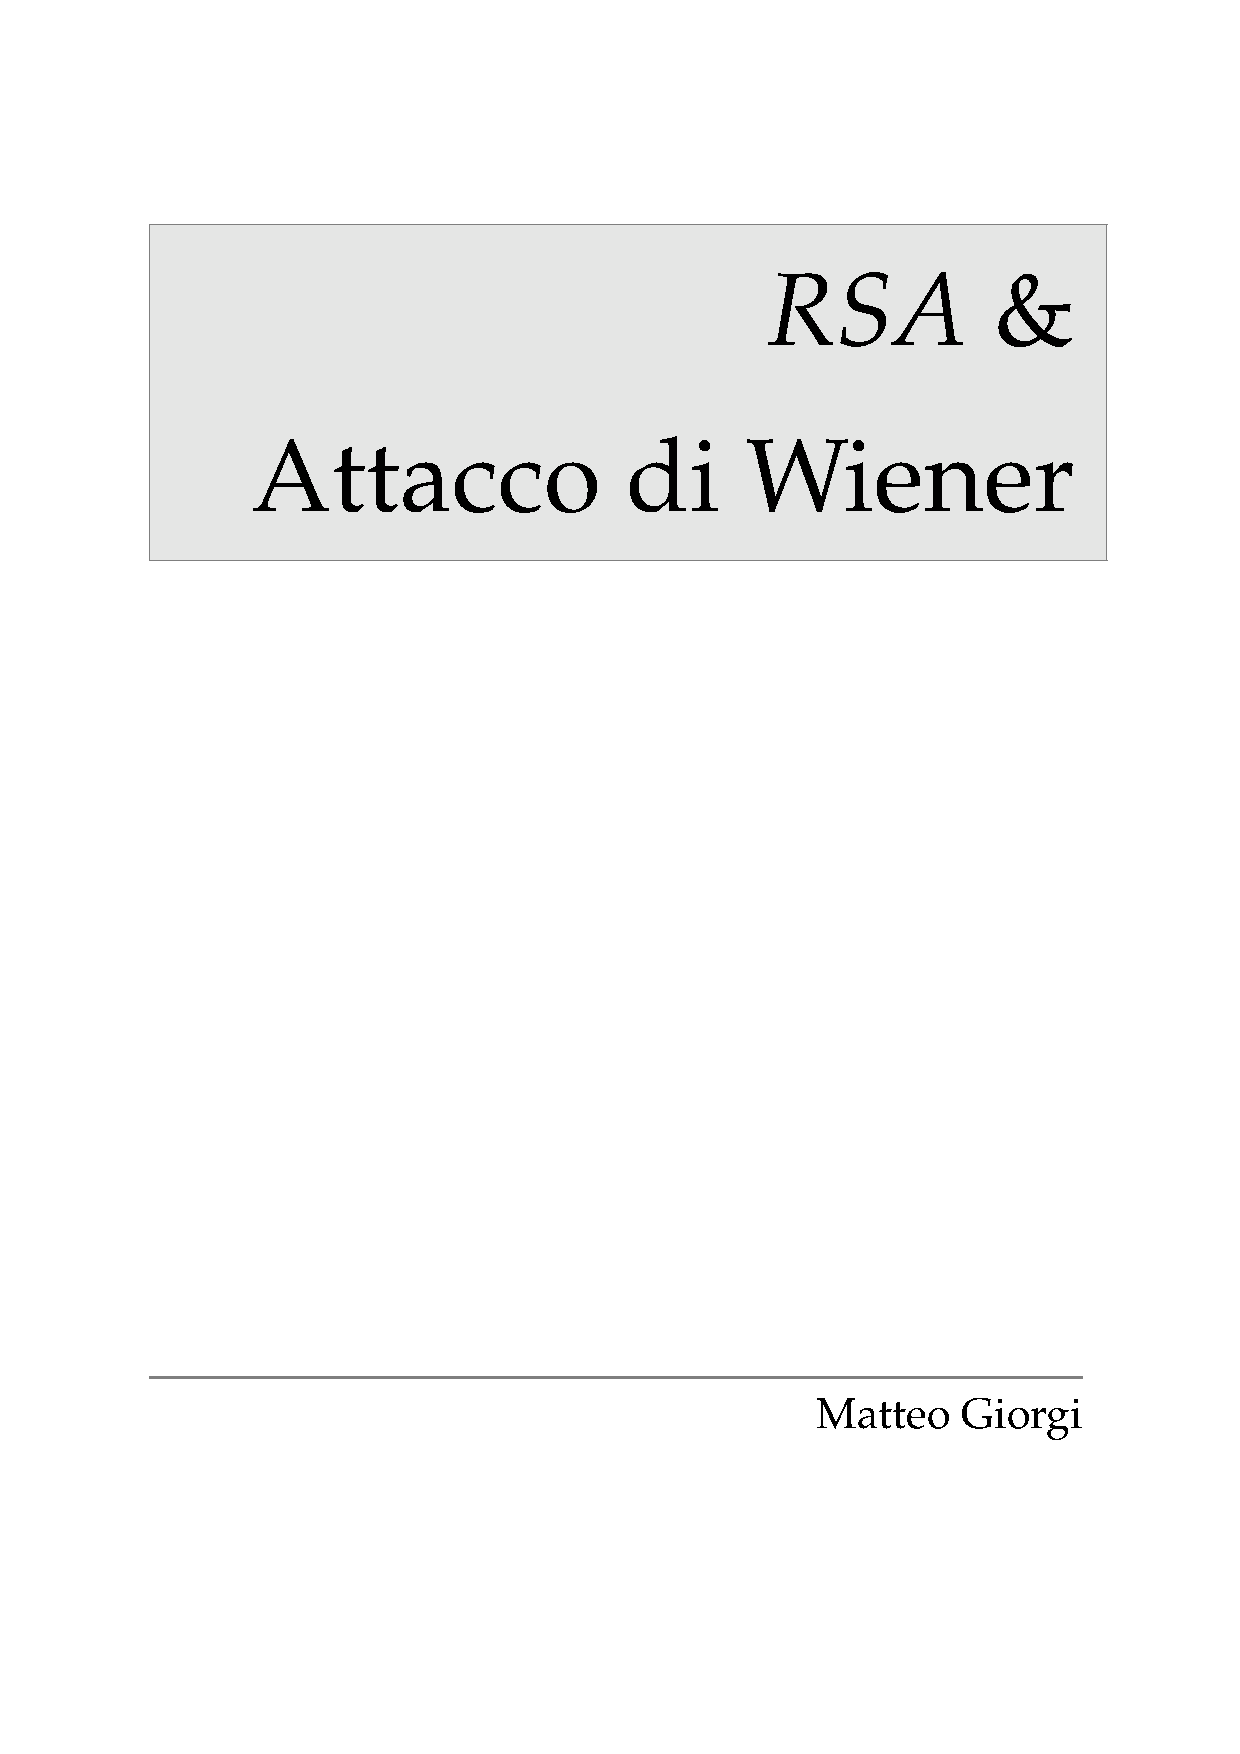
\includepdf{./template/main.pdf}

%%%%%%%%%%%%%%%%%%%%%%%%%%%%%%%%%%%%%%%%%%%%%%%%%%%%%%%%%%%%%%%%%%%%%%%%%%%%%%%%
% \begin{titlepage}
% 	\colorbox{grey}{
% 		\parbox[t]{0.93\textwidth}{
% 			\parbox[t]{0.91\textwidth}{
% 				\raggedleft
% 				\fontsize{50pt}{80pt}\selectfont
% 				\vspace{0.7cm}
				
% 				RSA \&\\
% 				attacco di Wiener\\
				
% 				\vspace{0.7cm}
% 			}
% 		}
% 	}
	
% 	\vfill
	
% 	\parbox[t]{0.93\textwidth}{
% 		\raggedleft
% 		\large
% 		{\huge Matteo Giorgi}\\[4pt]
% 		\hfill\rule{1\linewidth}{1pt}
%   }
% \end{titlepage}
%%%%%%%%%%%%%%%%%%%%%%%%%%%%%%%%%%%%%%%%%%%%%%%%%%%%%%%%%%%%%%%%%%%%%%%%%%%%%%%%

% v.4 copyright page
% \newpage
% \begin{fullwidth}
% ~\vfill
\thispagestyle{empty}

% r.5 contents
% \justify
% \renewcommand\contentsname{}
% \tableofcontents

% \vspace*{123px}
% \begin{fullwidth}
%   \lipsum[2]
%   \begin{itemize}[leftmargin=1in]
%     \item \textsc{Verso il crittosistema RSA}
%     \item \textsc{Attacchi di Wiener}
%   \end{itemize}
%   \lipsum[2]  
% \end{fullwidth}

% r.9 introduction
% \cleardoublepage
% \chapter*{Introduzione}
\vspace*{60px}

\begin{displayquote}
  \textit{Is mathematics ``useful'', directly useful, as other sciences such as
  chemistry and physiology are? This is not an altogether easy or
  uncontroversial question, and I shall ultimately say No\dots}

  \textit{\dots both Gauss and less mathematicians may be justified in rejoicing
  that there is one science at any rate, and that their own, whose very remoteness
  from ordinary human activities should keep it gentle and clean.}

  % \bigskip
  % \rightline{{\rm --- G.H. Hardy, A Mathematician's Apology, 1940}}
  \raggedleft
  --- G.H. Hardy, A Mathematician's Apology, 1940
\end{displayquote}

\vspace*{0.75cm}
\begin{marginfigure}
  \vspace*{-0.3cm}
  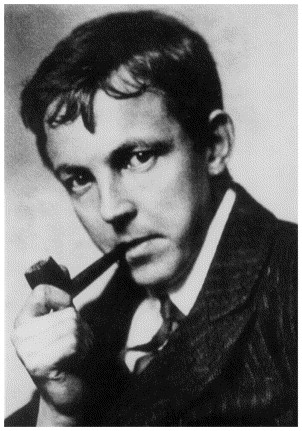
\includegraphics{hardy_pipe.jpg}
  % \caption{Godfrey Harold Hardy (1877 \textendash\xspace 1947)}
  \begin{center}Godfrey Harold Hardy\\ (Cranleigh 1877 -- Cambridge 1947)\end{center}
  \label{fig:marginfig}
\end{marginfigure}

\vspace*{-0.75cm}
\bigskip
\noindent
Oramai a oltre settant'anni dalla pubblicazione della sua famosa Apologia, mi sono
sempre chiesto che cosa direbbe Hardy riguardo l'evoluzione della matematica moderna,
la Teoria dei numeri e le applicazioni pratiche che questa ha indotto nell'ultimo mezzo secolo.
Proprio la sua Teoria dei numeri, descritta da Gauss come la regina delle matematiche per la sua ``suprema inutilità'',
è stata la base per nuovi settori della matematica applicata come la \textit{Teoria computazionale dei numeri}
e la \textit{Crittografia asimmetrica}.

Questo lavoro vuole essere un percorso alla scoperta del crittosistema $RSA$ e
nello specifico delle conseguenze che il Teorema di Wiener ha portato.

\newpage
\vspace*{0.7cm}
\tableofcontents
\vspace*{\fill}
% \begin{center}
%   \color{black!50}
%   \line(1,0){480}
% \end{center}
\begin{fullwidth}
  \color{black!50}
  % \line(1,0){480}\\
  \hfill\rule{1\linewidth}{1pt}
  \footnotesize
  \color{black}
  Nel testo sono usati i nomi che abitualmente si trovano in Letteratura per le comunicazioni cifrate: il mittente \A, il destinatario \B ed il crittoanalista \OS che cerca di carpire il messaggio della conversazione.
  
  % \noindent
  Riguardo la notazione, è necessario fornire chiarimenti su quella usata. Il campo finito $\nicefrac{\mathbb{Z}}{p\mathbb{Z}}$ degli interi modulo un primo $p$, spesso denotato con $\mathbb{F}_p$ o $GF(p)$, è qui indicato con il simbolo $\mathbb{Z}_p$ (in alcuni testi usato invece per gli anelli di interi p-adici), mentre $\mathbb{Z}^*_p$ si riferisce al gruppo delle unità, o gruppo moltiplicativo, di $\nicefrac{\mathbb{Z}}{p\mathbb{Z}}$. Dati $a,b{\in}\mathbb{Z}_p$, la relazione di uguaglianza è qui denotata dalla congruenza modulo $p$: $a{\equiv}b\, (mod\,p)$ oppure $a\,{\equiv}_{\text{\tiny $p$}}b$. In ultimo, $\mathbb{Z}\textsuperscript{+}$ indica il sottoinsieme degli interi positivi.
  % \noindent
  % \color{black!50}
  % \hfill\rule{1\linewidth}{1pt}
\end{fullwidth}
\begin{displayquote}
  \begin{fullwidth}
    \raggedleft\footnotesize
    \textit{All notation should be as simple as the nature of the operation to which is applied.}

    % \bigskip
    % \rightline{{\rm --- C. Babbage}}
    --- C. Babbage
  \end{fullwidth}
\end{displayquote}
% \begin{fullwidth}
%   \footnotesize\raggedleft
%   --- C. Babbage
% \end{fullwidth}



% \includepdf[scale=.7]{escher_stars.pdf}
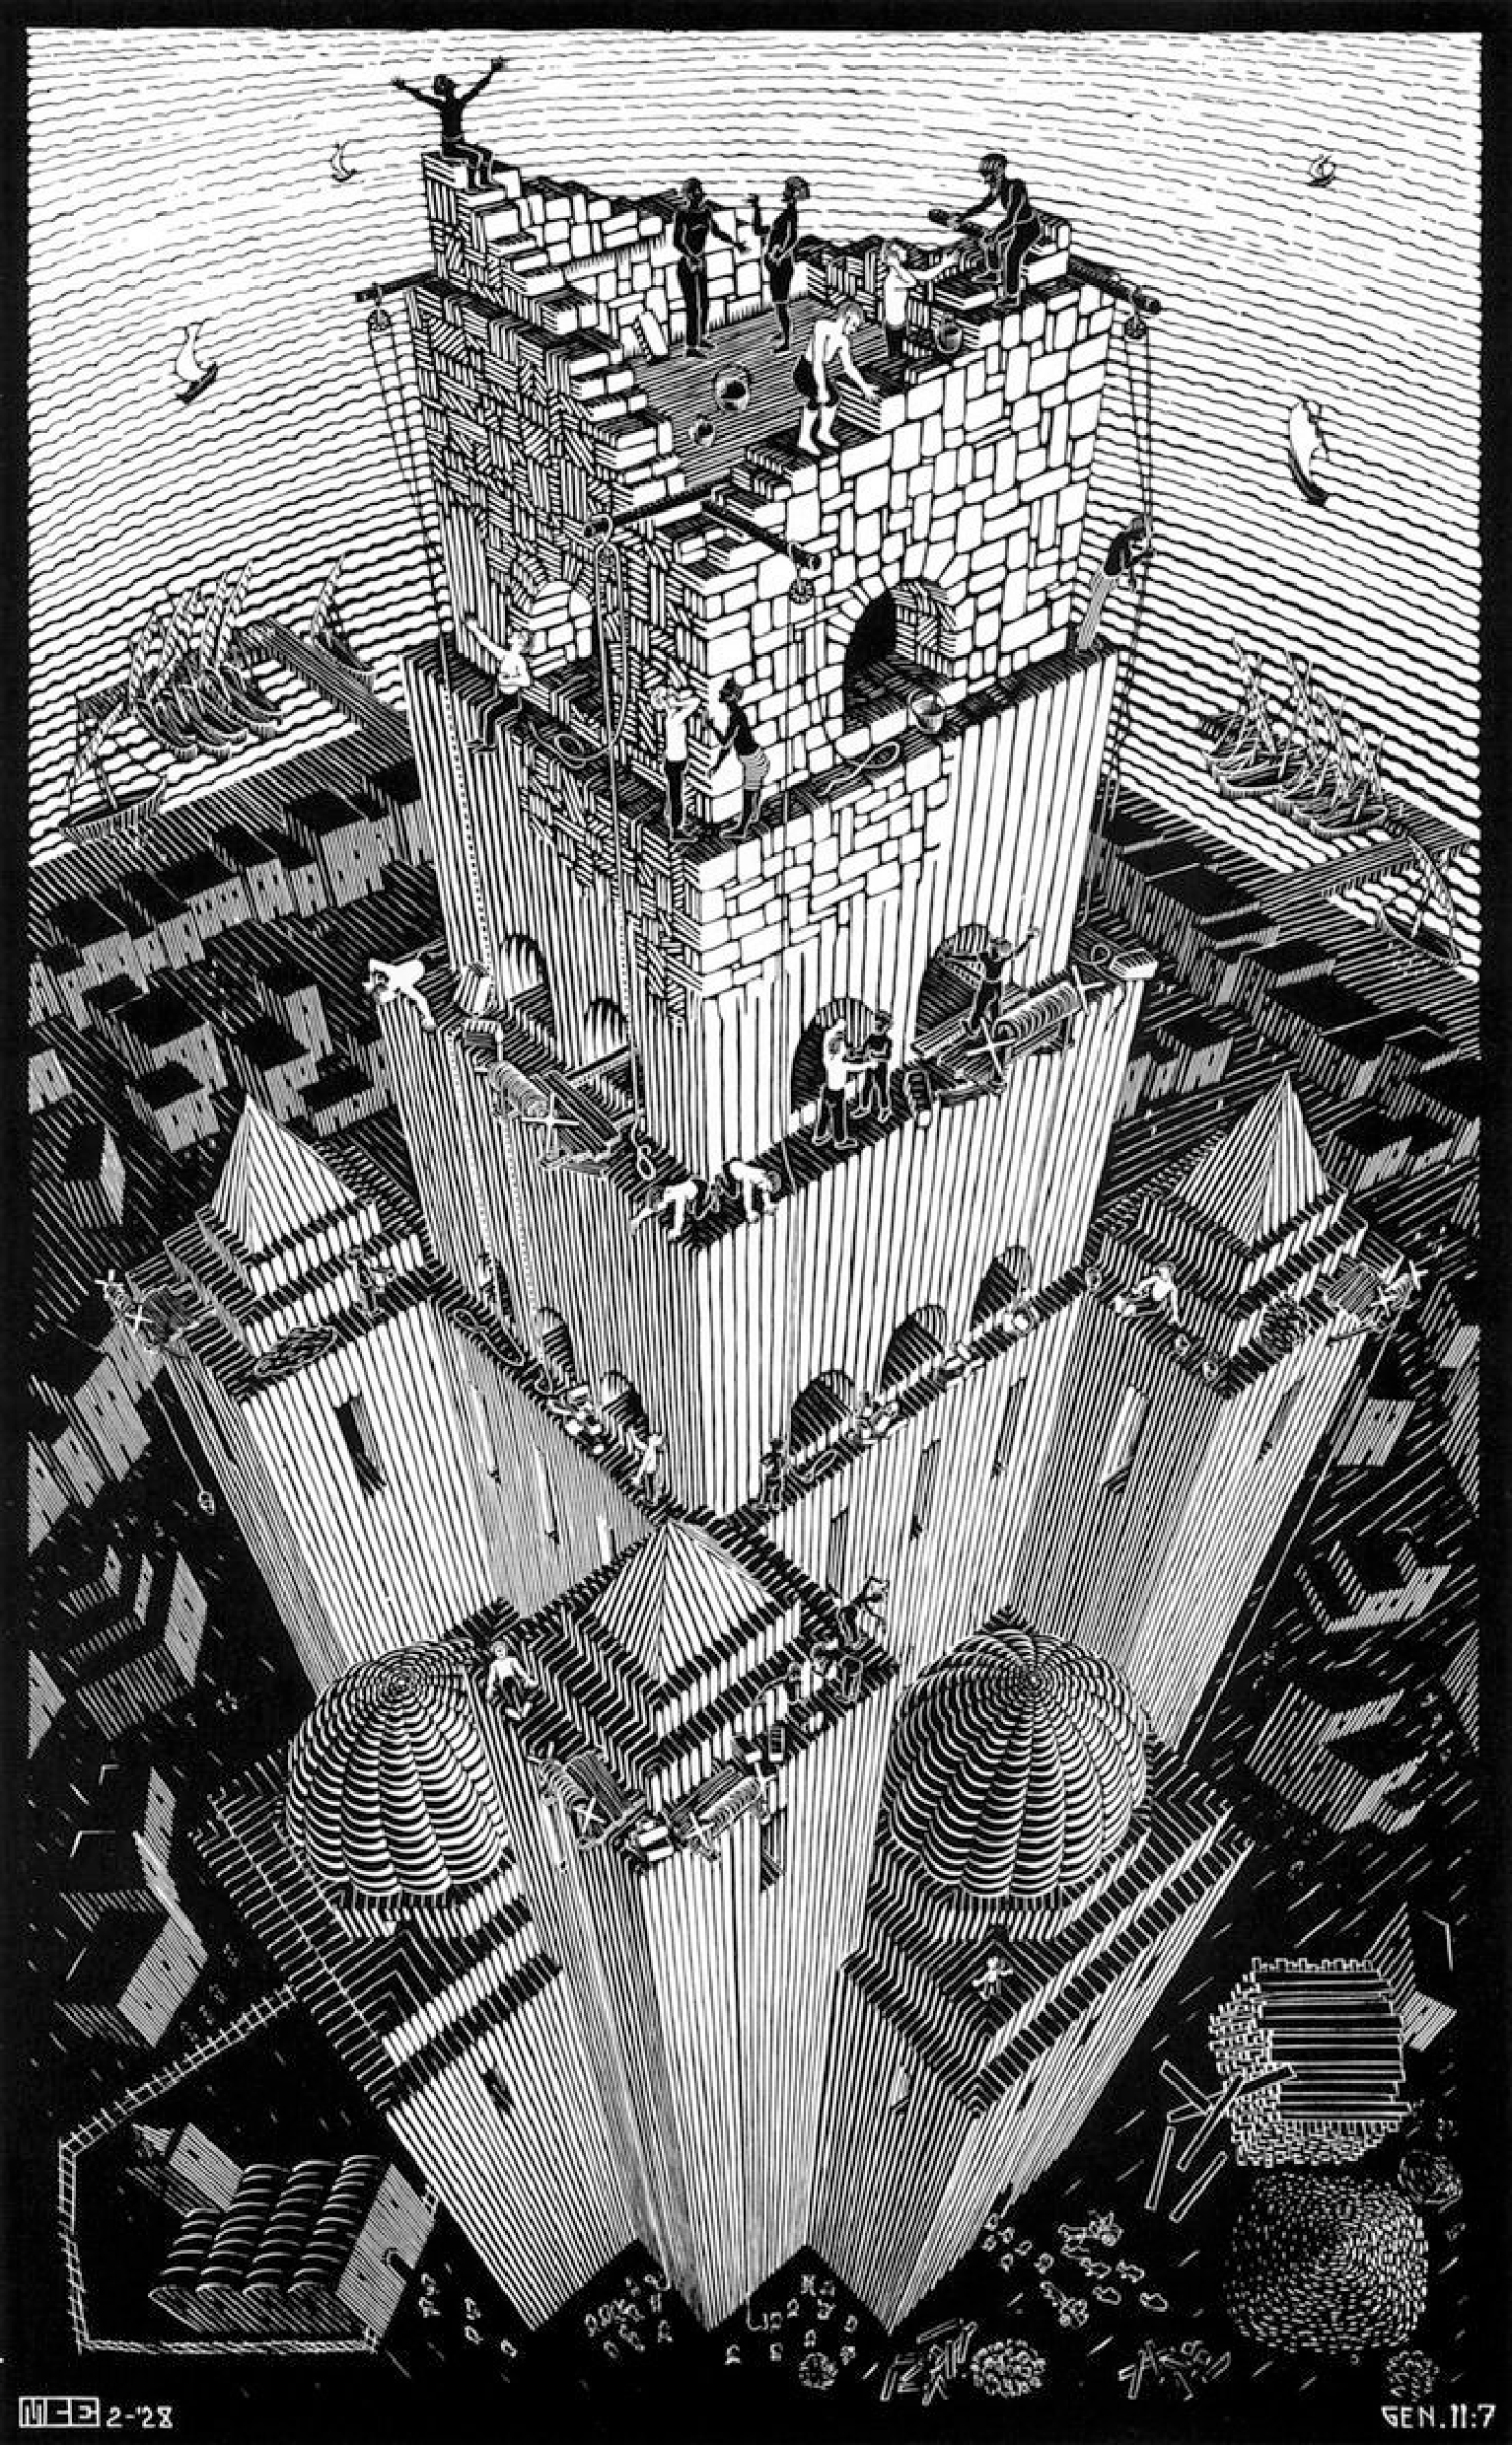
\includepdf[scale=.75]{escher_babel_2.pdf}
% \includepdf[scale=.7]{alice_2.pdf}
%%
% Start the main matter (normal chapters)
\mainmatter

\chapter*{\normalfont\textbf{Verso il crittosistema \boldmath$RSA$}}\label{ch:verso-rsa}
\chaptermark{Verso il crittosistema RSA}
\addcontentsline{toc}{chapter}{Verso il crittosistema \boldmath$RSA$}

Per\marginnote[-24pt]{
  % \begin{mdframed}[linecolor=black, backgroundcolor = verylightgray]
  % \justify
  % \vspace{-0.9cm}
  \newthought{U}no dei più importanti algoritmi simmetrici della crittografia moderna è il \textit{Data encryption Standard} o DES, sviluppato negli anni '70 dalla IBM e adottato nel 1977 come \textit{Federal Information Processing Standard} per gli US. Nella sua forma base il DES non è più considerato sicuro per la chiave di soli 56 bit, vulnerabile ad attacchi brute-force. Rimane comunque in grande uso oggi nella sua forma modificata \textit{Triple-DES}.
  
  % \noindent
  Michael Wiener, nel 1993 alla conferenza \mbox{CRYPTO}, propose un efficiente key-search con tecniche pipeline, stimando un tempo di ricerca medio di 36 ore ed un costo totale di un milione di dollari.

  % \medskip
  Nel 1998 la \textit{Electronic Frontier Foundation}, con un budget di 250,000 dollari, costruì \textit{Deep Crack} capace di una ricerca esaustiva della chiave in 56 ore. Nel 2006 un team di ricercatori delle università di Bochum e Kiel realizzò \mbox{COPACOBANA}, una macchina composta da 120 FPGA, in grado di rompere il DES in 7 giorni con un budget di soli 10,000 dollari. Questo decretò il definitivo pensionamento del DES in favore del nuovo standard \textit{Advanced Encryption Standard} (AES).
  % \end{mdframed}
} comprendere appieno i principi della \textit{crittografia asimmetrica}, è necessario ricapitolare le basi della cifratura simmetrica.

\begin{marginfigure}[0pt]
  \hspace{-2pt}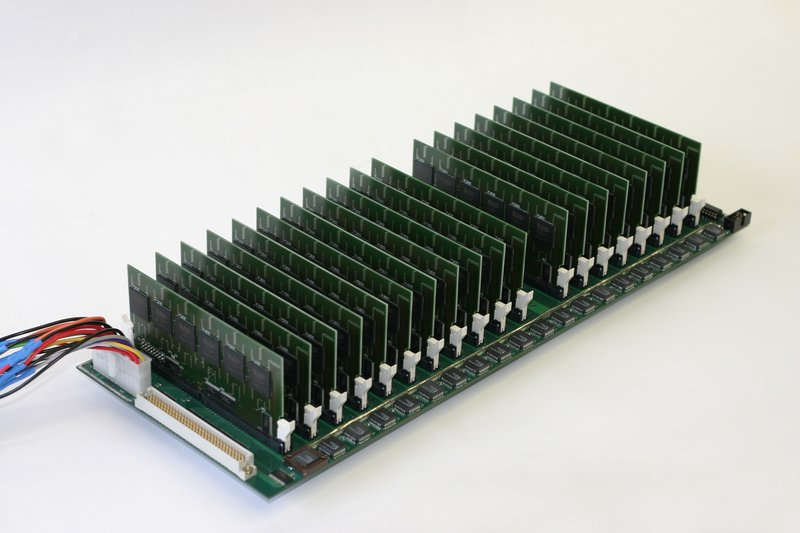
\includegraphics[width=\linewidth]{copacobana.jpg} %5.06cm
  \vspace{-8pt}\caption{versione aggiornata al 2008 di COPACOBANA con 128 Virtex-4 SX35. Il tempo medio è sceso a 6 giorni, quello al caso pessimo a meno di 13.
  % (\url{http://www.copacobana.org/})}
  }
  \label{fig:marginfig}
\end{marginfigure}
\marginnote[-1pt]{\hfill{\color{ForestGreen}$\rightsquigarrow\ $}\url{www.copacobana.org}}

Un sistema simmetrico è tale se un'unica chiave segreta è usata per cifrare/decifrare il testo e le funzioni di cifratura/decifrazione sono simili tra loro.
\A dovrà quindi cifrare il messaggio usando una chiave segreta $k$ e spedirlo su un canale insicuro a \B che decifrerà il crittogramma con la medesima chiave.

I moderni algoritmi simmetrici come AES o Triple-DES sono sicuri e largamente utilizzati, tuttavia presentano dei limiti.

% \begin{description}[nosep, leftmargin=.15in, labelindent=0in]
\begin{description}[nosep, leftmargin=.22in, labelindent=0in]
  \item[\circled{$\star$}] Distribuzione delle chiavi: la chiave deve essere stabilita tra \A e \B usando un canale sicuro.
  \item[\circled{$\star$}] Elevato numero di chiavi: in una rete con $n$ utenti sono necessarie $\mathcal{O}(n^{2})$ coppie di chiavi ed ogni utente deve archiviare in modo sicuro $n{-}1$ chiavi per poter comunicare.
  \item[\circled{$\star$}] Vulnerabilità alle ``truffe'': con un'unica chiave privata, la crittografia simmetrica non fornisce sicurezze sull'identità degli utenti.
\end{description}

\noindent
Questi problemi furono risolti a metà degli anni '70 quando un matematico del MIT Whitfield Diffie ed un ingegnere di Stanford Martin Hellman avanzarono una
% \href{https://www-ee.stanford.edu/~hellman/publications/24.pdf}{nuova idea}
nuova idea rivoluzionaria basata sul presupposto che il crittogramma potesse essere decifrato unilateralmente: \B rilascia pubblicamente una chiave $k_{pub}$ usata da \A per cifrare il messaggio e spedirlo, sicura del fatto che solamente \B potrà decifrarlo grazie ad una seconda chiave privata $k_{priv}$ in suo possesso. Nasce così la \textit{crittografia asimmetrica} \cite{diffie-hellman}.

La base per costruire un tale algoritmo risiede nel cifrare con una funzione \textit{One-Way Trapdoor}: facile da eseguire, ma computazionalmente difficile da invertire a meno di possedere una specifica chiave privata. Questa scelta è sufficiente per proteggersi da \OS che altrimenti potrebbe risalire al messaggio invertendo la funzione di cifratura.

Oggi sono i \textit{protocolli ibridi} come SSL/TLS o IPsec i più utilizzati: un algoritmo asimmetrico per scambiare la chiave segreta $k$ in sicurezza, uno simmetrico per cifrare velocemente il testo da inviare.

\newpage
\section*{\normalfont\textbf{Il crittosistema $\boldsymbol{RSA}$}}\label{sec:crittosistema-rsa}
\addcontentsline{toc}{section}{Il crittosistema $RSA$}
\mnoteskip{-19pt}{
  % \justify
  % \vspace{-.5cm}
  \begin{definizione}[\textsc{$\phi$ di Eulero}]\
    \label{def1}
    
    Dato $n{\in}\mathbb{Z}\SP{+}$, la \textit{funzione di Eulero} $\phi(n)$ è definita come il numero di classi di resto modulo $n$ coprime con $n$:
    \[
      \phi(n)\overset{def}{=}\{ z{\in}\mathbb{Z}\SB{n} \mid MCD(z,n){=}1\}
    \]
  \end{definizione}

  \begin{definizione}[\textsc{$\mu$ di M\"obius}]\

    Dato $n{\in}\mathbb{Z}\textsuperscript{+}$, la funzione di M\"obius $\mu(n)$ è definita come:
    \[
      \hspace{3pt}\mu(n)\overset{def}{=}
      \begin{cases}
        1 &\text{\scriptsize se } n{=}1\\
        0 &\text{\scriptsize se } \exists\ p^2|n,\, p\, \text{\scriptsize primo}\\
        ({-}1)^k &\text{\scriptsize se } n{=}\prod^{k}_{i=1}p_{i}
      \end{cases}
    \]
    % \begin{enumerate}[nosep]
    %   \item $\mu(1){=}1$
    %   \item $\mu(n){=}0$ se $n$ ha un fattore quadrato
    %   \item $\mu(\prod^{k}_{i=1}p_{i}) {=} ({-}1)^k$ se $p_i{\neq}p_j$ ${\forall}i{\neq}j$.
    % \end{enumerate}
  \end{definizione}

  \begin{lem}[$\phi\propto\sum\mu$]
    \label{lemma1}
    Sia $n{\in}\mathbb{Z}\textsuperscript{+}$:
    \begin{equation}
      \phi(n) = \underset{d|n}{\sum}\,n\frac{\mu(d)}{d}
    \end{equation}
  \end{lem}

  \begin{proof}
    Sia $m{\in}\mathbb{Z}\textsuperscript{+}$. Allora:
    \[
      \hspace{4pt}\sum_{d|m}\mu(d){=}
      \begin{cases}
        \hspace{3.5pt} 1 &\text{\scriptsize se }m{=}1\\
        % \begin{array}{c}
          \underset{
            \text{\scalebox{0.95}{$\color{red}\rotatebox[origin=t]{150}{$=$}\overset{k}{\underset{i=1}{\sum}}\text{\scalebox{0.7}{$\dbinom{k}{i}$}}1^{k-i}({-}1)^i$}}
          }{\color{red}\boxed{\color{black}0}} &\text{\scriptsize se }m{>}1
          % \overset{k}{\underset{i=1}{\sum}}\text{\scalebox{0.7}{$\dbinom{k}{i}$}}1^{k-i}({-}1)^i
          % \hspace{-30pt}\scalebox{0.8}{\rotatebox[origin=t]{135}{$=$}$\overset{k}{\underset{i=1}{\sum}}\text{\scalebox{0.7}{$\dbinom{k}{i}$}}1^{k-i}({-}1)^i$}
        % \end{array}
      \end{cases}
    \]
    
    % $m{=}1$ \hspace{-1pt}$\Rightarrow$ $\sum_{d|m}\mu(d){=}1$,\
    
    % $m{>}1$ $\Rightarrow$ $\sum_{d|m}\mu(d) {=} \sum^{k}_{i=1}$\scalebox{0.7}{$\dbinom{k}{i}$}$1^{k-i}({-}1)^i{=}0$\
    
    % e posso affermare che ${\sum_{d|m}}\mu(d) {=} \lfloor \nicefrac{1}{m}\rfloor$.
    % Quindi, per la Definizione \ref{def1} data sopra:\
    
    % $\phi(n) {=} \sum^{n}_{k=1}\lfloor \nicefrac{1}{(n,k)} \rfloor {=} \sum_{d|(n,k)}\mu(d)$.\
    
    % Adesso, fissato un $d$, divisore di $n$, devo sommare tutti i $k{\in}[1,n]$ multipli di $d$; quindi, se $k{=}qd$, posso scrivere:\
    
    % $\phi(n) {=} \sum_{d|n}\sum^{\nicefrac{n}{d}}_{q=1}\mu(d) {=} \sum_{d|n}\mu(d)\nicefrac{n}{d}$.
    e posso affermare che ${\sum_{d|m}}\mu(d) {=} \lfloor \nicefrac{1}{m}\rfloor$.
    Ora, usando la Definizione \ref{def1} e fissato un $d|n$, posso sommare tutti i $k{=}qd{\in}[1,n]$:
    \[
      \begin{array}{c}
        \phi(n) = \overset{n}{\underset{k=1}{\sum}}\Bigl\lfloor\frac{1}{(n,k)}\Bigr\rfloor = \underset{ \begin{subarray}{c}
                                                                                                              d|n\\
                                                                                                              d|k
                                                                                                            \end{subarray}}{\sum}\mu(d) =\\
        \hspace{20pt}= \underset{d|n}{\sum}\ \overset{\nicefrac{n}{d}}{\underset{q=1}{\sum}}\mu(d) = \underset{d|n}{\sum}n\frac{\mu(d)}{d}\hspace{20pt}\hfill\qedhere
      \end{array}
    \]
  \end{proof}

  \begin{lem}[\textsc{Calcolo} $\phi$]
    \label{lemma2}
    Sia $n{\in}\mathbb{Z}\textsuperscript{+}$:
    \begin{equation}
      \phi(n)=n\, {\underset{p|n}{\prod}}\Bigl(1{-}\frac{1}{p}\Bigr)
    \end{equation}
  \end{lem}

  \begin{proof}
    Per $n{=}1$ la produttoria è vuota perchè non esistono primi divisori di $1$, quindi $\phi(1){=}1$.
    Supponendo invece $n{>}1$, si può esprimere $n{=}{\prod^{k}_{i=1}}p^{\alpha_i}_{i}$
    % ($\{p_{1}, p_{2},\dots, p_k\}$ primi distinti)
    % (prodotto di potenze di primi distinti),
    e, per il \textit{Principio di Inclusione-Esclusione}, la produttoria può essere riscritta come:
    \[
      \begin{array}{c}
        \underset{p|n}{\prod}\bigl(1{-}\frac{1}{p}\bigr) = \overset{k}{\underset{i=1}{\prod}}\bigl(1{-}\frac{1}{p_i}\bigr) =\\
        = 1 {-} {\sum}\frac{1}{p_i} {+} {\sum}\frac{1}{p_i p_j} {+} \dots {+} \frac{({-}1)^k}{{\prod^{k}_{i=1}}p_{i}}
      \end{array}
    \]
    dove ciascun termine è della forma $\nicefrac{\pm1}{d}$. Il denominatore $d$ è un divisore di $n$, prodotto di primi distinti; il numeratore $\pm1$ è esattamente la \textit{Funzione di M\"obius} $\mu(d)$. Quindi la produttoria risulta:
    \[
      \underset{p|n}{\prod}\Bigl(1{-}\frac{1}{p}\Bigr) = \underset{d|n}{\sum}\frac{\mu(d)}{d}
    \]
    che, per il lemma \ref{lemma1}, dimostra la tesi.
  \end{proof}
}

% \vspace{-0.7cm}
% \section*{\normalfont\textbf{Il crittosistema $\boldsymbol{RSA}$}}\label{sec:crittosistema-rsa}
% \addcontentsline{toc}{section}{Il crittosistema $RSA$}

La scelta per una funzione \textit{One-Way Trapdoor} deve ricadere su un'idea concettualmente semplice, facile da implementare ma con una forte prova empirica che la decifrazione non sia possibile a meno di conoscere la chiave segreta. La risposta arriva dalla teoria dei numeri: la fattorizzazione di un intero.

Nel 1977 tre informatici del MIT Ronald Rivest, Adi Shamir e Leonard Edleman esposero il \textit{MIT public-key criptosystem}, successivamente $RSA$, incentrato proprio sulla fattorizzazione di interi ed il Teorema di Eulero-Fermat \cite{rivest-shamir-edleman}.

\begin{thm}[\textsc{Eulero-Fermat}]
  Siano $a$, $n$ interi coprimi. Allora:
  \begin{equation}
    a^{\phi(n)}\equiv 1\quad (mod\ n)
  \end{equation}
\end{thm}

\begin{proof}
  Preso $k{\in}\mathbb{Z}$ coprimo con $n$ e $\{a_{1}, a_{2},\dots,a_{\phi(n)}\}$ insieme delle classi di resto modulo $n$ coprime con $n$, $\{ka_{1}, ka_{2},\dots,ka_{\phi(n)}\}$ è il medesimo insieme perchè:
  \begin{description}[nosep, leftmargin=.22in, labelindent=0in]
    \item[\circled{$1$}] scelte due classi distinte $a_i$, $a_j$ con $i,j{\in}[1,\phi(n)]$ e $i{\neq}j$, posso affermare che $a_i{\not\equiv}_{\text{\tiny $n$}}a_j \Rightarrow ka_i{\not\equiv}_{\text{\tiny $n$}}ka_j$;
    \item[\circled{$2$}] fissato $a{\in}\{a_{1}, a_{2},\dots,a_{\phi(n)}\}$, la congruenza $kx{\equiv}_{\text{\tiny $n$}}a$ ha soluzione $x_{0}{\in}$ $\{a_{1}, a_{2},\dots,a_{\phi(n)}\}$, quindi $x_{0}{\equiv}_{\text{\tiny $n$}}a_i \Rightarrow kx_{0}{\equiv}_{\text{\tiny $n$}}ka_i{\equiv}_{\text{\tiny $n$}}a$.
  \end{description} 
  Pertanto adesso posso scrivere
  \[
    \begin{split}
      \overset{\phi(n)}{\underset{i=1}{\prod}}ax_{i} &\equiv \overset{\phi(n)}{\underset{i=1}{\prod}}x_{i}\quad (mod\ n)\\
      a^{\phi(n)}\, \overset{\phi(n)}{\underset{i=1}{\prod}}x_{i} &\equiv \overset{\phi(n)}{\underset{i=1}{\prod}}x_{i}\quad (mod\ n)
    \end{split}
  \]
  e concludere che $a^{\phi(n)}{\equiv}_{\text{\tiny $n$}} 1$.
\end{proof}
% Analogamente a tutti i crittosistemi a chiave pubblica, è possibile pensare all'RSA, come composto di tre algoritmi calcolabili efficientemente: uno per generare la chiave, che definisce lo \textit{spazio delle chiavi} ed altri due per cifrare e decifrare, che definiscono rispettivamente lo \textit{spazio dei messaggi} e lo \textit{spazio dei crittogrammi}.

% \newthought{Funzionamento RSA.}
\addcontentsline{toc}{subsection}{Funzionamento $RSA$}
% \cftaddtitleline{toc}{subsection}{Funzionamento $RSA$}{}
\paragraph{\normalfont\textbf{\underline{Funzionamento $\boldsymbol{RSA}$.}}} Analogamente agli altri sistemi asimmetrici, l'$RSA$ può essere pensato come composto da tre algoritmi efficientemente calcolabili: un generatore della chiave che definisce lo spazio delle \textit{chiavi} ($\mathcal{K}$), un algoritmo di cifratura e uno di decifrazione che definiscono lo spazio dei \textit{messaggi} ($\mathcal{M}$) e dei \textit{crittogrammi} ($\mathcal{C}$).

\B sceglie dunque due primi molto grandi $p$ e $q$ che tiene segreti e calcola il modulo dell'$RSA$ $N{=}pq$. Sceglie poi un esponente pubblico $e{\in}\mathbb{Z}^{*}_{\phi(N)}$ (unità di $\mathbb{Z}_{\phi(N)}$) e calcola l'esponente privato $d$ tale che $ed\,{\equiv}_{\text{\tiny $\phi(N)$}}1$. Quindi, per ogni possibile chiave $k{=}(N,p,q,e,d){\in}\mathcal{K}$, le funzioni di cifratura e decifrazione sono definite come:

\begin{minipage}[b]{0.45\linewidth}
  \center
  \[
    \begin{split}
      Enc_k:\overset{\overset{\mathbb{Z}_\text{\tiny $N$}}{\shortparallel}}{\mathcal{M}} &\rightarrow \overset{\overset{\mathbb{Z}_\text{\tiny $N$}}{\shortparallel}}{\mathcal{C}}\\
      % enc_k:\cancelto{\mathbb{Z}\textsubscript{n}}{\mathcal{M}}\rightarrow\cancelto{\mathbb{Z}\textsubscript{n}}{\mathcal{C}}
      m &\rightarrow m^e
    \end{split}
  \]
\end{minipage}
\begin{minipage}[b]{0.45\linewidth}
  \center
  \[
    \begin{split}
      Dec_k:\overset{\overset{\mathbb{Z}_\text{\tiny $N$}}{\shortparallel}}{\mathcal{C}} &\rightarrow \overset{\overset{\mathbb{Z}_\text{\tiny $N$}}{\shortparallel}}{\mathcal{M}}\\
      % dec_k:\cancelto{\mathbb{Z}\textsubscript{n}}{\mathcal{C}}\rightarrow\cancelto{\mathbb{Z}\textsubscript{n}}{\mathcal{M}}
      c &\rightarrow c^d
    \end{split}
  \]
\end{minipage}

% and check appropriate spacing for longer ``above" and ``below" text:
% \[
%   A = \VerticalRelations{0}{C}{\veq}{D\neq B}{\vneq} \neq B
% \]

% \noindent
% mentre le chiavi pubblica e privata risultano:

% \medskip
% \begin{minipage}[b]{0.45\linewidth}
%   \center
%   $k_{pub}=(e,n)$
% \end{minipage}
% \begin{minipage}[b]{0.45\linewidth}
%   \center
%   $k_{priv}=(d,p,q)$
% \end{minipage}

\newpage
\noindent
mentre\wmnote{
  % \vspace{-.5cm}
  \begin{thm}[\textsc{Cinese dei resti}]\

    Sia $a,b,m,n{\in}\mathbb{Z}$ con $MCD(m,n){=}1$. Allora ${\exists}!\ x{\in}\mathbb{Z}_{mn}$ tale che:
    \begin{equation}
      \label{tcr}
      \begin{cases}
        x \equiv a\quad (mod\ m)\\
        x \equiv b\quad (mod\ n)
      \end{cases}
    \end{equation}
    % inoltre $x$ è unico modulo $m{\cdot}n$.
  \end{thm}
  \begin{proof}
    Se $\widetilde{t}{\in}\mathbb{Z}$ risolve $a{+}tm{\equiv}_{\text{\tiny $n$}}b$ allora $x{=}a{+}tm$ è soluzione di (\ref{tcr}).\
    % Se $\bar{t}$ fosse soluzione di $x{=}a{+}tm{\equiv}b\ (n)$ allora $x$ risolverebbe (\ref{tcr}). Mostriamo che $\bar{t}$ esiste unico.
    % \begin{description}[nosep, leftmargin=0in, labelindent=0in]
    %   \item[\normalfont{Esistenza:}] la precedente congruenza ha soluzione perchè $(m,n){=}1$ per ipotesi.
    %   \item[\normalfont{Unicità:}] supponiamo $x,y{\in}\mathbb{Z}$ soluzioni del sistema, allora $m,n|b{-}a$. Segue che $mn|b{-}a$, ovvero $x{\equiv}y\ (mn)$.
    % \end{description}
    
    % Esistenza: $(m,n){=}1$ per ipotesi, segue che $a{+}tm{\equiv}b\ (n)$ ha soluzione.\
    Esistenza: ${\exists}\ \widetilde{t}{\in}\mathbb{Z}$ soluzione di $a{+}tm{\equiv}_{\text{\tiny $n$}}b$ perchè $MCD(m,n){=}1$ per ipotesi.\
    
    Unicità: se il sistema ammette due soluzioni $x,y$ allora $m,n|b{-}a$. Segue che $mn|b{-}a$, ovvero $x\,{\equiv}_{\text{\tiny $mn$}}y$.
    % ${\exists}!\ \bar{t}$ soluzione di $a{+}tm{\equiv}b\ (n)$: l'esistenza di $\bar{t}$ è assicurata dall'ipotesi $MCD(a,n){=}1$; per l'unicità invece supponiamo esistano $x,y{\in}\mathbb{Z}$ soluzioni di (\ref{tcr}), allora $z{=}x{-}y$ soddisferebbe 
  \end{proof}
  \begin{definizione}[\textsc{$\lambda$ di Carmichael}]\
    \label{def3}
  
    Dato $n{\in}\mathbb{Z}\textsuperscript{+}$, la \textit{funzione di Carmichael} $\lambda(n)$ è definita in termini di $\phi(n)$:
    \[
      % \begin{array}{c}
        \hspace{3pt}\lambda(n)\overset{def}{=}
        \begin{cases}
          % \phi(2^\alpha)\quad n{=}2^\alpha,\ \alpha{=}0,1,2\\
          \frac{1}{2}\phi(2^\alpha) &\text{\scriptsize se } n{=}2^\alpha,\ \alpha{>}2\\
          \phi(p^{\alpha}_{1}) &\text{\scriptsize se } n{=}p^{\alpha}_{1}\\
          \underset{i=1{\dots}k}{mcm\bigl(\lambda(p^{\alpha_i}_i)\bigr)} &\text{\scriptsize se } n{=}{\prod^{k}_{i=1}}p^{\alpha_i}_{i}
        \end{cases}
        % \lambda(p^\alpha)=\phi(p^\alpha)\quad se\ p\ primo\\
        % \lambda(2^{\alpha}{\cdot}p^{\alpha\textsubscript{1}}_{\textit{1}}{\cdot}...{\cdot}p^{\alpha_n}_n)=mcm(\lambda(2^\alpha),\lambda(2^\alpha),...,\lambda(2^\alpha))
        % \lambda(n)=mcm\bigl(\lambda(p^{\alpha_i}_i)\bigr)
      % \end{array}
    \]
    % {\scriptstyle *con\ p\ e\ p_i\ interi\ primi.}
    con $\alpha{\in}\mathbb{Z}\textsuperscript{+}$, $p_{i\in{\{1{\dots}k\}}}{\in}\mathbb{Z}\textsuperscript{+}$ primi.
  \end{definizione}

  \begin{lem}
    Siano $a$, $n$ interi coprimi.\
    Allora:
    \begin{equation}
      a^{\lambda(n)}\equiv 1\quad (mod\ n)
    \end{equation}
  \end{lem}

  \begin{proof}
    In accordo con la Definizione \ref{def3}:
    \[
      \begin{array}{c}
        \hspace{-20pt}\text{se}\ n{=}2^\alpha \Rightarrow \phi(n){=}2\lambda(n)\\
        \hspace{25pt}\Rightarrow a^{\lambda(n)}{\equiv}1\ (mod\ n)
      \end{array}
    \]
    \[
      \begin{array}{c}
        \hspace{-24pt}\text{se}\ n{=}p^{\alpha}_{1} \Rightarrow \phi(n){=}\lambda(n)\\
        \hspace{26pt}\Rightarrow a^{\lambda(n)}{\equiv}1\ (mod\ n)
      \end{array}
    \]
    \[
      % \begin{array}{c}
      \hspace{3pt}\text{se}\ n{=}\overset{k}{\underset{i=1}{\prod}}p^{\alpha_i}_{i} \Rightarrow \underset{\text{per}\ j{\in}\{1{\dots}k\}}{\lambda(n){=}x_j\lambda\bigl(p^{\alpha_j}_j\bigr)}
    \]
    \[
      \hspace{23pt}\Rightarrow
      \begin{cases}
        \bigl(a^{\lambda(p^{\alpha_{\text{1}}}_{1})}\bigr)^{x_{\text{1}}}{\equiv}1\ \bigl(mod\ p^{\alpha_{\text{1}}}_{1}\bigr)\\
        \bigl(a^{\lambda(p^{\alpha_{\text{2}}}_{2})}\bigr)^{x_{\text{2}}}{\equiv}1\ \bigl(mod\ p^{\alpha_{\text{2}}}_{2}\bigr)\\
        \hspace{6}\vdots\\
        \bigl(a^{\lambda(p^{\alpha_{\text{\scalebox{0.8}{$k$}}}}_{k})}\bigr)^{x_{\text{\scalebox{0.8}{$k$}}}}{\equiv}1\ \bigl(mod\ p^{\alpha_{\text{\scalebox{0.8}{$k$}}}}_{k}\bigr)
      \end{cases}
      % \end{array}
    \]
    \begin{minipage}[c]{0.25\linewidth}
      \center\tiny\color{red}
      % \hspace{100pt}$\overwritecinese
        % {\color{red} \boxed{\color{black} \Rightarrow}}
        % {\tiny\textit{Th. cinese} \tiny\textit{dei resti}}$
        \hspace{-17pt}{\textit{Th. Cinese}}\\
        \hspace{-17pt}{\textit{dei Resti}}
    \end{minipage}
    \begin{minipage}[c]{0.45\linewidth}
      \center
      \hspace{-45pt}${\color{red}\boxed{\color{black}\Rightarrow}}\ a^{\lambda(n)}{\equiv}_{\text{\tiny $n$}}1$.
    \end{minipage}\qedhere

    % \[
      % \begin{array}{c}
        % \hspace{-39}{\color{red}\boxed{\color{black}\Rightarrow}}\ a^{\lambda(n)}{\equiv}1\ (n)\\

        % \overwritecinese
        %   {\color{red} \boxed{\color{black} \Rightarrow}}
        %   {\tiny\textit{Th. cinese} \tiny\textit{dei resti}}
        %   {a^{\lambda(n)}{\equiv}1\ (n)}
        
        % \hspace{-39}{\color{red}\overset{\text{\tiny Th. cinese}}{\Rightarrow}}\ a^{\lambda(n)}{\equiv}1\ (n)
        % \hspace{-100pt} {\color{red}\rotatebox[origin=c]{225}{$\rightsquigarrow$}}\\
        % \hspace{-100pt}\text{\tiny\color{red}\textit{Th. cinese dei resti}}
        % \hspace{-100pt}\text{\tiny\color{red}\textit{dei resti}}
      % \end{array}
    % \]
    % e quindi per il \textit{Teorema cinese dei resti} $a^{\lambda(n)}{\equiv}1\ (n)$.
  \end{proof}
}le chiavi pubblica e privata risultano:

\medskip
\begin{minipage}[b]{0.45\linewidth}
  \center
  $k_{pub}=(e,N)$
\end{minipage}
\begin{minipage}[b]{0.45\linewidth}
  \center
  $k_{priv}=(d,p,q)$
\end{minipage}

\medskip
% \vspace{.5cm}
\noindent
A questo punto è chiaro come la correttezza della funzione di decifrazione $Dec_k$ risieda nel Teorema di Eulero-Fermat, sia nel caso in cui $MCD(m,N){=}1$, che altrimenti:
% \[
%   m = c^d = (m^e)^d = \boxed{m^{1+\phi(n)} \equiv m\,(n)}
%   _{se\, \mathcal{MCD}(m,n){=}1\, \Rightarrow\, m^{\phi(n)}{\equiv}1\,(n)\, \Rightarrow\, m^{1+\phi(n)}\equiv m\, (n)}
%   c^d \equiv (m^e)^d \equiv m^{1+\phi(n)} \equiv m\,(n)  
% \]
\[
  \hspace{-50pt}{\begin{array}{c}
      m \equiv c^d \equiv \bigl(m^e\bigr)^d = \boxed{m^{1+k\phi(N)} \equiv m\quad (mod\ N)}\\
      \hspace{85pt} \downarrow\\
      % a\mbox{th position}
      \hspace{85pt} {
        % \scriptstyle se\,
        \text{\scriptsize se}\,
        \scriptstyle{MCD(m,N){=}1\ \Rightarrow\ m^{\phi(N)}{\equiv}_{\text{\tiny $N$}}1\ \Rightarrow\ m^{1+k\phi(N)}{\equiv}_{\text{\tiny $N$}} m}
      }\\
      \hspace{85pt} {
        % \scriptstyle altrimenti\
        \text{\scriptsize altrimenti}\
        {\scriptsize\begin{cases}
          m^{1+r\phi(N)}{\equiv}_{\text{\tiny $p$}}m\\
          m^{1+s\phi(N)}{\equiv}_{\text{\tiny $q$}}m
        \end{cases}}
        \hspace{-8pt}{
          \overwrite{\color{red}\boxed{\color{black}\Rightarrow}}{\tiny\textit{Th. Cinese dei Resti}}\ \hspace{-6pt}{\scriptstyle m^{1+k\phi(N)}{\equiv}_{\text{\tiny $N$}} m}
        }
      }
  \end{array}}
\]
Certamente, messaggi coprimi con il modulo dovrebbero essere evitati perchè il relativo crittogramma $c$ rivelerebbe la fattorizzazione del modulo stesso: in particolare, eseguire $MCD(c,N)$ individuerebbe un multiplo di uno dei primi $p$ e $q$.

Definire gli esponenti pubblico e privato come inversi modulo $\phi(N)$ fornisce una condizione sufficiente per recuperare il messaggio da qualsiasi crittogramma, mentre la condizione necessaria è che siano inversi modulo $\lambda(N)$, \textit{Funzione di Carmichael}. Quindi, dato il modulo $N$, $\lambda(N){=}mcm(p{-}1,q{-}1)$ e:
% quindi $\phi(n)$ è multiplo di $\lambda(n)$:
\[
  \begin{split}
    \phi(N) &= (p{-}1)(q{-}1)\\
    &=MCD(p{-}1,q{-}1)\ mcm(p{-}1,q{-}1)\\
    &=MCD(p{-}1,q{-}1)\ \lambda(N)
  \end{split}
\]
% \[
%   \phi(n)=(p{-}1)(q{-}1)
% \]
% \[
%   \hspace{123pt}=MCD(p{-}1,q{-}1)\cdot mcm(p{-}1,q{-}1)
% \]
% \[
%   \hspace{74pt}=MCD(p{-}1,q{-}1)\cdot \lambda(n)
% \]
ovvero $\lambda(N)|\phi(N)$, il che ci permette di usare $\phi(N)$ nell'algoritmo generatore della chiave. Nel corrente standard \hyperlink{pkcs1}{\textit{PKCS $\#1$}} i due esponenti pubblico e privato sono definiti come inversi modulo $\lambda(N)$.

% \subsection{Sicurezza e Efficienza}\label{sec:sicurezza-efficienza}\index{headings}
% \newthought{Sicurezza e efficienza.} \lipsum[1]

% \paragraph{\normalfont\textbf{Sicurezza \& Efficienza.}}
% \begin{fullwidth}
%   \lipsum[3]
% \end{fullwidth}

\section*{\normalfont\textbf{Attacchi elementari}}\label{sec:elementary-attack}
\addcontentsline{toc}{section}{Attacchi elementari}
Gli attacchi al crittosistema $RSA$ sono generalmente classificabili in diverse famiglie. Gli attacchi \textit{algoritmici diretti} sono quelli di più immediata intuizione e si suddividono in attacchi sulla fattorizzazione intera, logaritmo discreto e attacchi quantistici. Da notare invece che gli attacchi migliori cercano di sfruttare le debolezze matematiche dell'algoritmo o un improprio uso del sistema (un esponente piccolo o il medesimo modulo su più comunicazioni): questi sono gli attacchi \textit{algoritmici indiretti} e saranno l'oggetto del resto di questo lavoro.
A titolo informativo è giusto citare anche gli attacchi \textit{side-channel}: essi sfruttano specifici problemi di implementazione dell'hardware, come il consumo energetico o il tempo di cifratura/decifrazione del dispositivo, per recuperare la chiave segreta.

Di seguito alcuni attacchi algoritmici elementari indiretti.

\vspace{-2cm}%-1.7
\begin{marginfigure}
  % \vspace{-0.6cm}
  \includegraphics[width=5.6cm]{security.png}
  % \begin{changemargin}{0.3cm}{0cm} 
  %   \textit{Quanto deve essere grande il modulo per essere considerato sicuro?}
  % \end{changemargin}
  \label{fig:marginfig}
\end{marginfigure}
\marginnote[-14pt]{
  \hspace{4pt}\begin{minipage}[b]{0.45\textwidth}
    \captionof{figure}{Crypto-Brainstorming.}
  \end{minipage}
}

\vspace{1.7cm}
\addcontentsline{toc}{subsection}{Stima $\phi(N)$}
\paragraph{\normalfont\textbf{\underline{Stima $\boldsymbol{\phi(N)}$.}}} Se \OS potesse conoscere il valore di $\phi(N)$,
\marginnote{
  \vspace{-0.85cm}
  \textbf{\textit{\newthought{\textit{Q}}uanti bits deve avere il modulo per essere considerato sicuro?}} \par
  Nel 1999 gli RSA-Laboratories impiegarono sette mesi per fattorizzare un intero di $515${\normalfont\texttt{b}} ($155$ cifre decimali) nel prodotto di due primi da $77${\normalfont\texttt{b}}: non male! \par
  Nel 2004, per una chiave che rimanesse sicura fino al 2010, raccomandavano l'utilizzo di moduli da $1024${\normalfont\texttt{b}} (fattorizzabili in primi da $154${\normalfont\texttt{b}}), mentre per una sicurezza più a lungo termine (2030) sono tuttora necessari almeno $2048${\normalfont\texttt{b}}.
  
  \hfill {\color{ForestGreen}$\rightsquigarrow\ $}\url{www.rsa.com}
}potrebbe facilmente recuperare $m$ in tempo polinomiale: $\phi(N)\overset{\mathcal{P}}{\Rightarrow}\{m\}$.

\noindent
Sarà dunque necessario mostrare che il calcolo di $\phi(N)$ e l'\textit{Integer Factorization Problem} ($IFP$), ovvero la fattorizzazione del modulo, sono asintoticamente equivalenti.

\begin{thm}
  \label{ifp}
  \begin{equation}
    \label{eq-ifp}
    \phi(N)\overset{\mathcal{P}}{\Longleftrightarrow} IFP(N)
  \end{equation}
\end{thm}

\begin{proof}
  Essendo $\phi(N){=}(p{-}1)(q{-}1)$ noto, si ottiene che
  \begin{equation}
    \label{stima}
    \begin{array}{c}
      % \phi(n)=(p-1)(q-1)\\
      % pq-p-q+1-\phi(n)=0\\
      p^{2}-\underbrace{\bigl(N{-}\phi(N){+}1\bigr)}_{p+q=A}p+\tiny\underbrace{\scalebox{2}{$N$}}_{p\cdot q}=0\\
      \text{\scriptsize quindi}\ \
      % \rightsquigarrow
      % \Rightarrow\quad
      (p,q)=\frac{A\pm\sqrt{A^{2}-4N}}{2}
    \end{array}
  \end{equation}
  Dunque, possedere $\phi(N)$, significa poter fattorizzare $N$:

  \begin{minipage}[b]{0.45\linewidth}
    \[
      \hspace{45pt}{\begin{cases}
        p{+}q=A\\
        p{-}q=\sqrt{A^{2}-4N}
      \end{cases}}
    \]
  \end{minipage}
  \begin{minipage}[b]{0.45\linewidth}
    \[
      \hspace{-25pt}{\Longrightarrow\
      \begin{cases}
        p=\frac{(p+q)+(p-q)}{2}\\
        q=\frac{(p+q)-(p-q)}{2}
      \end{cases}}
    \]
  \end{minipage}

  \bigskip
  \noindent
  Mentre l'implicazione inversa è diretta conseguenza del lemma \ref{lemma2}.
\end{proof}

\noindent
$\rotatebox[origin=c]{0}{$\Rrightarrow$}$
Del resto, conoscere $\phi(N)$, permette di rompere l'$RSA$ anche senza fattorizzare $N$: è sufficiente calcolare $d$ come inverso moltiplicativo di $e$ in $\mathbb{Z}^{*}_{\phi(N)}$.
% $\mathbb{Z}\textsupsub{*}{\phi(n)}$.

% \noindent
% Dunque, possedere $\phi(n)$, significa poter rompere l'$RSA$ senza fattorizzazione, calcolando $d$ come inverso moltiplicativo di $e$ in $\mathbb{Z}\textsupsub{*}{\phi(n)}$.
% Del resto, conoscere $\phi(n)$, permette altrettanto facilmente di fattorizzare $n$:

\addcontentsline{toc}{subsection}{Radice e-esima}
\paragraph{\normalfont\textbf{\underline{Radice e-esima.}}} Come mostrato dalla $Enc_k$, per rompere l'$RSA$ sarebbe sufficiente risolvere il \textit{Root Finding Problem} ($RFP$), ovvero ricavare la radice e-esima del crittogramma: $m\,{\equiv}_{\text{\tiny $N$}}\sqrt[e]{c}$. Chiaramente, se la radice e-esima di $c$ è data, $m$ può essere calcolato in tempo polinomiale: $RFP(c)\overset{\mathcal{P}}{\Rightarrow} \{m\}$.
% \[
%   \begin{array}{c}
%     \hspace{-20pt}RFP(c)\overset{\mathcal{P}}{\Longrightarrow} \{m\}\\
%     % \hspace{-90pt}\rotatebox{90}{$\curvearrowleft$}\\
%     \hspace{-100pt}\text{\scriptsize oppure}\\
%     RFP(c)\overset{\mathcal{P}}{\Longrightarrow} RSA(m)
%   \end{array}
% \]

Dal momento che $\mathcal{M}{=}\mathbb{Z}^{*}_{N}$ è un insieme finito numerabile si potrebbe pensare di trovare $m$ per forza bruta, ma nella pratica, con grandi valori di $N$, questo è impossibile. Tuttavia, se \OS fosse a conoscenza di $\phi(N)$, potrebbe calcolare $\sqrt[e]{c}$ modulo $N$ in tempo polinomiale.

\begin{thm}
  \begin{equation}
    \phi(N)\overset{\mathcal{P}}{\Longrightarrow} RFP(c)
  \end{equation}
\end{thm}

\begin{proof}
  Con $\phi(N)$ noto, sapendo che $e$, $d$ sono inversi in $\mathbb{Z}^{*}_{\phi(N)}$, dall'equazione diofantea
  \[
    ed{-}k\phi(N)=1,\quad k{\in}\mathbb{Z}
  \]
  posso determinare $d$ e $k$ in tempo polinomiale usando l'\textit{Algoritmo di Euclide esteso}\sidenote[][-327pt]{%-325
    L'Algoritmo di Euclide è più che una efficiente tecnica per determinare il massimo comun divisore tra due interi, fornisce un metodo per scrivere l'\textit{Identità di Bezout}:
    % $\bigl(MCD(x,y){=}ax{+}by\bigr)$;
    da qui il termine esteso.
    % Risolvere quindi Bezout con l'algoritmo di Euclide è chiamato \textit{Algoritmo di Euclide esteso}
    
    L'algoritmo è inoltre intimamente connesso con le frazioni continue (oggetto dell'\hyperlink{chwiener}{\textit{Attacco di Wiener}}). Dati $x$,$y$ interi coprimi, per l'Identità di Bezout $ax{+}by{=}1$, quindi posso scrivere:
    \begin{equation*}
      \frac{x}{y}=0+\cfrac{1}{\beta_1+\cfrac{1}{\raisebox{0.5\height}{$\ddots$}+\cfrac{1}{\beta_{n-1}+\cfrac{1}{\beta_n}}}}
    \end{equation*}
    dalla quale ricavo $\{0,\frac{1}{\beta_1},\cdots,\frac{\widetilde{x}}{\widetilde{y}},\frac{x}{y}\}$ detti \textit{convergenti}, che mi permettono facilmente di calcolare $a$ e $b$:
    \begin{equation*}
      \begin{array}{c}
        a=(-1)^{n-1}\widetilde{y}\\
        b=(-1)^{n-1}\widetilde{x}
      \end{array}
    \end{equation*}
    % Ecco quindi un algoritmo alternativo per risolvere un'equazione diofantea!
    \`E interessante osservare che, i calcoli effettuati nello sviluppo in \textbf{frazione continua regolare} di $\nicefrac{x}{y}$, sono identici a quelli necessari all'Algoritmo di Euclide per il calcolo di $MCD(x,y)$.
    
    La serie dei quozienti che occorrono nell'Algoritmo di Euclide coincide con quella dei \textbf{denominatori parziali} nell'espansione in frazione continua; questo è molto utile per una efficiente soluzione di equazioni diofantee lineari.
  }
  e quindi ricavare il messaggio $m$:
  \[
    m^e \equiv \bigl(c^d\bigr)^e= c^{1+k\phi(N)}\equiv c\quad (mod\ N)
  \]
\end{proof}

\newpage
\addcontentsline{toc}{subsection}{Modulo comune}
\paragraph{\normalfont\textbf{\underline{Modulo comune.}}} La quadrupla $\bigl(d,p,q,\phi(N)\bigr)$ rappresenta la\marginnote[-3pt]{
  % \vspace{-0.95cm} 
  \begin{changemargin}{0.1cm}{-0.4cm}
    \setlength{\parindent}{1.5ex}
    Come precedentemente accennato, il nostro obiettivo è mostrare che esistono attacchi al crittosistema che recuperano il messaggio senza la necessità di fattorizzare il modulo. Cionondimeno alcuni interi sono particolarmente facili da fattorizzare; per esempio moduli per cui $p{-}1$ è prodotto di primi $p_{i}{<}B{\in}\mathbb{N}$, sono fattorizzabili in tempo $t{<}B^3$. \par
    \textbf{\textit{\`E necessario dunque conoscere la fattorizzazione di \boldmath$N$ per calcolare efficientemente la e-esima radice del crittogramma?}}
  \end{changemargin}
  }\mnoteskip{5pt}{
  \begin{open-p}
    Dato un modulo $N$, un esponente pubblico $e$ ed una funzione $f_{e,N}$ così definita:
    \[
      \begin{split}
        f_{e,N}:\mathbb{Z}^{*}_{N} &\rightarrow \mathbb{Z}^{*}_{N}\\
        c &\rightarrow \sqrt[e]{c}
      \end{split}
    \]
    Esiste un algoritmo tempo-polinomiale che calcola la fattorizzazione di $N$?
  \end{open-p}
  }funzione \textit{One-Way Trapdoor} dell'$RSA$: conoscere uno dei componenti, significa svelare anche gli altri e quindi essere in grado di rompere il crittogramma. Un uso improprio dell'$RSA$, come il molteplice utilizzo del medesimo modulo $N$ in $Enc_k$, potrebbe però renderlo ugualmente vulnerabile senza la necessità di conoscere $\bigl(d,p,q,\phi(N)\bigr)$.

\begin{thm}
  Siano $e_1{\neq}e_2$ esponenti coprimi, $N$ ed $m_1{=}m_2$ modulo e messaggi tali che
  $\scriptsize\begin{cases}
    c_1{\equiv}_{\text{\tiny $N$}}m^{e_\text{1}}_1\\
    c_2{\equiv}_{\text{\tiny $N$}}m^{e_\text{2}}_2
  \end{cases}$.
  Allora il messaggio può essere recuperato in tempo polinomiale:
  \begin{equation}
    \bigl((c_1,e_1,N),(c_2,e_2,N)\bigr) \overset{\mathcal{P}}{\Longrightarrow} \{m\}
  \end{equation}
\end{thm}

\begin{proof}
  Dall'ipotesi $MCD(e_1,e_2){=}1$ ricavo l'equazione diofantea $e_1x{+}e_2y{=}1$ che può essere risolta in tempo polinomiale con l'Algoritmo di Euclide esteso (o equivalentemente mediante frazioni continue). Quindi:
  \[
      c^x_1c^y_2 \equiv \bigl(m^{e_\text{1}}_1\bigr)^x\bigl(m^{e_\text{2}}_2\bigr)^y = m^{e_\text{1}x+e_\text{2}y} \equiv m\quad (mod\ N)
  \]
\end{proof}

\addcontentsline{toc}{subsection}{Punto-Fisso}
\paragraph{\normalfont\textbf{\underline{Punto-Fisso.}}} Quest'ultimo\mnote{
  \begin{definizione}[\hypertarget{puntofix}{\textsc{Punto-Fisso}}]\

    \label{defpfix}
    Sia $0{\leq}x{<}N$, $x{\in}\mathcal{C}$. Se $x^{(e^{k})}{\equiv}_{\text{\tiny $N$}}x$ e $k{\in}\mathbb{Z}\textsuperscript{+}$, allora $x$ è chiamato punto-fisso ordine $k$ del crittosistema $RSA(e,N)$.
  \end{definizione}
  }attacco elementare, chiamato anche \textit{attacco ciclico} o \textit{superencryption attack}, fu scoperto da Simmons e Norris nel 1977 poco dopo la famosa pubblicazione di Rivest, Shamir e Edleman \cite{superencryption}.
L'attacco sul punto-fisso non fa uso della fattorizzazione di $N$, nè di qualsiasi informazione riguardo la funzione \textit{One-Way Trapdoor}.

\begin{marginfigure}
  \begin{changemargin}{0.5cm}{0cm}
    \centering
    \includegraphics{graph}
    \caption{attacco punto-fisso. Il $k{-}1$ esimo elemento della serie è $m$.}
  \end{changemargin}
\end{marginfigure}
% \begin{definizione}[\textsc{Punto-Fisso}]
%   \label{defpfix}
%   Sia $0{\leq}x{<}n$, $x{\in}\mathcal{C}$. Se $x^{(e^{k})}{\equiv}x\ (mod\ n)$, $k{\in}\mathbb{Z}\textsuperscript{+}$ allora $x$ è chiamato punto-fisso ordine $k$ del crittosistema $RSA(e,n)$.
% \end{definizione}
\begin{thm}
  \label{thpfix}
  Sia $c$ punto-fisso ordine $k$ di $RSA(e,N)$. Allora:
  \begin{equation}
    \label{pfix}
    c^{(e^{k-1})} \equiv m\quad (mod\ N)
  \end{equation}
\end{thm}
\begin{proof}
  Dal momento che $Enc_k$ è una permutazione su $\mathcal{M}$, un intero $c$ che soddisfi (\ref{pfix}) esiste:
  \begin{equation*}
    \hypersetup{linkcolor=red}
    \bigl(c^{(e^{k-1})}\bigr)^e=c^{(e^k)}\ {\color{red}\underset{def\ref{defpfix}}{\boxed{\color{black}\equiv}}}\ c\ {\color{red}\underset{Enc_k}{\boxed{\color{black}\equiv}}}\ m^e\ \Longrightarrow\ c^{(e^{k-1})} \equiv m\quad (mod\ N)
  \end{equation*}
\end{proof}
\noindent
Il Teorema \ref{thpfix} fornisce dunque un diretto attacco all'$RSA$ semplicemente calcolando la successione di interi il cui penultimo elemento è proprio il messaggio cercato:
\[
  \begin{array}{c}
    c^e,\ c^{(e^2)},\ \dots,\ c^{(e^{k-1})},\ c^{(e^{k})}\quad (mod\ N)\\
    \hspace{3pt}\text{\raisebox{0.5\height}{$\Uparrow$}} \hspace{27pt}\text{\raisebox{0.5\height}{$\Downarrow$}}\\
    \hspace{1pt}\text{\raisebox{1\height}{$m$}} \hspace{27pt}\text{\raisebox{1\height}{$c$}}
  \end{array}
\]

% \begin{marginfigure}[-200pt]
%   % \begin{pspicture}(0,-5.71)(11.99,5.71)
%   %   \pscircle[linecolor=black, linewidth=0.04, dimen=outer](6.4,-0.31){5.4}
%   %   \psdots[linecolor=black, dotsize=0.4](3.6,4.29)
%   %   \psdots[linecolor=black, dotsize=0.4](6.0,5.09)
%   %   \psdots[linecolor=black, dotsize=0.4](2.0,2.69)
%   %   \psdots[linecolor=black, dotsize=0.4](1.2,0.69)
%   %   \psdots[linecolor=black, dotsize=0.4](11.2,-2.91)
%   %   \rput[bl](0.8,3.09){cek}
%   %   \rput[bl](2.8,4.69){ce}
%   %   \rput[bl](0.0,0.69){cek-1}
%   %   \rput[bl](5.2,5.49){ce2}
%   %   \rput[bl](11.6,-3.31){cei}
%   %   \psarc[linecolor=black, linewidth=0.04, linestyle=dashed, dash=0.17638889cm 0.10583334cm, dimen=outer, arrowsize=0.05291667cm 2.0,arrowlength=1.4,arrowinset=0.0]{<-}(6.4,-0.11){2.8}{0.0}{270.0}
%   % \end{pspicture}

%   \begin{tikzpicture}[line cap=round,line join=round,>=triangle 45,x=1.0cm,y=1.0cm]
%     \clip(-2.5670777023525506,-11.491437708221461) rectangle (16.84393040103706,5.974330777131222);
%     \draw [line width=0.5pt] (1,-5) circle (1.5cm);
%   \end{tikzpicture}
% \end{marginfigure}


































% \afterpage{\bblankpage}
% \newpage
% \lipsum[1]


% \includepdf[scale=.7]{escher_butterflies.pdf}
% 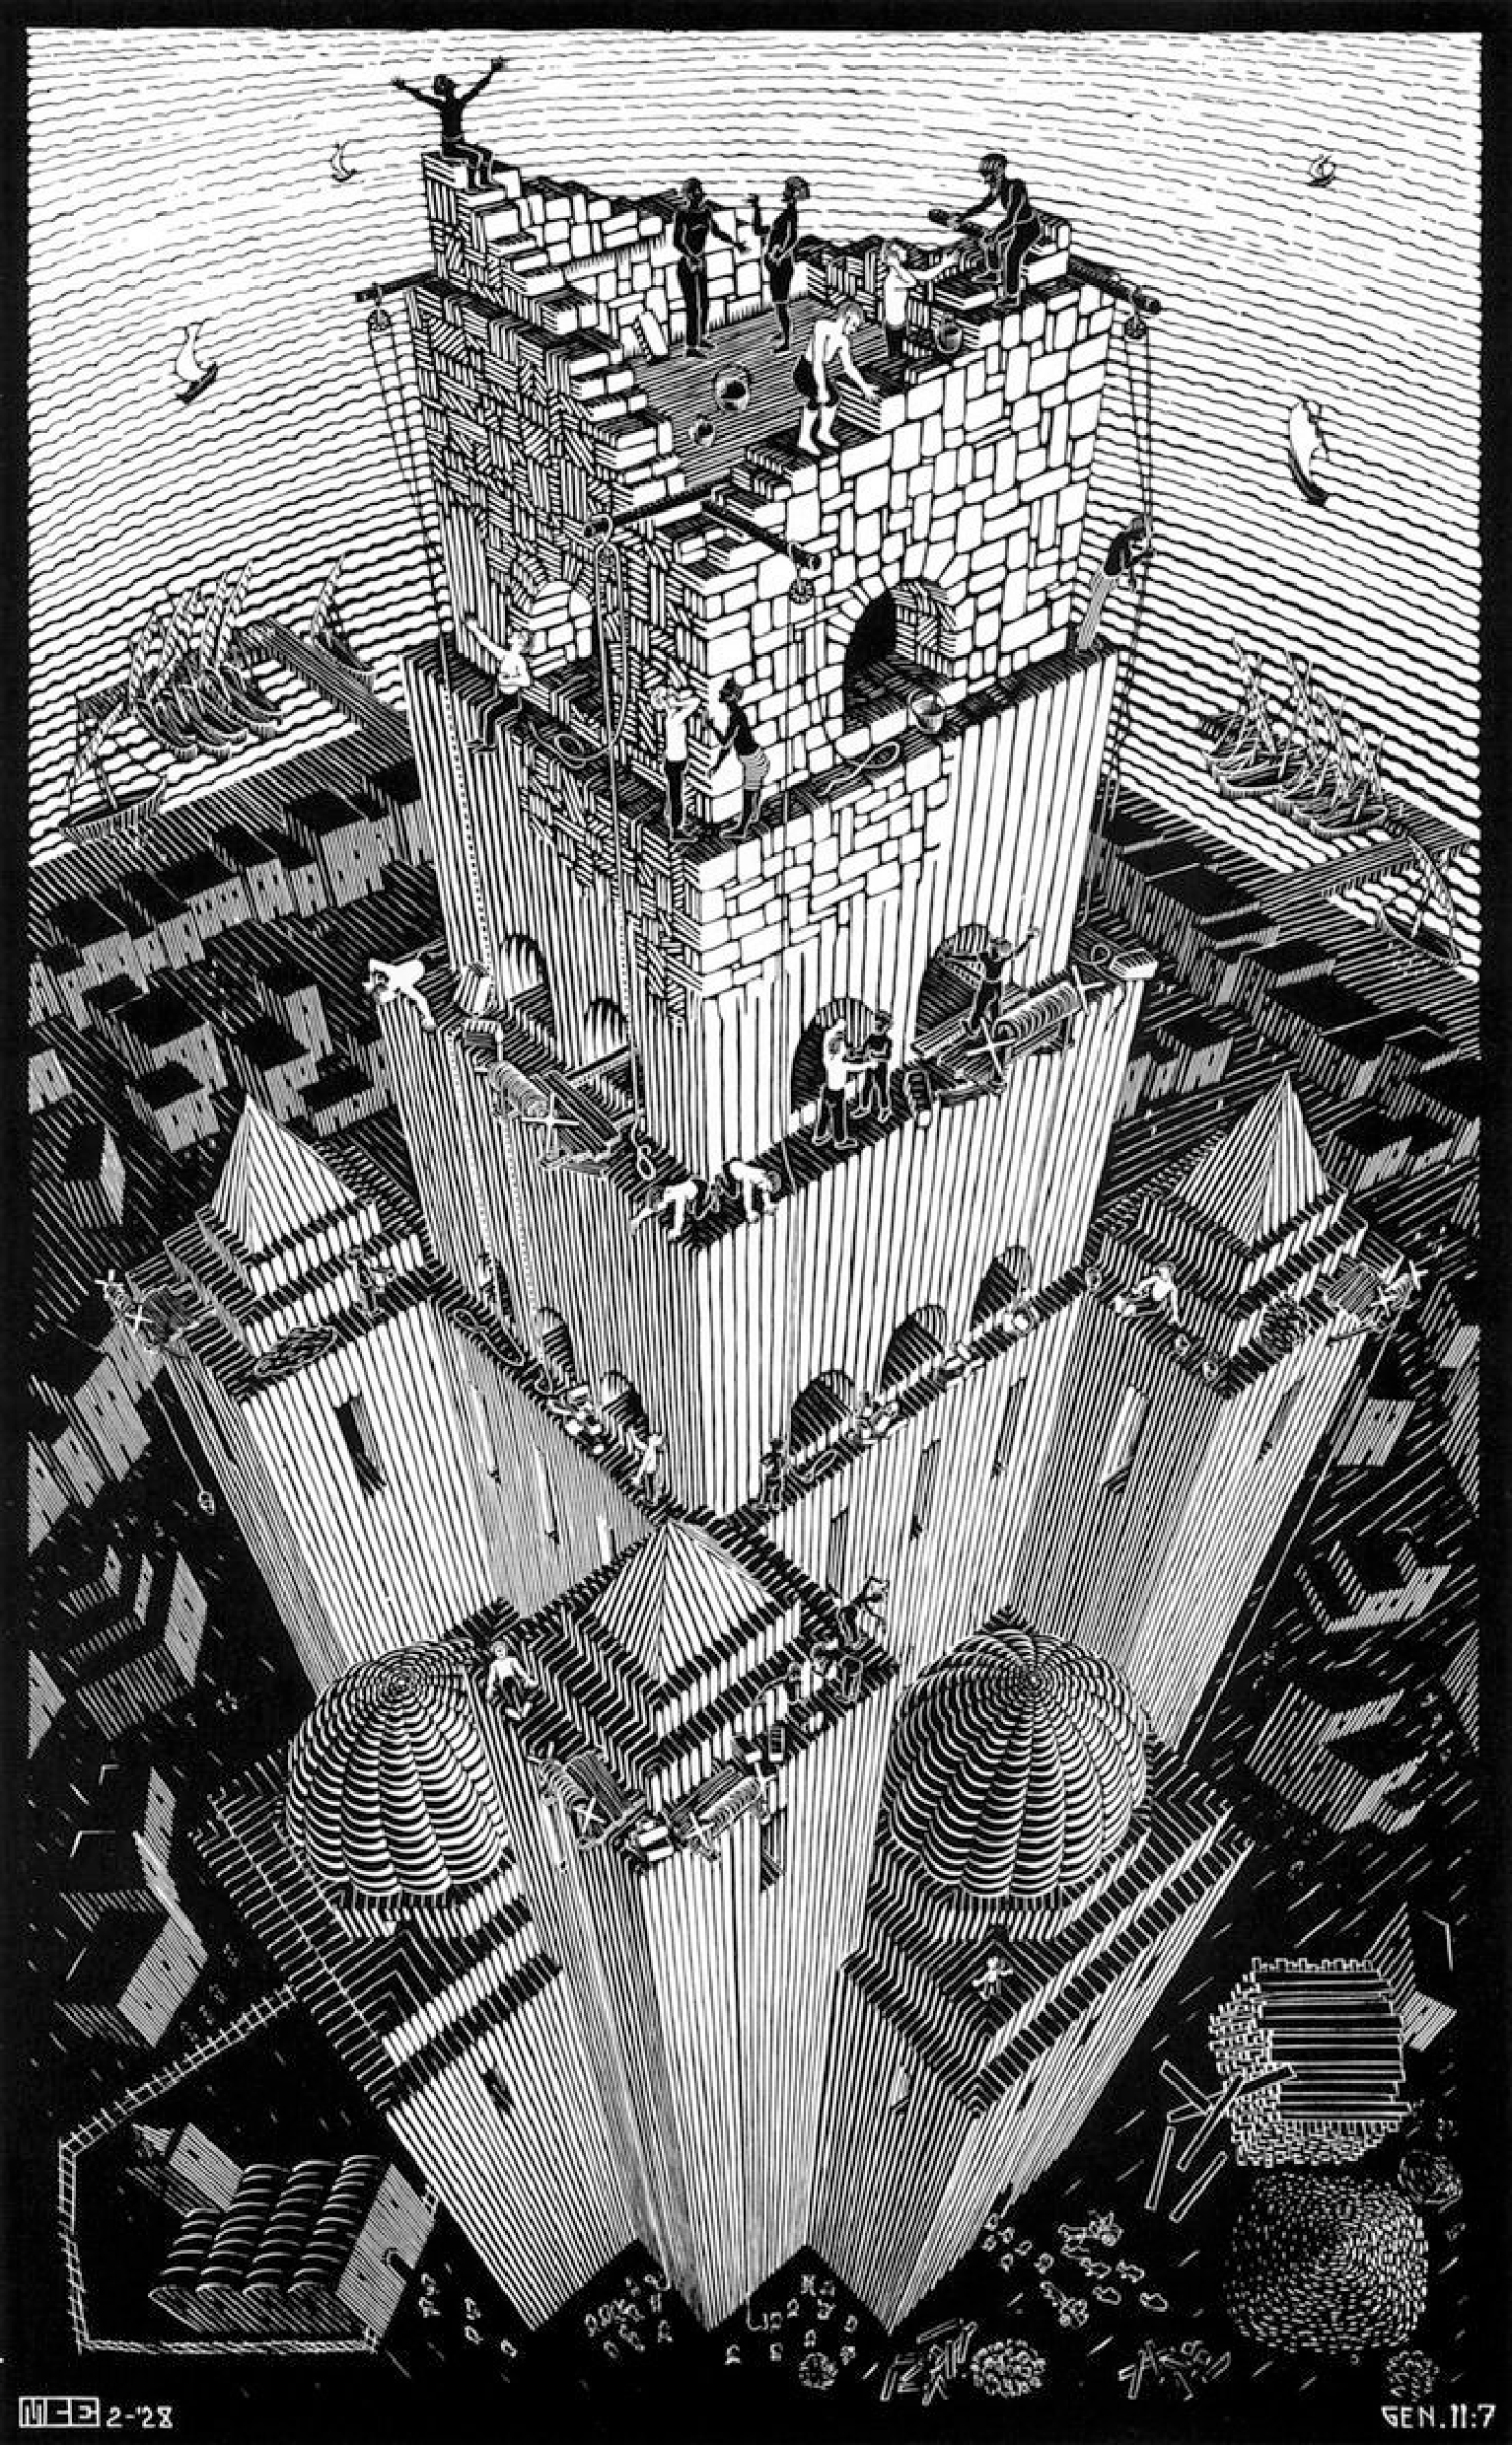
\includepdf[scale=.75]{escher_babel_2.pdf}
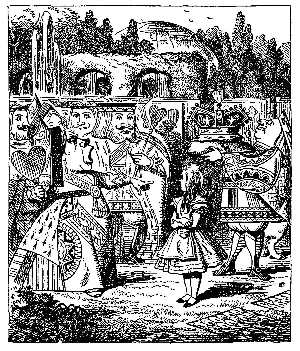
\includepdf[scale=.75]{alice_8.pdf}
% \includepdf[scale=.8]{escher_babel.pdf}
% \includepdf[scale=.7]{alice_2.pdf}
\chapter*{\hypertarget{chwiener}{\normalfont\textbf{Attacco di Wiener}}}
\chaptermark{Attacco di Wiener}
\addcontentsline{toc}{chapter}{Attacco di Wiener}

% Per velocizzare il calcolo della funzione di decifrazione, è spesso abitudine usare un'esponente privato piccolo $d$. Sfortunatemente, come vedremo in seguito, l'uso di un $d$ piccolo non è una buona idea e può portare ad una rottura totale del sistema $RSA$:
% \[
%   \{ e,n \}\, \overset{\mathcal{P}}{\longrightarrow}\, \{ d \text{ \scriptsize piccolo} \}
% \]
% Così detto, l'utilizzo di un $d$ piccolo, comporta problemi ben più seri dell'utilizzo di un $e$ piccolo in un sistema $RSA$. Questo perchè $d$ è più importante di qualsiasi altro componente della funzione \textit{One-Way Trapdoor} $\bigl(d,p,q,\phi(n)\bigr)$.

% --------------------------------------------------------------------------------

% Per velocizzare la cifratura e decifrazione dell'$RSA$, è possibile usare esponenti pubblici e segrti piccoli. La scelyta di un piccolo $e$ o $d$, è interessante soprattutto quando c'è una grande differenza in potenza di calcolo tra due dispositivi comunicanti, come tra una samrtcard e un computer.

% Nul 1990 Wiener descrive un attacco all'$RSA$ con esponente privato piccolo. Egli mostra che se $d{<}n^{0.25}$ allora $d$ è il denominatore di alcuni convergenti dell'espansione  in frazione continua di $\frac{e}{n}$, quindi $d$ può essere calcolato efficientemente dalla chiave pubblica $(n,e)$.

% I suoi risultati sono basati sul classico teorema di Legendre sulle approssimazioni diofantee della forma $|\alpha{-}\frac{a}{b}|{<}\frac{1}{2b^2}$

% --------------------------------------------------------------------------------

% \`E sempre preferibile avere una chiave privata di decifrazione $d$ relativamente piccola, che permetta un basso tempo di decifrazione, specialmente per dispositivi a bassa potenza di calcolo come la smartcard. Sfortunatamente, il seguente attacco suggerito da Wiener più di 20 anni fa, dimostra che scegliere un piccolo valore $d$, risulta in un sistema altamente insicuro ove tutte le informazioni segrete possono essere recuperate.

% L'attacco di Wiener dimostra la mancanza di sicurezza in un sistema dove $d$ è scelto tale che $d{\leq}n^{0.25}$. Usa un semplice algoritmo basato sulla fraziuoni continue che trova il numeratore e denominatore di una frazione in tempo polinomiale, quando è conosciuta una stima sufficientemente precisa della frazione.

% Nel contesto dell'$RSA$ possiamo usare l'esponente pubblico $e$ ed il modulo $n$ per creare una frazione ``approssimata'' che coinvolga l'esponente segreto $d$. Questo semplice algoritmo per fattorizzare il modulo può essere applicato quando $e{<}n$, $MCD(p{-}1,q{-}1)$ è piccolo, $p$ e $q$ hanno approssimativamente lo stesso numero di bits.

Per velocizzare il calcolo della funzione di decifrazione $Dec_k$,\mnote{
  \begin{definizione}[\textsc{Frazione Continua}]\
  
    Una frazione continua finita è una espressione della forma
    \begin{equation*}
      \gamma=
      \beta_0+\cfrac{\alpha_1}{\beta_1+\cfrac{\alpha_2}{\raisebox{0.5\height}{$\ddots$}+\cfrac{\alpha_{n-1}}{\beta_{n-1}+\cfrac{\alpha_n}{\beta_n}}}}
    \end{equation*}
    con $\alpha_i$, $\beta_i$ ($i{=}1{\dots}n{\in}\mathbb{Z}\SP{+}$) detti numeratori e denominatori parziali, $\gamma$ valore.\
    
    La frazione è chiamata \textbf{regolare} se $\beta_0{\in}\mathbb{Z}$, $\alpha_i{=}1$, $\beta_i{\in}\mathbb{Z}\textsuperscript{+}$ ($i{=}1{\dots}n$). Una frazione regolare sarà dunque esprimibile come sequenza dei propri denominatori parziali:
    \[
      \gamma = \bigl[\ \beta_0;\ \beta_1,\ \beta_2,\ \dots\ ,\beta_n\ \bigr]
    \]
  \end{definizione}

  \begin{definizione}[\textsc{Convergente}]\
    
    \label{convergente}
    Per $0{\leq}i{\leq}n$, si definisce i-esimo convergente di $\gamma$ la frazione $c_i{=}[\beta_0;\beta_1,\beta_2,\dots,\beta_i]$.
    % \[
    %   c_i = \bigl[\ \beta_0;\ \beta_1,\ \beta_2,\ \dots\ ,\beta_i\ \bigr]
    % \]
  \end{definizione}
}è abitudine usare un esponente privato $d$ piccolo, soprattutto in dispositivi dalle risorse limitate come le smartcards. Sfortunatamente però un attacco suggerito da Michael Wiener nel 1989 \cite{wiener}, basato sulle \textit{frazioni continue}, dimostra che scegliere $d$ piccolo, comporta un sistema altamente insicuro dove tutte le informazioni segrete possono essere recuperate. In particolare:
\[
  % (e,n)\, \overset{\mathcal{P}}{\Longrightarrow}\, \{ d \text{ \scriptsize piccolo} \}
  (e,N)\, \xrightarrow[\ d \text{ \scriptsize piccolo}\ ]{\mathcal{P}}\, \{ d \}
\]
Usando il \textit{Teorema di Legendre} sulle approssimazioni diofantee della forma $|\gamma{-}\frac{a}{b}|{<}\frac{1}{2b^2}$, l'Attacco mostra che se $d{<}\sqrt[4]{N}$, i convergenti dell'espansione in frazione continua di $\nicefrac{e}{N}$ (che ne approssimano il valore), sono della forma $\nicefrac{k}{d}$.
% $\text{(con $k{\in}\mathbb{Z}$)}$.

Quindi è immediato che $d$ possa essere calcolato efficientemente a partire dalla chiave pubblica $(e,N)$.\marginnote[11pt]{
  \begin{changemargin}{0.1cm}{-0.4cm}
    \setlength{\parindent}{1.5ex}
    % Si noti che, come da standard (PKCS $\#1$), si assumeranno gli esponenti pubblico e privato inversi modulo $\lambda(n)$, Funzione di Carmichael:
    Si ricordi che, come previsto nel \textit{PKCS $\#1$}, gli esponenti $e,d$, sono inversi in $\mathbb{Z}^*_{\lambda(N)}$:
    \[
      % \begin{array}{l}
        0 < k = \frac{ed-1}{\lambda(N)} < \frac{ed}{\lambda(N)} < min\{ e,d \}
        % \hspace{0pt}\text{\scriptsize quindi } k{<}d
      % \end{array}
    \]
    Le specifiche \hypertarget{pkcs1}{\textbf{\textit{PKCS}}} (Public Key Cryptography Standards), attualmente prodotte dagli RSA-Laboratories in collaborazione con esperti di sicurezza di tutto il mondo, hanno l'obiettivo di accelerare lo sviluppo della crittografia a chiave pubblica. \par
    Pubblicate nel 1991 ad un incontro dei primi utilizzatori delle tecnologie a chiave pubblica, sono divenute un importante ed aggiornato riferimento per chiunque.
    Tra i moderni standard che fanno uso delle \textit{PKCS} si ricordano
    % \textit{ANSI X9}, \textit{IEEE P1363},
    \textit{SSL/TLS} e \textit{WAP/WTLS}. \par
    Nello specifico, la famiglia delle \textit{PKCS $\#1$} fornisce definizioni di base e accorgimenti di sicurezza per l'implementazione del crittosistema $RSA$. \cite{pkcs}
  \end{changemargin}
}

\section*{\normalfont\textbf{Il ruolo dei convergenti}} %il ruolo dei convergenti
\addcontentsline{toc}{section}{Il ruolo dei convergenti}

I convergenti di una frazione continua regolare sono strettamente correlati al suo valore $\gamma$ e giocano un ruolo fondamentale nell' Attacco di Wiener. Dunque, come calcolarli?

\begin{thm}
  \label{convergenti}
  Data la frazione continua regolare
  \begin{equation*}
    \gamma =
    \beta_0+\cfrac{1}{\beta_1+\cfrac{1}{\raisebox{0.5\height}{$\ddots$}+\cfrac{1}{\beta_{n-1}+\cfrac{1}{\beta_n}}}} = \bigl[\ \beta_0;\ \beta_1,\ \dots\ ,\beta_{n-1},\ \beta_n\ \bigr]
  \end{equation*}
  e definiti due interi positivi $a_i$, $b_i$ ($i{=}{-}1{\dots}n$) tali che
  
  \begin{minipage}[b]{0.45\linewidth}
    \center
    \[
      \hspace{-5pt}a_i {=}
      \begin{cases}
        1 &\text{\scriptsize se } i{=}{-}1\\
        \beta_0 &\text{\scriptsize se } i{=}0\\
        \beta_i a_{i-1}{+}a_{i-2} &\text{\scriptsize se } 1{\leq}i{\leq}n
      \end{cases}
    \]
  \end{minipage}
  \begin{minipage}[b]{0.45\linewidth}
    \center
    \[
      \hspace{5pt}b_i {=}
      \begin{cases}
        0 &\text{\scriptsize se } i{=}{-}1\\
        1 &\text{\scriptsize se } i{=}0\\
        \beta_i b_{i-1}{+}b_{i-2} &\text{\scriptsize se } 1{\leq}i{\leq}n
      \end{cases}
    \]
  \end{minipage}

  \newpage
  \noindent
  l'i-esimo convergente $c_i$ può essere calcolato ricorsivamente:\mnote{
    \begin{lem}
      \label{lemma4}
      % I convergenti di indice pari ($c_{2k}$) incrementano stre
      % La successione dei convergenti $\{ c_i \}_{\tiny\substack{\hspace{-3pt}i{=}2k\\k{\in}\mathbb{Z}\SP{+}}}$ è monotona strettamente crescente, $\{ c_i \}_{\tiny\substack{i{=}2k{+}1\\\hspace{-4pt}k{\in}\mathbb{Z}\SP{+}}}$ è monotona strettamente decrescente.
      Sia $k{\in}\mathbb{Z}\SP{+}$. La successione dei convergenti pari $\{ c_i \}_{\scalebox{0.7}{$i{=}2k$}}$ è monotona strettamente crescente, mentre la $\{ c_i \}_{\scalebox{0.7}{$i{=}2k{+}1$}}$ dei dispari è monotona strettamente decrescente.
    \end{lem}
    \begin{proof}
      Partendo da (\ref{eq_minimi_termini}) e usando $a_i$, $b_i$ definiti in (\ref{eq_convergente}), posso ottenere la seguente uguaglianza:
      \[
        \begin{array}{c}
          a_ib_{i-2}{-}a_{i-2}b_i=({-}1)^i\beta_i\\
          \text{
            \begin{minipage}[c]{0.2\linewidth}
              \tiny
              e se divido\\
              per $b_ib_{i-2}$
            \end{minipage}
            \begin{minipage}[c]{0.55\linewidth}
              $c_i{-}c_{i-2}=({-}1)^i\frac{\beta_i}{b_ib_{i-2}}$
            \end{minipage}
          }
        \end{array}
      \]
      % Quindi è immediato concludere che $c_i{-}c_{i-2}$ ha segno $({-}1)^i$ e questo prova la tesi.
      Quindi la differenza tra due convergenti dispari (pari) consecutivi avrà sempre segno negativo (positivo).
    \end{proof}
  
    \begin{lem}
      \label{lemma5}
      % Ogni convergente dispari è maggiore di un qualsiasi convergente pari.
      Ogni convergente $c{\in}\{ c_i \}_{\scalebox{0.7}{$i{=}2k{+}1$}}$ è maggiorante di $\{ c_i \}_{\scalebox{0.7}{$i{=}2k$}}$.
    \end{lem}
    \begin{proof}
      Analogamente alla precedente, dividendo per ${-}b_ib_{i{-}1}$ entrambi i membri di (\ref{eq_minimi_termini}), si ottiene:
      \[
        \begin{array}{c}
          c_i{-}c_{i-1} = \frac{({-}1)^{i-1}}{b_ib_{i-1}}
        \end{array}
      \]
      Segue che la differenza tra due convergenti consecutivi $c_i$ e $c_{i-1}$ avrà sempre segno $({-}1)^{i-1}$. Quindi, per $\mu{\in}\mathbb{Z}\SP{+}$:
      \begin{equation}
        \label{conv_consecutivi}
        c_{2\mu+1} > c_{2\mu}
      \end{equation}
      Se, per assurdo, la tesi fosse falsa, dati $\mu,\eta{\in}\mathbb{Z}\SP{+}$, risulterebbe:
      \[
        c_{2\mu+1}{\leq}c_{2\eta} \Rightarrow
        \begin{cases}
          c_{2\mu+1}{<}c_{2\mu} &\text{\scriptsize se } \eta{<}\mu\\
          c_{2\eta+1}{<}c_{2\eta} &\text{\scriptsize se } \eta{>}\mu
        \end{cases}
      \]
      in contraddizione con (\ref{conv_consecutivi}).
    \end{proof}
  
    \begin{lem}
      \label{lemma6}
      $\gamma$ è maggiorante di $\{ c_i \}_{\scalebox{0.7}{$i{=}2k$}}$ e minorante di $\{ c_i \}_{\scalebox{0.7}{$i{=}2k{+}1$}}$.
    \end{lem}
    \begin{proof}
      $\gamma{=}c_n$, per qualsiasi valore di $n$, risulterà il maggiore dei convergenti pari, o il minore di quelli dispari: la tesi sarà vera in entrambi i casi.
    \end{proof}
  }
  \begin{equation}
    \label{eq_convergente}
    c_i = \frac{a_i}{b_i} = \frac{\beta_i a_{i-1}{+}a_{i-2}}{\beta_i b_{i-1}{+}b_{i-2}}
  \end{equation}
\end{thm}

\begin{proof}
  Procedendo per induzione, il passo base ($i{=}1$) risulta:
  \[
    c_1 = \frac{a_1}{b_1} = \beta_0{+}\frac{1}{\beta_1} = \frac{\beta_0\beta_1{+}1}{\beta_1} = \frac{\beta_1a_0{+}a_{-1}}{\beta_1b_0{+}b_{-1}}
  \]
  mentre il passo induttivo ($i{\Rightarrow}i{+}1$) è verificabile osservando che il convergente $c_{i+1}$ può essere costruito da $c_i$ sostituendo $\beta_i$ con $\beta_i{+}\frac{1}{\beta_{i+1}}$:
  \[
    \begin{split}
      c_{i+1} &= \frac{a_{i+1}}{b_{i+1}} = \frac{\bigl(\beta_i{+}\frac{1}{\beta_{i+1}}\bigr)a_{i-1}{+}a_{i-2}}{\bigl(\beta_i{+}\frac{1}{\beta_{i+1}}\bigr)b_{i-1}{+}b_{i-2}}
      = \frac{{\color{red}\overset{a_i}{\boxed{\color{black}\beta_ia_{i-1}{+}a_{i-2}}}}{+}\frac{a_{i-1}}{\beta_{i+1}}}{{\color{red}\underset{b_i}{\boxed{\color{black}\beta_ib_{i-1}{+}b_{i-2}}}}{+}\frac{b_{i-1}}{\beta_{i+1}}}=\\
      &= \frac{a_i{+}\frac{a_{i-1}}{\beta_{i+1}}}{b_i{+}\frac{b_{i-1}}{\beta_{i+1}}} = \frac{\beta_{i+1}a_i{+}a_{i-1}}{\beta_{i+1}b_i{+}b_{i-1}}
    \end{split}
  \]
\end{proof}

\noindent
Il Teorema \ref{convergenti} suggerisce dunque come approssimare una frazione continua regolare con un numero razionale e fornisce un semplice algoritmo per calcolarne i convergenti; chi ci assicura però che questi siano già ridotti ai minimi termini?

\begin{lem}
  \label{minimi-termini}
  Gli interi $a_i$, $b_i$ definiti nel Teorema \ref{convergenti} soddisfano
  \begin{equation}
    \label{eq_minimi_termini}
    a_{i-1}b_i {-} a_ib_{i-1} = (-1)^i
  \end{equation}
\end{lem}
\begin{proof}
  % Passo base ($i{=}0$):\, $a_{-1}b_0 - a_0b_{-1} = (-1)^0$\\
  % Passo induttivo ($i{\Rightarrow}i{+}1$): $a_ib_{i+1}{-}a_{i+1}b_i{=}$
  % \hfill---
  % \begin{description}[nosep, leftmargin=.25in, labelindent=0in]
  %   \item[\normalfont{($i{=}0$)}] $a_{-1}b_0{-}a_0b_{-1} = (-1)^0$
  %   \item[\normalfont{($i{\Rightarrow}i{+}1$)}]
  %   $a_ib_{i+1}{-}a_{i+1}b_i = a_i(b_i\beta_{i+1}{+}b_{i-1}){-}(a_i\beta_{i+1}{+}a_{i-1})b_i=$\\
  %   $\text{\hspace{84pt}}= -(a_{i-1}b_i{-}a_ib_{i-1}) = (-1)^{i+1}$
  % \end{description}
  \[
    \begin{array}{l}
      \text{(} i{=}0 \text{)}\quad a_{-1}b_0{-}a_0b_{-1} = (-1)^0\\
      \begin{split}
        \text{(} i{\Rightarrow}i{+}1 \text{)}\quad a_ib_{i+1}{-}a_{i+1}b_i &= a_i(b_i\beta_{i+1}{+}b_{i-1}){-}(a_i\beta_{i+1}{+}a_{i-1})b_i=\\
                                                       &= -(a_{i-1}b_i{-}a_ib_{i-1}) = (-1)^{i+1}
      \end{split}
    \end{array}
  \]
\end{proof}
\marginnote[-1pt]{ %-11pt se si sposta troppo
  \begin{changemargin}{0.1cm}{-0.4cm}
    \setlength{\parindent}{1.5ex}
    I Lemmi \ref{lemma4}, \ref{lemma5}, \ref{lemma6} mostrano che $\gamma$ di una frazione continua finita regolare è equivalente ad un numero razionale ed i suoi convergenti ne sono un'approssimazione. Ai fini dell'Attacco però è utile sapere il viceversa: \textbf{\textit{un numero razionale \boldmath$\nicefrac{x}{y}$ è esprimibile come una frazione continua finita regolare}}. \par
    La dimostrazione è piuttosto semplice e, come accennato, ruota attorno all'Algoritmo di Euclide esteso: trovato $MCD(x,y)$, si divide ciascuna equazione dell'algorirmo per il resto al passo precedente, così da individuare razionali espressi come somma di un intero e un razionale; fatto ciò, tramite eliminazioni successive, è immediato ottenere $\nicefrac{x}{y}$ nella forma desiderata.
  \end{changemargin}
}

\noindent
Dal Lemma \ref{minimi-termini} segue quindi che tutti i convergenti $c_i$ ($i{=}0{\dots}n$) sono ridotti ai minimi termini perchè $MCD(a_i,b_i){>}1$ appare sicuramente come divisore di $a_{i-1}b_i{-}a_ib_{i-1}$.

\addcontentsline{toc}{subsection}{Approssimare $\gamma$}
\paragraph{\normalfont\textbf{\underline{Approssimare $\gamma$.}}}Nella teoria generale, uno dei motivi d'importanza della rappresentazione dei numeri mediante frazioni continue risiede nel fatto che i relativi convergenti forniscono la migliore approssimazione possibile di un irrazionale mediante razionali. Benchè interessante, per i nostri scopi la rappresentazione di irrazionali non è rilevante ma i risultati generali possono essere usati anche per lo sviluppo in frazioni continue di razionali.
\begin{thm}
  \label{legendre1}
  Sia $a,b{\in}\mathbb{Z}\SP{+}$, $\gamma{=}[\beta_0;\beta_1,\dots,\beta_n,\beta_{n+1},\dots]$ frazione continua regolare\sidenote[2][]{} e $\{ c_i \}_{\scalebox{.7}{$i{\in}\mathbb{N}$}}$ l'insieme dei convergenti di $\gamma$. Se
  \begin{equation}
    \label{legendre1-1}
    |\gamma b{-}a| < |\gamma b_n{-}a_n|
  \end{equation}
  allora $b{\geq}b_{n+1}$. Inoltre, se
  \begin{equation}
    \label{legendre1-2}
    \Bigl|\gamma {-}\frac{a}{b}\Bigr| < |\gamma {-}c_n|
  \end{equation}
  allora $b{>}b_n$. In altri termini ogni convergente $c_n{=}\nicefrac{a_n}{b_n}$ approssima $\gamma$ meglio di qualunque frazione il cui denominatore non superi $b_n$.
\end{thm}
\begin{proof}
  Data l'ipotesi (\ref{legendre1-1}), supponendo per assurdo $b{<}b_{n+1}$, si consideri la seguente implicazione per qualche $x,y{\in}\mathbb{Z}$:
  
  % \begin{marginfigure}[14pt]
  %   \center
  %   \includegraphics[width=\textwidth]{snoopy_square.png}
  % \end{marginfigure}
  % \bigskip
  % \vspace{-0.1cm}
  \hspace{-10pt}\begin{minipage}[b]{0.45\linewidth}
    \[
      \begin{cases}
        a_nx {+} a_{n+1}y = a\\
        b_nx {+} b_{n+1}y = b
      \end{cases}
    \]
  \end{minipage}
  \begin{minipage}[b]{0.45\linewidth}
    \[
      \hypersetup{linkcolor=red}
      \hspace{-30pt}{\color{red} \underset{\text{(\ref{eq_minimi_termini})}}{\boxed{\color{black} \Longrightarrow}}}\hspace{5pt}
      \begin{cases}
        x = ({-}1)^n (a_{n+1}b{-}ab_{n+1})\\
        y = ({-}1)^n (ab_n{-}a_nb)
      \end{cases}
    \]
  \end{minipage}

  \hspace{-5pt}\begin{minipage}[b]{0.1\linewidth}
    \scriptsize
    con $x,y$\\
    tali che
  \end{minipage}
  \begin{minipage}[b]{0.45\linewidth}
    \[
      \begin{split}
        & x {\neq} 0\ \xrightarrow{\ altrimenti\ }\ b {=} b_{n+1}y {\geq} b_{n+1}\\
        & y {\neq} 0\ \xrightarrow{\ altrimenti\ }\, {\scriptsize \begin{cases}
            a {=} a_nx\\
            b {=} b_nx
          \end{cases}} \hspace{-5pt}\Rightarrow |\gamma b{-}a| {=} |x||\gamma b_n{-}a_n|{\geq}|\gamma b_n{-}a_n|
      \end{split}
    \]
  \end{minipage}

  \bigskip
  \noindent
  Inoltre è utile dimostrare che $x$ e $y$ hanno effettivamente segni opposti:
  \[
    \begin{split}
      & \text{\scriptsize se}\, y{<}0\ \Longrightarrow\ b_nx{=}b{-}b_{n+1}y{>}0 \hspace{3pt} {\color{red}\overset{b_n{>}0}{\boxed{\color{black}\Rightarrow}}} \hspace{3pt} x{>}0\\
      & \text{\scriptsize se}\, y{>}0\ \Longrightarrow\ b_nx{=}b{-}b_{n+1}y{<}0 \hspace{-14pt} {\color{red}\underset{b_{n+1}y{\geq}b_{n+1}{>}b}{\boxed{\color{black}\Rightarrow}}} \hspace{-14pt} x{<}0
    \end{split}
  \]
  Adesso, dall'andamento oscillante dei convergenti mostrato nei Lemmi \ref{lemma4}, \ref{lemma5} segue subito che $\gamma b_n{-}a_n$ e $\gamma b_{n+1}{-}a_{n+1}$ hanno segni opposti; pertanto $x(\gamma b_n{-}a_n)$ e $y(\gamma b_{n+1}{-}a_{n+1})$ hanno lo stesso segno. Quindi si può concludere:
  \[
    \begin{split}
      |\gamma b{-}a| & = |\gamma(b_nx{+}b_{n+1}y)-(a_nx{+}a_{n+1}y)|\\
      & = |x||\gamma b_n{-}a_n| + |y||\gamma b_{n+1}{-}a_{n+1}|\\
      & \geq |\gamma b_n{-}a_n|
    \end{split}
  \]
  che però nega l'ipotesi (\ref{legendre1-1}). Questo dimostra la prima tesi del teorema. Presa ora in considerazione l'ipotesi (\ref{legendre1-2}) e supposto per assurdo $b{\leq}b_n$, troviamo nuovamente l'ipotesi (\ref{legendre1-1}):
  \[
    b\Bigl| \gamma {-}\frac{a}{b} \Bigr| < b_n|\gamma {-}c_n|
  \]
  Questo suggerisce $b_n{\geq}b{\geq}b_{n+1}$ che però contraddice (\ref{eq_convergente}).
  % che quindi suggerisce $b_n{\geq}b{\geq}b_{n+1}$, in cottraddizione però con (\ref{eq_convergente}).
  % $\scriptsize\begin{cases}
  %   x{\neq}0\\
  %   y{\neq}0
  % \end{cases}$, altrimenti si avrebbe $\scriptsize\begin{cases}
  %   b{=}b_{n+1}y{\geq}b_{n+1}\\
  %   b{=}b_{n+1}y{\geq}b_{n+1}
  % \end{cases}$, contro l'ipotesi. Similmente
\end{proof}\marginnote[-283pt]{\textbf{\textit{Nel calcolo di \boldmath$\sqrt{2}$ mediante convergenti, qual'è l'errore commesso?}}\par
Dall'espansione in frazione continua regolare si ottiene che $\sqrt{2}{=}[1;\overline{2}]$; quindi l'insieme dei convergenti risulterà:
\[
  \{ c_i \}_{\scalebox{.7}{$i{\in}\mathbb{N}$}} = \biggl\{ 1,\,\frac{3}{2},\,\frac{7}{5},\,\frac{17}{12},\,\frac{41}{29},\,\dots \biggr\}
\]
Scelto di approssimare $\sqrt{2}$ con $c_2{=}\nicefrac{7}{5}$, l'errore $\mathcal{E}$ che si commette è pari a $|\sqrt{2}{-}c_2|{<}\abs{c_3{-}c_2}{=}0.01\overline{6}$. Adesso, usando la tesi del Teorema \ref{legendre1}, è possibile mostrare che ogni frazione con denominatore minore di $5$ commette un errore maggiore di $\mathcal{E}$.

Considerato $1{<}\sqrt{2}{<}2$, l'insieme dei possibili razionali sarà $\{ \frac{5}{4},\frac{7}{4},\frac{4}{3},\frac{5}{3},\frac{3}{2} \}$, dal quale sono subito eliminabili $\nicefrac{5}{4}$ e $\nicefrac{4}{3}$ perchè minori di $c_2$, sottostima di $\sqrt{2}$. Successivamente è sufficiente mostrare che per il minore dei rimanenti ($\nicefrac{3}{2}$), vale la seguente disuguaglianza:
\[
  \Bigl|\sqrt{2}{-}\frac{3}{2}\Bigr| > \Bigl|\frac{3}{2}{-}c_2\Bigr| = 0.18\overline{3} > \mathcal{E}
\]
Quindi $\nicefrac{7}{5}$ è effettivamente la miglior approssimazione razionale di $\sqrt{2}$ con denominatore minore o uguale a $5$.}
% $|\sqrt{2}{-}c_2|{<}|\sqrt{2}{-}\frac{5}{4}|$ e $|\sqrt{2}{-}c_2|{<}|\sqrt{2}{-}\frac{4}{3}|$.}
% Adesso che le proprietà di base sono definite, un'ultima importante relazione è data dal Teorema di Legendre: esso rappresenta un fondamentale tassello nella dimostrazione dell'Attacco di Wiener.
\begin{thm}[\textsc{Legendre}]
  \label{legendre2}
  Sia $a,b{\in}\mathbb{Z}\SP{+}$, $\gamma{=}[\beta_0;\beta_1,\dots,\beta_n,\beta_{n+1},\dots]$ frazione continua regolare\sidenote[][-547pt]{Sono usate \textbf{frazioni continue infinite}. Queste hanno stessa struttura delle finite ma un numero infinito di denominatori parziali e sono molto utili per l'approssimazione di irrazionali.} e $\{ c_i \}_{\scalebox{.7}{$i{\in}\mathbb{N}$}}$ l'insieme dei convergenti di $\gamma$. Se
  \begin{equation}
    \label{legendre2-1}
    \Bigl|\gamma{-}\frac{a}{b}\Bigr| < \frac{1}{2b^2}
  \end{equation}
  allora $\frac{a}{b}{\in}\{ c_i \}_{\scalebox{.7}{$i{\in}\mathbb{N}$}}$.
\end{thm}
\begin{proof}
  Supponiamo per assurdo che $\frac{a}{b}{\notin}\{ c_i \}_{\scalebox{.7}{$i{\in}\mathbb{N}$}}$, sarà sempre possibile trovare due convergenti $c_n,c_{n+1}$ tali che $b_n{\leq}b{<}b_{n+1}$\sidenote[][]{
    La proposizione è facilmente verificabile: se per assurdo fosse falsa, tutti i convergenti avrebbero lo stesso denominatore ma questo è impossibile perchè contraddirebbe il Teorema \ref{convergenti}.
  }. Quindi, per il Teorema \ref{legendre1}:
  \[
    \begin{array}{c}
      |\gamma b_n{-}a_n| \leq |\gamma b{-}a| = b\bigl|\gamma {-}\frac{a}{b}\bigr| < \frac{1}{2b}\hspace{5pt} \Rightarrow\\
      \Rightarrow\hspace{5pt} |\gamma {-}c_n|<\frac{1}{2bb_n}
    \end{array}
  \]
  Poichè la tesi è negata per assurdo, $|a_nb{-}ab_n|{\geq}1$. Dunque:
  \[
    \begin{array}{c}
      \frac{1}{bb_n} \leq \frac{|a_nb{-}ab_n|}{bb_n} = \bigl|c_n{-}\frac{a}{b}\bigr| \leq |\gamma{-}c_n|{+}\bigl|\gamma{-}\frac{a}{b}\bigr| < \frac{1}{2bb_n}{+}\frac{1}{2b^2}\hspace{5pt} \Rightarrow\\
      \Rightarrow\hspace{5pt} \frac{1}{2bb_n} < \frac{1}{2b^2}
    \end{array}
  \]
  che implica $b_n{>}b$ contrario all'ipotesi.
\end{proof}

\noindent
Adesso che anche il Teorema di Legendre è stato definito, è finalmente possibile esporre il classico attacco alla chiave privata ideato da Wiener nel 1989; vedremo come la disuguaglianza (\ref{legendre2-1}) sia un fondamentale tassello nella dimostrazione dell'Attacco.

\section*{\normalfont\textbf{Attacco classico}} % Attacco originale
\addcontentsline{toc}{section}{Attacco classico}
\begin{marginfigure}[120pt] %120
  \center
  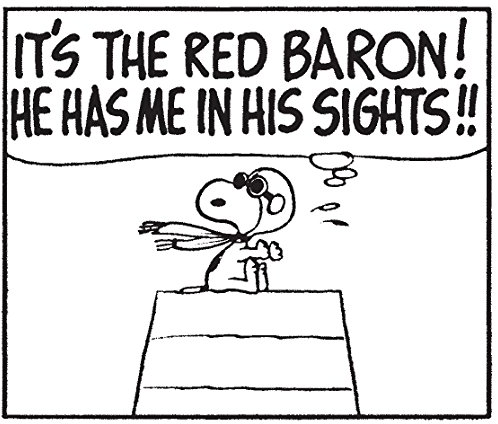
\includegraphics[width=\textwidth]{red_baron1.png}
  % \vspace{-10pt}
  % \caption{Se mostri il fianco al Barone Rosso.}
\end{marginfigure}
\marginnote[0pt]{
  \hspace{-2pt}\begin{minipage}[b]{0.45\textwidth}
    \captionof{figure}{Un classico attacco.}
    % \captionof{figure}{Mai offrire al Barone Rosso le condizioni per un Attacco!}
    % \captionof{figure}{Il Barone Rosso non perdona: mai offrire condizioni per un Attacco!}
  \end{minipage}
}
Come già introdotto all'inizio del capitolo, data semplicemente la chiave pubblica $(e,N)$, Wiener fattorizza il modulo $N$ usando le informazioni ottenute da uno dei convergenti nell'espansione di $\nicefrac{e}{N}$. Il miglior modo per procedere è dunque esprimere l'Attacco, nella sua forma più generale, con il seguente teorema.
\begin{thm}[\textsc{Wiener}]
  \label{th-wiener}
  Sia $N{=}pq$ un modulo $RSA$ e siano $e,d{\in}\mathbb{Z}^*_{\lambda(N)}$ i relativi esponenti pubblico e privato. Se $d$ soddisfa la seguente ipotesi:
  \begin{equation}
    \label{ip_wiener}
    d < \frac{pq}{2(p{+}q{-}1)k_0g_0} = \frac{N}{2\bigl(N{-}\phi(N)\bigr)k_0g_0}
  \end{equation}
  % Dati $k,g{\in}\mathbb{Z}\textsuperscript{+}$ tali che:
  % \[
  %   \begin{array}{l}
  %     k = \frac{ed{-}1}{\lambda(n)} = k_0\,MCD(k,g) \\
  %     g = MCD(p{-}1,q{-}1) = g_0\,MCD(k,g) \\
  %   \end{array}
  % \]
  \[
    \text{\footnotesize con}
    \hspace{12pt}{\footnotesize\begin{split}
      k &= k_0\,MCD(k,g) = \nicefrac{(ed{-}1)}{\lambda(N)} &\in \mathbb{Z}\textsuperscript{+}\\
      g &= g_0\,MCD(k,g) = MCD(p{-}1,q{-}1) &\in \mathbb{Z}\textsuperscript{+}\\
    \end{split}}
  \]
  % \begin{minipage}[b]{0.25\linewidth}
  %   \raggedleft
  %   con
  % \end{minipage}
  % \begin{minipage}[b]{0.6\linewidth}
  %   \[
  %     {\footnotesize\begin{split}
  %       k &= k_0\,MCD(k,g) = \nicefrac{(ed{-}1)}{\lambda(N)} &\in \mathbb{Z}\textsuperscript{+}\\
  %       g &= g_0\,MCD(k,g) = MCD(p{-}1,q{-}1) &\in \mathbb{Z}\textsuperscript{+}\\
  %     \end{split}}
  %   \]
  % \end{minipage}

  \medskip
  \noindent
  allora $N$ può essere fattorizzato in tempo polinomiale in $\mathcal{O}\bigl(log\P{2}(N)\bigr)$.
\end{thm}
\begin{proof}
  Usando una proprietà del massimo comun divisore\sidenote[][]{
    % $MCD(p{-}1,q{-}1)\,mcm(p{-}1,q{-}1){=}(p-1)(q-1)$
    Il prodotto di due interi $x,y$ è pari al prodotto del loro massimo comun divisore e minimo comune multiplo:
      \[
        xy = MCD(x,y)\,mcm(x,y)
      \]
    nel nostro caso $x{=}p{-}1$, $y{=}q{-}1$ e $\lambda(N)$ è il loro minimo comune multiplo.
  } è possibile riscrivere il prodotto dei due esponenti $ed$ come:

  % \begin{minipage}[b]{0.45\linewidth}
  %   \[
  %     \begin{cases}
  %       % \lambda(n) = \frac{(p{-}1)(q{-}1)}{MCD(p{-}1,q{-}1)}\\
  %       \phi(n) = g\lambda(n)\\
  %       ed = 1{+}k\lambda(n)
  %     \end{cases}
  %   \]
  % \end{minipage}
  % \begin{minipage}[b]{0.45\linewidth}
  %   \begin{equation}
  %     \Rightarrow\hspace{7pt} ed = 1{+}\frac{k}{g}\phi(n)
  %   \end{equation}
  % \end{minipage}
  \begin{equation}
    \label{sistema-ed}
    \begin{cases}
      \phi(N) = g\lambda(N)\\
      ed = 1{+}k\lambda(N)
    \end{cases}
    \Rightarrow\hspace{10pt} ed = 1{+}\frac{k}{g}\phi(N)
  \end{equation}

  \bigskip
  \noindent
  Adesso sarà sufficiente dividere entrambi i lati per $dN$ e usare l'ipotesi (\ref{ip_wiener}) per ottenere la seguente disuguaglianza:
  \begin{equation*}
    \abs{\frac{e}{N}{-}\frac{k_0}{dg_0}} = \abs{\frac{1}{dN}{-}\frac{k_0}{dg_0}\,\frac{N{-}\phi(N)}{N}} < \frac{k_0}{dg_0}\,\frac{N{-}\phi(N)}{N} < \frac{1}{2(dg_0)^2}
  \end{equation*}
  Come preannunciato, si noti l'assonanza tra l'ipotesi (\ref{legendre2-1}) del Teorema di Legendre e la disuguaglianza appena ricavata:

  % \begin{minipage}[b]{0.25\linewidth}
  %   \[
  %     \hspace{20pt}\abs{\gamma-\frac{a}{b}} < \frac{1}{2b^2} \hspace{10pt}
  %   \]
  % \end{minipage}
  % \begin{minipage}[b]{0.2\linewidth}
  %   \[
  %     \longrightarrow
  %   \]
  % \end{minipage}
  % \begin{minipage}[b]{0.25\linewidth}
  %   \[
  %     \abs{\frac{e}{n}-\frac{k_0}{dg_0}} < \frac{1}{2(dg_0)^2}
  %   \]
  % \end{minipage}
  \begin{equation}
    \label{disuguaglianza-wiener}
    \hspace{20pt}\abs{\gamma{-}\frac{a}{b}} < \frac{1}{2b^2}\hspace{10pt} \leftrightsquigarrow\hspace{8pt} \abs{\frac{e}{N}{-}\frac{k_0}{dg_0}} < \frac{1}{2(dg_0)^2}
  \end{equation}
  % \begin{marginfigure}[-15pt]
  %   \center
  %   \includegraphics[width=\textwidth]{snoopy_square.png}
  %   \vspace{-0.35cm}
  %   \caption{Chiaramente, in alcuni casi, l'attacco di Wiener è pleonastico!}
  % \end{marginfigure}
  
  \noindent
  Pertanto, per il Teorema \ref{legendre2}, \textbf{\boldmath$c{=}\frac{k_0}{dg_0}$ sarà uno degli \boldmath$n$ convergenti dell'espansione in frazione continua di \boldmath$\nicefrac{e}{N}$}. Usando (\ref{sistema-ed}), non rimane che calcolare $\phi(N)$ necessario per la fattorizzazione del modulo:\wwmnoteskip{-9pt}{\begin{description}[nosep, leftmargin=.39in, labelindent=0in]
    \item[\normalfont{\textbf{Input:}}] insieme $\{ c_i \}_{\scalebox{.7}{$i{\leq}n$}}$ dei convergenti dell'espansione di $\nicefrac{e}{N}$.
  \end{description}}\wmnoteskip{0pt}{
  % \hfill\rule{1\linewidth}{0.3pt}
    % \begin{algorithmic}[]
    %   \ttfamily
    %   \State $m \gets 0$
    %   \BState \textsc{Loop\textsubscript{$m$}:}
    %   \State $i \gets 0$
    %   \BState \textsc{Loop\textsubscript{$i$}:}
    %     \If{$(\frac{e}{c_i}{+}m) \Rightarrow IPF(n)$}
    %       \State \Return $c_i$
    %     \EndIf
    %     \If{$i{\leq}i_{max}$}
    %       \State $i \gets i{+}1$
    %       \State \textbf{jump} \emph{loop-i}
    %     \EndIf
    %     \If{$m{\leq}\lfloor \frac{g}{k} \rfloor$}
    %       \State $m \gets m{+}1$
    %       \State \textbf{jump} \emph{loop-m}
    %     \EndIf
    % \end{algorithmic}
    \begin{algorithmic}[]
      \fontfamily{qcr}\selectfont
      \State m$\gets$0
      \BState \textbf{LOOP\textsubscript{m}:}
      \State i$\gets$0
      \BState \textbf{LOOP\textsubscript{i}:}
        \If{$(\nicefrac{\text{e}}{\text{c\textsubscript{i}}}{-}\text{m}) \Rightarrow$IPF(n)}
          \State \Return c\textsubscript{i}
        \EndIf
        \If{i$\leq$n}
          \State i$\gets$i$+$1
          \State \textbf{goto} LOOP\textsubscript{i}
        \EndIf
        \If{m${\leq}\lfloor \nicefrac{\text{g}}{\text{k}} \rfloor$}
          \State m$\gets$m$+$1
          \State \textbf{goto} LOOP\textsubscript{m}
        \EndIf
      \end{algorithmic}}
      \wwmnoteskip{0pt}{\begin{description}[nosep, leftmargin=.48in, labelindent=0in]
        \item[\normalfont{\textbf{Output:}}] $i$-esimo convergente $c_i$, utile alla fattorizzazione di $N$.
      \end{description}}
      \marginnote[5pt]{
        \begin{minipage}[b]{0.49\textwidth}
          % \begin{changemargin}{0.1cm}{-0.4cm}
            % \scriptsize
            \captionof{figure}{Frammento di pseudocodice per la ricerca del corretto convergente.}
          % \end{changemargin}
        \end{minipage}
      }
  \begin{equation*}
    % \label{candidato}
    \phi(N)=e\,{\color{red} \underset{\nicefrac{b}{a}}{\boxed{\color{black}\frac{dg_0}{k_0}}} }-\frac{g_0}{k_0}=\biggl\lfloor \frac{e}{c}\biggr\rfloor {-} \biggl\lfloor \frac{g_0}{k_0} \biggr\rfloor
    % \underset{
    %   \text{
    %     \scalebox{0.95}{$\color{red}\rotatebox[origin=t]{150}{$=$}pippo$
    %   }}}{\color{red}\boxed{\color{black}\frac{dg_0}{k_0}}}
  \end{equation*}
  Questo garantisce la possibilità di calcolare $\phi(N)$ conoscendo il corretto convergente $c$, ovvero ricavare in tempo polinomiale $IFP(N)$ come mostrato nel Teorema \ref{ifp}.
    % Frammento di codice per la ricerca del corretto convergente.}
  I possibili candidati risulteranno dunque della forma $\lfloor\nicefrac{e}{c}\rfloor{-}m$. Fissato un intero $m$, sarà sufficiente iterare sulla lista dei convergenti e per ciascun candidato provare a fattorizzare il modulo $N$; se la ricerca fallisse, il processo verrà ripetuto con $m{+}1$.
  % In questo modo, abbiamo la certezza di calcolare il giusto candidato (\ref{candidato}) e fattorizzare $n$.

  Dal momento che la cardinalità di $\{ c_i \}_{\scalebox{.7}{$i{\leq}n$}}$ è polinomiale in $log\P{2}(N)$ e il valore di $m$ non può superare $\lfloor\nicefrac{g}{k}\rfloor$, il costo totale della ricerca avrà al più ordine $\Theta\bigl(log\P{2}(N)\bigr)$.
\end{proof}

\noindent
% \begin{fullwidth}
  \addcontentsline{toc}{subsection}{Analisi di efficienza}
  \paragraph{\normalfont\textbf{\underline{Analisi di efficienza.}}}Riguardo l'algoritmo descritto, benchè questo rispetti la tesi del Teorema \ref{th-wiener}, in certi casi è possibile ottimizzarne la resa riducendo la cardinalità dell'insieme $\{ c_i \}_{\scalebox{.7}{$i{\leq}n$}}$ in input.\mnoteskip{-27pt}{
    \begin{definizione}[\textsc{Primi Bilanciati}]\

    \label{primi-bilanciati}
    Con primi bilanciati si intendono due primi $p,q$ circa della stessa lunghezza binaria. In particolare, per un modulo $RSA$ $N{=}pq$ si assumerà che:
    \begin{equation*}
      4 < \frac{1}{2}\sqrt{N} < p < \sqrt{N} < q < 2\sqrt{N}
    \end{equation*}
    o equivalentemente che $p{<}q{<}2p$ come da \textit{Postulato di Bertrand}.
  \end{definizione}}
  \marginnote[3pt]{
    \begin{changemargin}{0.1cm}{-0.4cm}
      \setlength{\parindent}{1.5ex}
      Dalla Definizione \ref{primi-bilanciati} si può dunque inferire che, quando $p,q$ sono bilanciati, la funzione toziente di Eulero $\phi(N)$ soddisfi:
      \[
        \begin{split}
          |N{-}\phi(N)| &= |N{-}(p{-}1)(q{-}1)|\\
                        &= |p{+}q{-}1|\\
                        &< 3\sqrt{N}
        \end{split}
      \]
      Quindi $N$ e $\phi(N)$ avranno circa metà dei loro bit più significativi in comune. \par
      Una diretta conseguenza di quanto affermato è nuovamente la tesi del Postulato di Bertrand, ovvero $\phi(N){<}N{<}2\phi(N)$.
    \end{changemargin}}
  
  Nello specifico, tutti i convergenti $c_i$ per cui $|\nicefrac{e}{N}{-}c_i|$ non rispetta (\ref{disuguaglianza-wiener}), possono essere scartati a priori. Inoltre, se $p,q$ sono primi bilanciati scelti casualmente, la probabilità che $g$ sia piccolo è alta.
  \begin{table}
    % \phantomsection
    % \caption{pippo}
    \centering
    \begin{tabular}{cccccccc}
      % \hline
      \specialrule{.1em}{.05em}{.05em}
      % \hfill\rule{1\linewidth}{1pt}
      \rowcolor[gray]{.9}               &  \multicolumn{5}{c}{\textbf{Lunghezza binaria $p,q$}}  &  &  \\
      \rowcolor[gray]{.9}\textbf{g}     &  \textbf{128}    &  \textbf{256}    &  \textbf{384}    &  \textbf{512}  &  \textbf{1024}  &  \textbf{Media}  &  \textbf{Percentile}  \\\specialrule{.1em}{.05em}{.05em}
                         $2$            &  $49.5$          &  $49.7$          &  $49.8$          &  $49.5$        &  $49.5$         &  $49.6$          &  $49.6$               \\\hline
                         $4$            &  $12.4$          &  $12.4$          &  $12.4$          &  $12.3$        &  $12.4$         &  $12.4$          &  $62.0$               \\\hline
                         $6$            &  $14.7$          &  $14.6$          &  $14.6$          &  $14.7$        &  $14.8$         &  $14.7$          &  $76.7$               \\\hline
                         $8$            &  $3.1$           &  $3.1$           &  $3.0$           &  $3.2$         &  $3.2$          &  $3.1$           &  $79.8$               \\\hline
                         $10$           &  $3.1$           &  $3.2$           &  $3.1$           &  $3.2$         &  $3.1$          &  $3.2$           &  $83.0$               \\\hline
                         $12$           &  $3.8$           &  $3.5$           &  $3.6$           &  $3.5$         &  $3.6$          &  $3.6$           &  $86.6$               \\\hline
                         $14$           &  $1.4$           &  $1.3$           &  $1.4$           &  $1.3$         &  $1.4$          &  $1.4$           &  $88.0$               \\\hline
                         $16$           &  $0.7$           &  $0.7$           &  $0.8$           &  $0.8$         &  $0.8$          &  $0.8$           &  $88.8$               \\\hline
                         $18$           &  $1.6$           &  $1.6$           &  $1.6$           &  $1.7$         &  $1.6$          &  $1.6$           &  $90.4$               \\\hline
                         $20$           &  $0.7$           &  $0.7$           &  $0.8$           &  $0.8$         &  $0.8$          &  $0.8$           &  $91.2$               \\\specialrule{.1em}{.05em}{.05em}
                         \arrayrulecolor{white}\specialrule{.16em}{.09em}{.09em}
      % \multicolumn{8}{l}{\scriptsize Distribuzione di $g{=}MCD(p{-}1,q{-}1)$ per primi $p,q$ casuali, della stessa lunghezza.}
      \multicolumn{8}{l}{\scriptsize \begin{tabular}{@{}l@{}}Distribuzione di probabilità di $g{=}MCD(p{-}1,q{-}1)$ per primi $p,q$ casuali, della stessa\\lunghezza. I risultati sono dati in percentuale e comprendono i percentili totali.\end{tabular}}
    \end{tabular}
  \end{table}
  
  \bigskip
  \noindent
    Per esempio $\mathsf{Prob[}g{\leq}6\mathsf{]}\hspace{1pt}{\simeq}\hspace{1pt}0.77$ e addirittura $\mathsf{Prob[}g{\leq}20\mathsf{]}\hspace{1pt}{\simeq}\hspace{1pt}0.91$; pertanto è plausibile supporre $\lfloor \nicefrac{g}{k} \rfloor{=}0$ e, di conseguenza, la necessità di una sola\marginnote[-3pt]{
      \begin{changemargin}{0.1cm}{-0.4cm}
        \setlength{\parindent}{1.5ex}
        Data la chiave pubblica di una istanza di $RSA$ con esponente privato piccolo:
        \[ (e,N) = (58549809,2447482909) \]
        l'espansione di $\nicefrac{e}{N}$ ed il relativo insieme di convergenti risulteranno:
        % \[
        %   \begin{split}
        %     \frac{e}{N} &= [0;41,1,4,23,\,\dots]\\
        %     \{ c_i \}_{i{\leq}15} &= \biggl\{0,\frac{1}{41},\frac{1}{42},\frac{5}{209},\frac{116}{4849},\,\dots\biggr\}
        %   \end{split}
        % \]
        \[ \frac{e}{N} = \bigl[\,0;\,41,\,1,\,4,\,23,\,\dots\,\bigr] \]
        \[ \{ c_i \}_{\scalebox{.7}{$i{\leq}15$}} = \biggl\{0,\,\frac{1}{41},\,\frac{1}{42},\,\frac{5}{209},\,\frac{116}{4849},\,\dots\biggr\} \]
    
        \smallskip
        \noindent
        Testando i convergenti con l'algoritmo di ricerca del Teorema di Wiener (per $m{=}0$), il quarto convergente $c_3{=}\nicefrac{5}{209}$ fornisce il giusto candidato $\widetilde{\phi}$ per $\phi(N)$:
        \[
          \biggl\lfloor \frac{e}{c_3} \biggr\rfloor = \biggl\lfloor \frac{58549809}{\nicefrac{5}{209}} \biggr\rfloor = 2447382016
        \]
        $\widetilde{\phi}$ permette così di risolvere (\ref{stima}) e ottenere $p{=}60317$, $q{=}40577$ fattori primi di $N$.
        La condizione di sufficienza (\ref{ip_wiener}) dell'Attacco di Wiener è soddisfatta:
        \[
          d = 209 < \frac{N}{2\bigl(N{-}\phi(N)\bigr)g_0k_0} \approx 2426
        \]
      \end{changemargin}} iterazione per la ricerca del convergente corretto.

  \addcontentsline{toc}{subsection}{Contromisure}
  \paragraph{\normalfont\textbf{\underline{Contromisure.}}}La condizione di sufficienza (\ref{ip_wiener}) del Teorema \ref{th-wiener} non è l'ipotesi che spesso in Letteratura è associata all'Attacco di Wiener; più semplicemente, dato $\omega{>}1$, è detto \textit{Limite di Wiener} il valore:
  % \sidenote[][]{All'inizio del capitolo, per semplicità, è indicata proprio la condizione $d{<}\sqrt[4]{N}$} il valore:
  \begin{equation}
    \label{istanza-tipica}
    d < \frac{1}{\omega}\sqrt[4]{N}
  \end{equation}
  Esso è ottenuto assumendo l'esponente pubblico della stessa lunghezza binaria del modulo, primi bilanciati e $g_0$ piccolo.
  % Tutto questo comporta che, dal momento che $N$ è tipicamente da $2048${\normalfont\texttt{b}}, $d$ dovrà avere almeno $256${\normalfont\texttt{b}} per scongiurare l'Attacco
  
  Usando quindi moduli da $2048${\normalfont\texttt{b}}, $d$ dovrà avere almeno $512${\normalfont\texttt{b}} per scongiurare l'Attacco.
  % $\mathscr{P}$
  % $\mathcal{P}$
  % $\mathbb{P}$
  % $\mathclap{P}$
  % $\mathfrak{P}$
  % $\mathscr{E}$
  % $\mathcal{E}$
  % $\varepsilon$
  % \scalebox{1.3}{$\varepsilon$}
  % $\mathcal{O}$
  % $\theta$
  % $\Theta$
  % $\phi$
  % $\varphi$
% \end{fullwidth}
Questo potrebbe essere complicato da realizzare in dispositivi a bassa potenza dove sono preferibili esponenti privati piccoli per una veloce decifrazione. Alcuni accorgimenti riescono tuttavia a coprire questo inconveniente, decrementando il Limite di Wiener indebolendo così l'Attacco:
\begin{description}[nosep, leftmargin=.22in, labelindent=0in]
  \item[\circled{$1$}] utilizzo di primi non bilanciati per incrementare il valore $N{-}\phi(N)$;
  \item[\circled{$2$}] scelta dei primi $p,q$ tali da ottenere $g$ grande (tipico della variante \textit{Common Prime $RSA$});
  \item[\circled{$3$}] scelta di $e{>}N$ tale che $k\hspace{1pt}{\approx}\hspace{1pt}\nicefrac{ed}{N}$: un tale esponente è facilmente ricavabile sommandone uno preesistente con un multiplo di $\lambda(N)$ (difatti, se $e{>}N^{\nicefrac{3}{2}}$ l'Attacco non fornisce garanzie).
\end{description}
Pertanto, dal punto \circled{$3$} è possibile concludere che \textbf{esponenti pubblici grandi indeboliscono l'Attacco} mentre quelli piccoli lo rafforzano.

Una ulteriore tecnica per inibire l'Attacco mantenendo una veloce decifrazione è usare il \textit{Teorema Cinese dei Resti} per spezzare la congruenza modulo $\phi(n)$:\marginnote[63pt]{
  \begin{changemargin}{0.1cm}{-0.4cm}
    \setlength{\parindent}{1.5ex}
    Il Teorema di Wiener è stato migliorato nel 1998 da Boneh e Durfee ottimizzando il limite da imporre all'esponente privato \cite{B-D}. I due matematici dimostrarono che la sicurezza di sfuggire ad un Attacco è garantita quando $d{<}N^{0.292}$.

    \textbf{\textit{Questo risultato mostra dunque che il Limite di Wiener non è stretto. \`E plausibile che quello corretto sia \boldmath$\sqrt{N}$.}}
  \end{changemargin}
}
\mnoteskip{5pt}{
  \begin{open-p}
    Sia $N{=}pq$, $d{<}\sqrt{N}$. Conoscendo la chiave pubblica $(e,N)$, con $e{<}\phi(N)$, è possibile recuperare la chiave privata $d$ in tempo polinomiale?
  \end{open-p}
}
% \hspace{70pt}\begin{minipage}[b]{0.25\linewidth}
%   \scriptsize
%   scegliere $d$ tale che
% \end{minipage}
% \hspace{-27pt}\begin{minipage}[b]{0.6\linewidth}
%   \begin{equation*}
%     \begin{cases}
%       d \equiv d_p\quad (mod\ p{-}1)\\
%       d \equiv d_q\quad (mod\ q{-}1)
%     \end{cases}
%   \end{equation*}
% \end{minipage}
\begin{equation*}
  \text{\begin{minipage}[c]{0.2\linewidth}\scriptsize\centering scegliere $d$ tale che\\$\exists$ $d_p,d_q$ piccoli: nel\\nostro caso ${\approx}256${\normalfont\texttt{b}}\end{minipage}}
  \begin{cases}
    d_p \equiv_{\text{\tiny $p{-}1$}} d\\
    d_q \equiv_{\text{\tiny $q{-}1$}} d
  \end{cases}
  \hspace{-8pt}\xrightarrow{ \text{\begin{minipage}[c]{1.8cm}\scriptsize\centering che comporta la\\seguente $Dec_k$\end{minipage}} }\hspace{0pt}
    \begin{cases}
      m \equiv_{\text{\tiny $p$}} m_p \equiv_{\text{\tiny $p$}} c^{d_p}\\
      m \equiv_{\text{\tiny $q$}} m_q \equiv_{\text{\tiny $q$}} c^{d_q}
    \end{cases}
\end{equation*}

\noindent
ottenendo $m {\equiv_{\text{\tiny $N$}}} c^d$ come nella $Dec_k$ classica. Dunque, sebbene $d_p,d_q$ siano piccoli, $N$ rimarrà ugualmente dell'ordine di $\mathcal{O}\bigl(\phi(N)\bigr)$.

A conclusione, si consideri ora un $RSA$ con $p,q$ bilanciati, $g_0$ piccolo, $d{=}N^\delta$, $e{=}N^\sigma$ (con $0{<}\delta{<}\nicefrac{1}{2}$ e $\nicefrac{1}{2}{<}\sigma{<}1$). Usando (\ref{sistema-ed}) è facile ottenere $k\hspace{1pt}{\approx}\hspace{1pt}N^{\sigma+\delta-1}$ che, sostituito in (\ref{ip_wiener}) e dato $\nu{>}0$ causa approssimazioni, darà luogo a:
\begin{equation*}
  \begin{array}{c}
    N^\delta < N^{\nicefrac{1}{2}-(\sigma+\delta-1)-\nu}\\
    % \text{
    %   \begin{minipage}[c]{0.2\linewidth}
    %     \scriptsize
    %     quindi
    %   \end{minipage}
    %   \begin{minipage}[c]{0.55\linewidth}
    %     $\delta$
    %   \end{minipage}
    % }
    \text{\scriptsize ovvero}\hspace{10pt} \delta < \frac{3}{4}{-}\frac{\sigma}{2}{-}\nu
  \end{array}
\end{equation*}
% {\footnotesize\begin{equation*}
%   {\text{dove } \epsilon{>}0 \text{ piccola costante causata dalle precedenti approssimazioni}}
% \end{equation*}}
% dove $\epsilon{>}0$ rappresenta le approssimazioni precedenti.
Quindi, se $e\hspace{1pt}{\approx}\hspace{1pt}N$ allora $\sigma\hspace{1pt}{\approx}\hspace{1pt}1$ e $\delta{<}\nicefrac{1}{4}$, proprio come previsto in (\ref{istanza-tipica}); con $e$ piccolo il limite incrementa fino ad un massimo di $\delta{=}\nicefrac{1}{2}$ quando $\sigma{=}\nicefrac{1}{2}$. Se invece $e{>}N$, il limite su $\delta$ decresce fino a svanire completamente quando $\sigma{=}\nicefrac{3}{2}$, rendendo l'Attacco inefficiente.

% il Teorema \ref{th-wiener} è stato migliorato nel 2000 

\section*{\normalfont\textbf{Attacco esteso}}
\addcontentsline{toc}{section}{Attacco esteso}
\begin{marginfigure}[8pt]
  \center
  
\includegraphics[width=\textwidth]{red_baron2.png}
\end{marginfigure}
\marginnote[0pt]{
  \hspace{-1pt}\begin{minipage}[b]{0.45\textwidth}
    % \captionof{figure}{Certe volte non c'è scampo.}
    \captionof{figure}{Niente da fare \dots}
    % \captionof{figure}{Il Barone è inesorabile, certe volte non c'è proprio scampo!}
  \end{minipage}
}
% $\mathcal{ABCDEFGHIJKLMNOPQRSTUVWXYZ}$
% $\epsilon \omega  \nu \upsilon v \imath i$
Come argomentato, l'esito dell'Attacco classico dipende dal Limite di Wiener: se infatti capitasse $d{=}N^{0.25{+}\tau}$ ($\tau{>}0$), la probabilità di successo sarebbe pressochè insignificante. Tuttavia, uno scrupoloso crittoanalista potrebbe chiedersi se un esponente privato di lunghezza binaria maggiore di quella del Limite, possa essere sufficiente per eliminare qualsiasi informazione utile alla fattorizzazione del modulo.
% Sono veramente necessari pochi bit di differenza tra
% Dunque cosa succederebbe se $d$ superasse $\sqrt[4]{N}$ in lunghezza per pochi bits?
Nel 1997 Verheul e van Tilborg proposero una tecnica che risponde a questa domanda eseguendo una ricerca esaustiva su $2r{+}8$ bits, con $r$ differenza tra le lunghezze dei due numeri ($r{=}log\P{2}(d){-}log\P{2}(\sqrt[4]{N})$) \cite{verheul}.
% $r{=}log\P{2}(d){-}log\P{2}(\sqrt[4]{N})$ (differenza tra le lunghezze binarie di $d$ e $\sqrt[4]{N}$).

L'osservazione principale risiede nel modo di rappresentare il convergente $c{=}\nicefrac{k_0}{dg_0}$ di (\ref{disuguaglianza-wiener}):
\begin{equation}
  \label{vvt-convergent}
  \frac{k_0}{dg_0} = \frac{Ua_{t+1}+(U\Delta{+}V)a_t}{Ub_{t+1}+(U\Delta{+}V)b_t}
\end{equation}
\[
  \text{\footnotesize dove}
  \hspace{12pt}{\footnotesize\begin{split}
    &c_t = \nicefrac{a_t}{b_t}\\
    &c_{t+1} = \nicefrac{a_{t+1}}{b_{t+1}}
  \end{split}}
  \hspace{12pt}\text{\footnotesize e}
  \hspace{12pt}{\footnotesize\begin{split}
    log\P{2}(U) \leq r{+}4\\
    log\P{2}(V) \leq r{+}4
  \end{split}}
\]
% \begin{minipage}[b]{0.25\linewidth}
%   \raggedleft
%   con
% \end{minipage}
% \begin{minipage}[b]{0.6\linewidth}
%   \[
%     {\footnotesize\begin{split}
%       k &= k_0\,MCD(k,g) = \nicefrac{(ed{-}1)}{\lambda(N)} &\in \mathbb{Z}\textsuperscript{+}\\
%       g &= g_0\,MCD(k,g) = MCD(p{-}1,q{-}1) &\in \mathbb{Z}\textsuperscript{+}\\
%     \end{split}}
%   \]
% \end{minipage}

\medskip
\noindent
$c_t$, $c_{t+1}$ rappresentano una specifica coppia di convergenti contigui dell'espansione in frazione continua di $\nicefrac{e}{N}$, $\Delta$ una costante intera di dimensione trascurabile e $U,V$ due variabili intere di lunghezza limitata.
% per un totale di $2r{+}8$ bits:
% \[ log\P{2}(U){\leq}r{+}4 \hspace{80pt} log\P{2}(V){\leq}r{+}4 \]
% $U$ e $V$, incognite di (\ref{vvt-convergent}), conteranno pertanto un totale di $2r{+}8$ bits, risultato dell'estensione di Verheul e van Tilborg al Limite di Wiener.
La parte incognita di (\ref{vvt-convergent}) conterà pertanto un massimo di $2r{+}8$ bits. L'idea\marginnote[-2pt]{Nel 2004 Andrej Dujella ha migliorato ulteriormente l'Attacco esteso restringendo la ricerca dei corretti convergenti solamente a tre coppie \cite{dujella}.} di Verheul e van Tilborg è \textbf{cercare, per ciascuna delle \boldmath$n{-}1$ coppie di convergenti contigui, i corretti \boldmath$U,V$ fra le \boldmath$2^{2r+8}$ possibilità} e calcolare così il relativo candidato di $\phi(N)$:
% per ciascun convergente $c$ così trovato,
% provare a fattorizzare il modulo analogamente all'Attacco classico:
\[
  \widetilde{\phi} = \biggl\lfloor e\,\frac{dg_0}{k_0}\biggr\rfloor {-} m
  \hspace{12pt}\text{\begin{minipage}[c]{0.35\linewidth}\scriptsize\centering con $m$ intero positivo analogo a quello usato nell'Attaco classico\end{minipage}}
\]

\noindent
A fini pratici, poniamo adesso un limite alla nostra potenza di calcolo: si assuma una capacità computazionale tale da permettere una ricerca esaustiva su $64${\normalfont\texttt{b}}. Per l'Estensione proposta $2r{+}8{=}64$, quindi il Limite di Wiener può essere esteso di $28${\normalfont\texttt{b}}. Questo implica che una istanza dell'$RSA$ con esponente privato piccolo $d{<}2^{28}\sqrt[4]{N}$ sia violabile con Brute-Force su $64${\normalfont\texttt{b}} in aggiunta all'Attacco classico proposto da Wiener.
% \begin{marginfigure}[-15pt]
%   \center
%   \includegraphics[width=\textwidth]{snoopy_square.png}
%   \vspace{-0.35cm}
%   \caption{Chiaramente, in alcuni casi, l'attacco di Wiener è pleonastico!}
% \end{marginfigure}
\vspace*{\fill}
\begin{figure}
  \centering
  
\includegraphics[width=0.95\linewidth]{woodstock_and_snoopy.pdf}
\end{figure}
% \captionof{figure}{Chiaramente, in alcuni casi l'attacco di Wiener è pleonastico!}

\vspace{-19pt}
\hspace{-3pt}\begin{minipage}[b]{\textwidth}
  \captionof{figure}{Chiaramente, in alcuni casi l'Attacco di Wiener è pleonastico.}
\end{minipage}













% \includepdf[scale=.7]{escher_butterflies.pdf}
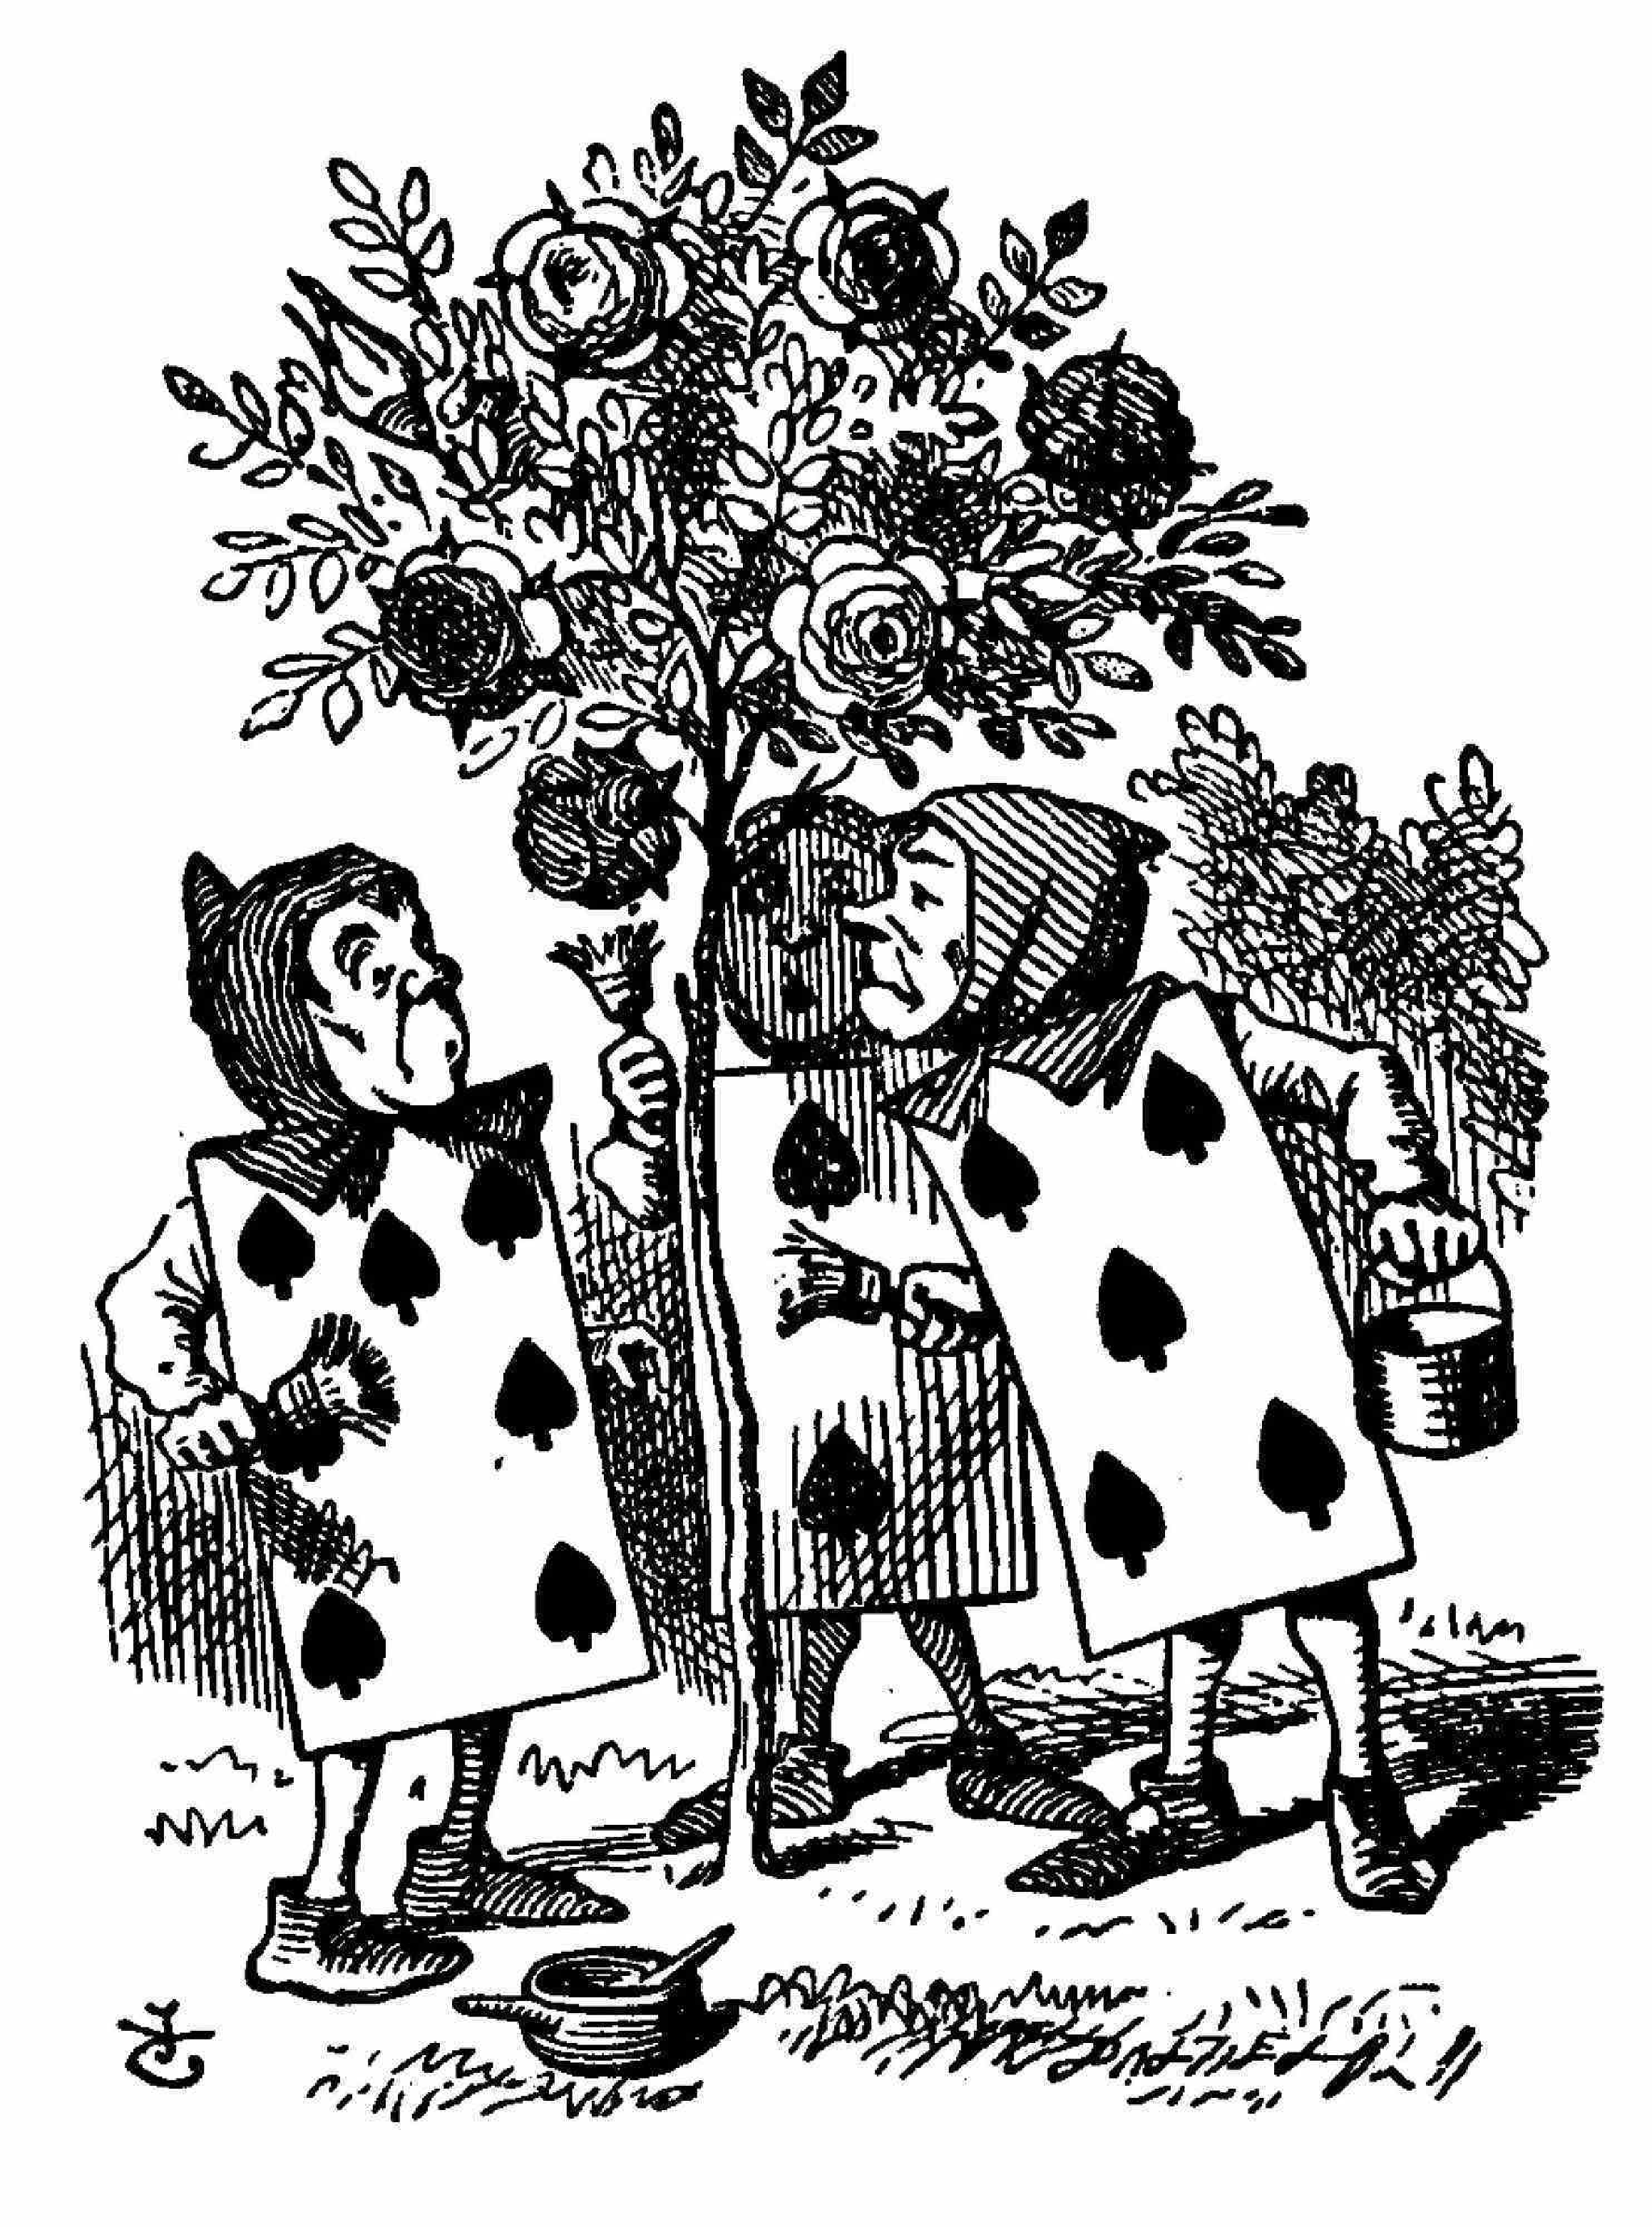
\includepdf[scale=.7]{alice_9.pdf}
% \includepdf[scale=.8]{escher_spiral_fish_gray.pdf}
% \chapter*{\hypertarget{chwiener}{\hspace{1cm}\normalfont\textbf{Appendice}}}
\chapter*{\hypertarget{chwiener}{\hspace{.55cm}\normalfont\textbf{Appendice}}}
\chaptermark{Appendice}
\addcontentsline{toc}{chapter}{Appendice}
% \begin{fullwidth}
%   \begin{changemargin}{1cm}{1cm}
%     \setlength{\parindent}{1.5ex}
%     \lipsum[1-2]

%     \lipsum[1]
%   \end{changemargin}
% \end{fullwidth}
% \includepdf[scale=1]{attacco_classico.pdf}
% \includepdf[scale=1]{attacco_esteso.pdf}
\begin{tcolorbox}[enhanced, breakable, colback=white, colframe=white, check odd page, toggle left and right, grow to right by=\marginparwidth+\marginparsep, toggle enlargement=evenpage]
  \setlength{\parindent}{2ex}
  % \lipsum[1-4]
  % \lstinputlisting{final_test.wl}
  \section*{\normalfont\textbf{Implementazione Attacco Classico in \textit{Mathematica\textsuperscript{\textregistered}}}}
  \begin{lstlisting}
    e = 7502876735617; n = 28562942440499; (*esempio di chiave pubblica attaccabile*)
    fc = ContinuedFraction[e/n];
    cList = Convergents[fc];
    phiList = Floor[e/Rest[cList]];\end{lstlisting}
  \begin{lstlisting}
    check[phi_] := (x/.p) /; (Mod[n,x] /. (p=Solve[x^2-(n-phi+1)x+n==0,x])) == {0, 0};
    checkL[phi_List] := Flatten[Cases[check /@ phi,_List]];\end{lstlisting}
  \begin{lstlisting}
    primes = Flatten[checkL /@ (phiList-m /. {m->#}& /@ Range[0,9])];\end{lstlisting}
\end{tcolorbox}
\vspace{1.5cm}
\begin{tcolorbox}[enhanced, breakable, colback=white, colframe=white, check odd page, toggle left and right, grow to right by=\marginparwidth+\marginparsep, toggle enlargement=evenpage]
  \setlength{\parindent}{2ex}
  \section*{\normalfont\textbf{Implementazione Attacco Esteso in \textit{Mathematica\textsuperscript{\textregistered}}}}
  \begin{lstlisting}
    r = 4; Dl = 2; (*da regolare in base alle esigenze del caso*)
    CClist = Partition[Rest[cList],2,1];
    UVlist = Tuples[Range[2^r],2];
    T = Tuples[{CClist,UVlist}];
    phiList = Floor[
      e(T[[2,1]]Denominator[T[[1,2]]]+(T[[2,1]]Dl+T[[2,2]])Denominator[T[[1,1]]])/
       (T[[2,1]] Numerator[T[[1,2]]]+(T[[2,1]]Dl+T[[2,2]])Numerator[T[[1,1]]])];\end{lstlisting}
  \begin{lstlisting}
    primes = Flatten[checkL /@ (phiList-m /. {m->#}& /@ Range[0,9])];\end{lstlisting}
  % \begin{lstlisting}
  %   CF[n_]:=
	%     Module[{A=Append[{},Floor[n]],x=1/FractionalPart[n]},
	% 	    While[FractionalPart[x]!=0,
	% 		    AppendTo[A,Floor[x]];
	% 		    x=1/FractionalPart[x];
	% 	    ];
	% 	    AppendTo[A,Floor[x]];A
  %       ]

  %   ConvF[eList_]:=
	%     Module[{cList=Append[{},eList[[1]]],a=-1,a1=eList[[1]],a2=1,b=-1,b1=1,b2=0},
	% 	    Do[
	% 		    a=eList[[i]]*a1+a2;
	% 		    b=eList[[i]]*b1+b2;
	% 		    AppendTo[cList,a/b];
	% 		    a2=a1;a1=a;b2=b1;b1=b,
	% 	    {i,2,Length[eList]}];
	% 	    cList
  %       ]\end{lstlisting}
  % \begin{lstlisting}
  %   Verifica[N_,phi_]:=
	%     Module[{x,p},
	% 	    If[(Mod[N,x]/.(p=Solve[x^2-(N-phi+1)*x+N==0,x]))=={0,0},x/.p,False]
  %       ]
    
  %   Couples[s_List]:=Couples[s]=
  %       If[Length[s]<2,{},(Prepend[Couples[Rest[s]],{First[#],First[Rest[#]]}])&[s]]\end{lstlisting}\newpage

  % \begin{lstlisting}
  %   Wiener[e_,N_]:=
  %       Module[{phiList=Floor[e/Rest[ConvF[CF[e/N]]]],primes=False,m=0,i},
  %           While[!primes && m<10,i=0;
  %               While[++i<=Length[phiList] && !(primes=Verifica[N,phiList[[i]]]),];
  %               phiList=(++m)+phiList;
  %           ];
  %           primes
  %       ]

  %   ExtWiener[e_,N_,r_,Dl_]:=
  %       Module[{A=Numerator[Couples[Rest[ConvF[CF[e/N]]]]],
  %               B=Denominator[Couples[Rest[ConvF[CF[e/N]]]]],
  %               UV=Tuples[Range[2^r],2],
  %               BruteF,phi,k,m=-1,i=0,primes=False},
  %           BruteF[x_List]:=For[k=1,k<=Length[x] && !primes,k++,
  %                   phi=Floor[e/((x[[k,1]]*A[[i,2]]+(x[[k,1]]*Dl+x[[k,2]])*A[[i,1]])/
  %                           (x[[k,1]]*B[[i,2]]+(x[[k,1]]*Dl+x[[k,2]])*B[[i,1]]))]+m;
  %                   primes=Verifica[N,phi];
  %           ];
  %           While[++m<10 && !primes,i=0;
  %               While[++i<=Length[A] && !primes, BruteF[UV]];
  %           ];
  %           primes
  %       ]\end{lstlisting}
\end{tcolorbox}




% % \chapter[On the Use of the tufte-book Document Class]{On the Use of the \texttt{tufte-book} Document Class}
% \label{ch:tufte-book}

% The \TL document classes define a style similar to the
% style Edward Tufte uses in his books and handouts.  Tufte's style is known
% for its extensive use of sidenotes, tight integration of graphics with
% text, and well-set typography.  This document aims to be at once a
% demonstration of the features of the \TL document classes
% and a style guide to their use.

% \section*{Page Layout}\label{sec:page-layout}
% \subsection*{Headings}\label{sec:headings}\index{headings}
% This style provides \textsc{a}- and \textsc{b}-heads (that is,
% \Verb|\section| and \Verb|\subsection|), demonstrated above.

% If you need more than two levels of section headings, you'll have to define
% them yourself at the moment; there are no pre-defined styles for anything below
% a \Verb|\subsection|.  As Bringhurst points out in \textit{The Elements of
% Typographic Style},\cite{Bringhurst2005} you should ``use as many levels of
% headings as you need: no more, and no fewer.''

% The \TL classes will emit an error if you try to use
% \linebreak\Verb|\subsubsection| and smaller headings.

% % let's start a new thought -- a new section
% \newthought{In his later books},\cite{Tufte2006} Tufte
% starts each section with a bit of vertical space, a non-indented paragraph,
% and sets the first few words of the sentence in \textsc{small caps}.  To
% accomplish this using this style, use the \doccmddef{newthought} command:
% \begin{docspec}
%   \doccmd{newthought}\{In his later books\}, Tufte starts\ldots
% \end{docspec}


% \section*{Sidenotes}\label{sec:sidenotes}
% One of the most prominent and distinctive features of this style is the
% extensive use of sidenotes.  There is a wide margin to provide ample room
% for sidenotes and small figures.  Any \doccmd{footnote}s will automatically
% be converted to sidenotes.\footnote{This is a sidenote that was entered
% using the \texttt{\textbackslash footnote} command.}  If you'd like to place ancillary
% information in the margin without the sidenote mark (the superscript
% number), you can use the \doccmd{marginnote} command.\marginnote{\textit{This is a
% margin note.  Notice that there isn't a number preceding the note, and
% there is no number in the main text where this note was written.
% \lipsum[2-3]}}

% The specification of the \doccmddef{sidenote} command is:
% \begin{docspec}
%   \doccmd{sidenote}[\docopt{number}][\docopt{offset}]\{\docarg{Sidenote text.}\}
% \end{docspec}

% Both the \docopt{number} and \docopt{offset} arguments are optional.  If you
% provide a \docopt{number} argument, then that number will be used as the
% sidenote number.  It will change of the number of the current sidenote only and
% will not affect the numbering sequence of subsequent sidenotes.

% Sometimes a sidenote may run over the top of other text or graphics in the
% margin space.  If this happens, you can adjust the vertical position of the
% sidenote by providing a dimension in the \docopt{offset} argument.  Some
% examples of valid dimensions are:
% \begin{docspec}
%   \ttfamily 1.0in \qquad 2.54cm \qquad 254mm \qquad 6\Verb|\baselineskip|
% \end{docspec}
% If the dimension is positive it will push the sidenote down the page; if the
% dimension is negative, it will move the sidenote up the page.

% While both the \docopt{number} and \docopt{offset} arguments are optional, they
% must be provided in order.  To adjust the vertical position of the sidenote
% while leaving the sidenote number alone, use the following syntax:
% \begin{docspec}
%   \doccmd{sidenote}[][\docopt{offset}]\{\docarg{Sidenote text.}\}
% \end{docspec}
% The empty brackets tell the \Verb|\sidenote| command to use the default
% sidenote number.

% If you \emph{only} want to change the sidenote number, however, you may
% completely omit the \docopt{offset} argument:
% \begin{docspec}
%   \doccmd{sidenote}[\docopt{number}]\{\docarg{Sidenote text.}\}
% \end{docspec}

% The \doccmddef{marginnote} command has a similar \docarg{offset} argument:
% \begin{docspec}
%   \doccmd{marginnote}[\docopt{offset}]\{\docarg{Margin note text.}\}
% \end{docspec}

% \section*{References}
% References are placed alongside their citations as sidenotes,
% as well.  This can be accomplished using the normal \doccmddef{cite}
% command.\sidenote{The first paragraph of this document includes a citation.}

% The complete list of references may also be printed automatically by using
% the \doccmddef{bibliography} command.  (See the end of this document for an
% example.)  If you do not want to print a bibliography at the end of your
% document, use the \doccmddef{nobibliography} command in its place.  

% % To enter multiple citations at one location,\cite[-3\baselineskip]{Tufte2006,Tufte1990} you can
% provide a list of keys separated by commas and the same optional vertical
% offset argument: \Verb|\cite{Tufte2006,Tufte1990}|.  
% \begin{docspec}
%   \doccmd{cite}[\docopt{offset}]\{\docarg{bibkey1,bibkey2,\ldots}\}
% \end{docspec}

% \section*{Figures and Tables}\label{sec:figures-and-tables}
% Images and graphics play an integral role in Tufte's work.
% In addition to the standard \docenvdef{figure} and \docenvdef{tabular} environments,
% this style provides special figure and table environments for full-width
% floats.

% Full page--width figures and tables may be placed in \docenvdef{figure*} or
% \docenvdef{table*} environments.  To place figures or tables in the margin,
% use the \docenvdef{marginfigure} or \docenvdef{margintable} environments as follows
% (see figure~\ref{fig:marginfig}):

% \begin{marginfigure}%
%   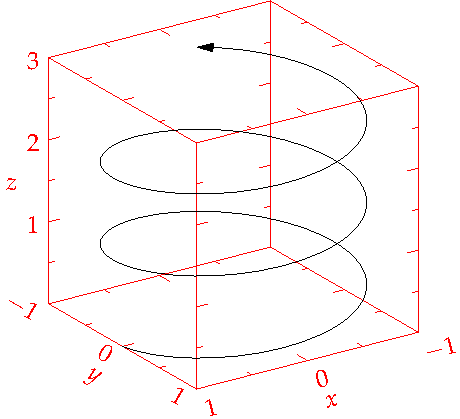
\includegraphics[width=\linewidth]{helix}
%   \caption{This is a margin figure.  The helix is defined by 
%     $x = \cos(2\pi z)$, $y = \sin(2\pi z)$, and $z = [0, 2.7]$.  The figure was
%     drawn using Asymptote (\url{http://asymptote.sf.net/}).}
%   \label{fig:marginfig}
% \end{marginfigure}

% \begin{docspec}
% \textbackslash begin\{marginfigure\}\\
%   \qquad\textbackslash includegraphics\{helix\}\\
%   \qquad\textbackslash caption\{This is a margin figure.\}\\
%   \qquad\textbackslash label\{fig:marginfig\}\\
% \textbackslash end\{marginfigure\}\\
% \end{docspec}

% The \docenv{marginfigure} and \docenv{margintable} environments accept an optional parameter \docopt{offset} that adjusts the vertical position of the figure or table.  See the ``\nameref{sec:sidenotes}'' section above for examples.  The specifications are:
% \begin{docspec}
%   \textbackslash{begin\{marginfigure\}[\docopt{offset}]}\\
%   \qquad\ldots\\
%   \textbackslash{end\{marginfigure\}}\\
%   \mbox{}\\
%   \textbackslash{begin\{margintable\}[\docopt{offset}]}\\
%   \qquad\ldots\\
%   \textbackslash{end\{margintable\}}\\
% \end{docspec}

% Figure~\ref{fig:fullfig} is an example of the \docenv{figure*}
% environment and figure~\ref{fig:textfig} is an example of the normal
% \docenv{figure} environment.

% \begin{figure*}[h]
%   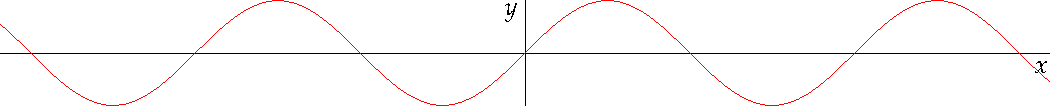
\includegraphics[width=\linewidth]{sine.pdf}%
%   \caption{This graph shows $y = \sin x$ from about $x = [-10, 10]$.
%   \emph{Notice that this figure takes up the full page width.}}%
%   \label{fig:fullfig}%
% \end{figure*}

% \begin{figure}
%   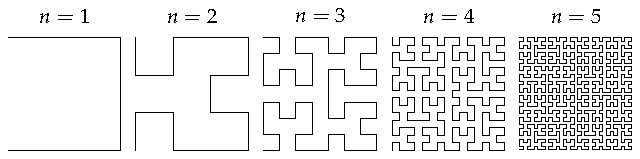
\includegraphics{hilbertcurves.pdf}
% %  \checkparity This is an \pageparity\ page.%
%   \caption[Hilbert curves of various degrees $n$.][6pt]{Hilbert curves of various degrees $n$. \emph{Notice that this figure only takes up the main textblock width.}}
%   \label{fig:textfig}
%   %\zsavepos{pos:textfig}
% \end{figure}

% As with sidenotes and marginnotes, a caption may sometimes require vertical
% adjustment. The \doccmddef{caption} command now takes a second optional
% argument that enables you to do this by providing a dimension \docopt{offset}.
% You may specify the caption in any one of the following forms:
% \begin{docspec}
%   \doccmd{caption}\{\docarg{long caption}\}\\
%   \doccmd{caption}[\docarg{short caption}]\{\docarg{long caption}\}\\
%   \doccmd{caption}[][\docopt{offset}]\{\docarg{long caption}\}\\
%   \doccmd{caption}[\docarg{short caption}][\docopt{offset}]%
%                   \{\docarg{long caption}\}
% \end{docspec}
% A positive \docopt{offset} will push the caption down the page. The short
% caption, if provided, is what appears in the list of figures/tables, otherwise
% the ``long'' caption appears there. Note that although the arguments
% \docopt{short caption} and \docopt{offset} are both optional, they must be
% provided in order. Thus, to specify an \docopt{offset} without specifying a
% \docopt{short caption}, you must include the first set of empty brackets
% \Verb|[]|, which tell \doccmd{caption} to use the default ``long'' caption. As
% an example, the caption to figure~\ref{fig:textfig} above was given in the form
% \begin{docspec}
%   \doccmd{caption}[Hilbert curves...][6pt]\{Hilbert curves...\}
% \end{docspec}

% Table~\ref{tab:normaltab} shows table created with the \docpkg{booktabs}
% package.  Notice the lack of vertical rules---they serve only to clutter
% the table's data.

% \begin{table}[ht]
%   \centering
%   \fontfamily{ppl}\selectfont
%   \begin{tabular}{ll}
%     \toprule
%     Margin & Length \\
%     \midrule
%     Paper width & \unit[8\nicefrac{1}{2}]{inches} \\
%     Paper height & \unit[11]{inches} \\
%     Textblock width & \unit[6\nicefrac{1}{2}]{inches} \\
%     Textblock/sidenote gutter & \unit[\nicefrac{3}{8}]{inches} \\
%     Sidenote width & \unit[2]{inches} \\
%     \bottomrule
%   \end{tabular}
%   \caption{Here are the dimensions of the various margins used in the Tufte-handout class.}
%   \label{tab:normaltab}
%   %\zsavepos{pos:normaltab}
% \end{table}

% \newthought{Occasionally} \LaTeX{} will generate an error message:\label{err:too-many-floats}
% \begin{docspec}
%   Error: Too many unprocessed floats
% \end{docspec}
% \LaTeX{} tries to place floats in the best position on the page.  Until it's
% finished composing the page, however, it won't know where those positions are.
% If you have a lot of floats on a page (including sidenotes, margin notes,
% figures, tables, etc.), \LaTeX{} may run out of ``slots'' to keep track of them
% and will generate the above error.

% \LaTeX{} initially allocates 18 slots for storing floats.  To work around this
% limitation, the \TL document classes provide a \doccmddef{morefloats} command
% that will reserve more slots.

% The first time \doccmd{morefloats} is called, it allocates an additional 34
% slots.  The second time \doccmd{morefloats} is called, it allocates another 26
% slots.

% The \doccmd{morefloats} command may only be used two times.  Calling it a
% third time will generate an error message.  (This is because we can't safely
% allocate many more floats or \LaTeX{} will run out of memory.)

% If, after using the \doccmd{morefloats} command twice, you continue to get the
% \texttt{Too many unprocessed floats} error, there are a couple things you can
% do.

% The \doccmddef{FloatBarrier} command will immediately process all the floats
% before typesetting more material.  Since \doccmd{FloatBarrier} will start a new
% paragraph, you should place this command at the beginning or end of a
% paragraph.

% The \doccmddef{clearpage} command will also process the floats before
% continuing, but instead of starting a new paragraph, it will start a new page.

% You can also try moving your floats around a bit: move a figure or table to the
% next page or reduce the number of sidenotes.  (Each sidenote actually uses
% \emph{two} slots.)

% After the floats have placed, \LaTeX{} will mark those slots as unused so they
% are available for the next page to be composed.

% \section*{Captions}
% You may notice that the captions are sometimes misaligned.
% Due to the way \LaTeX's float mechanism works, we can't know for sure where it
% decided to put a float. Therefore, the \TL document classes provide commands to
% override the caption position.

% \paragraph{Vertical alignment} To override the vertical alignment, use the
% \doccmd{setfloatalignment} command inside the float environment.  For
% example:

% \begin{fullwidth}
% \begin{docspec}
%   \textbackslash begin\{figure\}[btp]\\
%   \qquad \textbackslash includegraphics\{sinewave\}\\
%   \qquad \textbackslash caption\{This is an example of a sine wave.\}\\
%   \qquad \textbackslash label\{fig:sinewave\}\\
%   \qquad \hlred{\textbackslash setfloatalignment\{b\}\% forces caption to be bottom-aligned}\\
%   \textbackslash end\{figure\}
% \end{docspec}
% \end{fullwidth}

% \noindent The syntax of the \doccmddef{setfloatalignment} command is:

% \begin{docspec}
%   \doccmd{setfloatalignment}\{\docopt{pos}\}
% \end{docspec}

% \noindent where \docopt{pos} can be either \texttt{b} for bottom-aligned
% captions, or \texttt{t} for top-aligned captions.

% \paragraph{Horizontal alignment}\label{par:overriding-horizontal}
% To override the horizontal alignment, use either the \doccmd{forceversofloat}
% or the \doccmd{forcerectofloat} command inside of the float environment.  For
% example:

% \begin{fullwidth}
% \begin{docspec}
%   \textbackslash begin\{figure\}[btp]\\
%   \qquad \textbackslash includegraphics\{sinewave\}\\
%   \qquad \textbackslash caption\{This is an example of a sine wave.\}\\
%   \qquad \textbackslash label\{fig:sinewave\}\\
%   \qquad \hlred{\textbackslash forceversofloat\% forces caption to be set to the left of the float}\\
%   \textbackslash end\{figure\}
% \end{docspec}
% \end{fullwidth}

% The \doccmddef{forceversofloat} command causes the algorithm to assume the
% float has been placed on a verso page---that is, a page on the left side of a
% two-page spread.  Conversely, the \doccmddef{forcerectofloat} command causes
% the algorithm to assume the float has been placed on a recto page---that is, a
% page on the right side of a two-page spread.


% \section*{Full-width text blocks}

% In addition to the new float types, there is a \docenvdef{fullwidth}
% environment that stretches across the main text block and the sidenotes
% area.

% \begin{Verbatim}
% \begin{fullwidth}
% Lorem ipsum dolor sit amet...
% \end{fullwidth}
% \end{Verbatim}

% \begin{fullwidth}
% \small\itshape\lipsum[1]
% \end{fullwidth}

% \section*{Typography}\label{sec:typography}

% \subsection*{Typefaces}\label{sec:typefaces}\index{typefaces}
% If the Palatino, \textsf{Helvetica}, and \texttt{Bera Mono} typefaces are installed, this style
% will use them automatically.  Otherwise, we'll fall back on the Computer Modern
% typefaces.

% \subsection*{Letterspacing}\label{sec:letterspacing}
% This document class includes two new commands and some improvements on
% existing commands for letterspacing.

% When setting strings of \allcaps{ALL CAPS} or \smallcaps{small caps}, the
% letter\-spacing---that is, the spacing between the letters---should be
% increased slightly.\cite{Bringhurst2005}  The \doccmddef{allcaps} command has proper letterspacing for
% strings of \allcaps{FULL CAPITAL LETTERS}, and the \doccmddef{smallcaps} command
% has letterspacing for \smallcaps{small capital letters}.  These commands
% will also automatically convert the case of the text to upper- or
% lowercase, respectively.

% The \doccmddef{textsc} command has also been redefined to include
% letterspacing.  The case of the \doccmd{textsc} argument is left as is,
% however.  This allows one to use both uppercase and lowercase letters:
% \textsc{The Initial Letters Of The Words In This Sentence Are Capitalized.}



% \section*{Document Class Options}\label{sec:options}

% \index{class options|(}
% The \doccls{tufte-book} class is based on the \LaTeX\ \doccls{book}
% document class.  Therefore, you can pass any of the typical book
% options.  There are a few options that are specific to the
% \doccls{tufte-book} document class, however.

% The \docclsoptdef{a4paper} option will set the paper size to \smallcaps{A4} instead of
% the default \smallcaps{US} letter size.

% The \docclsoptdef{sfsidenotes} option will set the sidenotes and title block in a 
% \textsf{sans serif} typeface instead of the default roman.

% The \docclsoptdef{twoside} option will modify the running heads so that the page
% number is printed on the outside edge (as opposed to always printing the page
% number on the right-side edge in \docclsoptdef{oneside} mode).  

% The \docclsoptdef{symmetric} option typesets the sidenotes on the outside edge of
% the page.  This is how books are traditionally printed, but is contrary to
% Tufte's book design which sets the sidenotes on the right side of the page.
% This option implicitly sets the \docclsopt{twoside} option.

% The \docclsoptdef{justified} option sets all the text fully justified (flush left
% and right).  The default is to set the text ragged right.  
% The body text of Tufte's books are set ragged right.  This prevents
% needless hyphenation and makes it easier to read the text in the slightly
% narrower column.

% The \docclsoptdef{bidi} option loads the \docpkg{bidi} package which is used with
% \tXeLaTeX\ to typeset bi-directional text.  Since the \docpkg{bidi}
% package needs to be loaded before the sidenotes and cite commands are defined,
% it can't be loaded in the document preamble.

% The \docclsoptdef{debug} option causes the \TL classes to output debug
% information to the log file which is useful in troubleshooting bugs.  It will
% also cause the graphics to be replaced by outlines.

% The \docclsoptdef{nofonts} option prevents the \TL classes from
% automatically loading the Palatino and Helvetica typefaces.  You should use
% this option if you wish to load your own fonts.  If you're using \tXeLaTeX, this
% option is implied (\ie, the Palatino and Helvetica fonts aren't loaded if you
% use \tXeLaTeX).  

% The \docclsoptdef{nols} option inhibits the letterspacing code.  The \TL\
% classes try to load the appropriate letterspacing package (either pdf\TeX's
% \docpkg{letterspace} package or the \docpkg{soul} package).  If you're using
% \tXeLaTeX\ with \docpkg{fontenc}, however, you should configure your own
% letterspacing.  

% The \docclsoptdef{notitlepage} option causes \doccmd{maketitle} to generate a title
% block instead of a title page.  The \doccls{book} class defaults to a title
% page and the \doccls{handout} class defaults to the title block.  There is an
% analogous \docclsoptdef{titlepage} option that forces \doccmd{maketitle} to
% generate a full title page instead of the title block.

% The \docclsoptdef{notoc} option suppresses \TL's custom table of contents
% (\textsc{toc}) design.  The current \textsc{toc} design only shows unnumbered
% chapter titles; it doesn't show sections or subsections.  The \docclsopt{notoc}
% option will revert to \LaTeX's \textsc{toc} design.

% The \docclsoptdef{nohyper} option prevents the \docpkg{hyperref} package from
% being loaded.  The default is to load the \docpkg{hyperref} package and use the
% \doccmd{title} and \doccmd{author} contents as metadata for the generated
% \textsc{pdf}.

% \index{class options|)}



% \chapter*[Customizing Tufte-LaTeX]{Customizing \TL}
% \label{ch:customizing}

% The \TL document classes are designed to closely emulate Tufte's book
% design by default.  However, each document is different and you may encounter
% situations where the default settings are insufficient.  This chapter explores
% many of the ways you can adjust the \TL document classes to better fit
% your needs.

% \section*{File Hooks}
% \label{sec:filehooks}

% \index{file hooks|(}
% If you create many documents using the \TL classes, it's easier to
% store your customizations in a separate file instead of copying them into the
% preamble of each document.  The \TL classes provide three file hooks:
% \docfilehook{tufte-common-local.tex}{common}, \docfilehook{tufte-book-local.tex}{book}, and
% \docfilehook{tufte-handout-local.tex}{handout}.\sloppy

% \begin{description}
%   \item[\docfilehook{tufte-common-local.tex}{common}]
%     If this file exists, it will be loaded by all of the \TL document
%     classes just prior to any document-class-specific code.  If your
%     customizations or code should be included in both the book and handout
%     classes, use this file hook.
%   \item[\docfilehook{tufte-book-local.tex}{book}] 
%     If this file exists, it will be loaded after all of the common and
%     book-specific code has been read.  If your customizations apply only to the
%     book class, use this file hook.
%   \item[\docfilehook{tufte-common-handout.tex}{handout}] 
%     If this file exists, it will be loaded after all of the common and
%     handout-specific code has been read.  If your customizations apply only to
%     the handout class, use this file hook.
% \end{description}

% \index{file hooks|)}

% \section*{Numbered Section Headings}
% \label{sec:numbered-sections}
% \index{headings!numbered}

% While Tufte dispenses with numbered headings in his books, if you require them,
% they can be anabled by changing the value of the \doccounter{secnumdepth}
% counter.  From the table below, select the heading level at which numbering
% should stop and set the \doccounter{secnumdepth} counter to that value.  For
% example, if you want parts and chapters numbered, but don't want numbering for
% sections or subsections, use the command:
% \begin{docspec}
%   \doccmd{setcounter}\{secnumdepth\}\{0\}
% \end{docspec}

% The default \doccounter{secnumdepth} for the \TL document classes is $-1$.

% \begin{table}
%   \footnotesize
%   \begin{center}
%     \begin{tabular}{lr}
%       \toprule
%       Heading level & Value \\
%       \midrule
%       Part (in \doccls{tufte-book}) & $-1$ \\
%       Part (in \doccls{tufte-handout}) & $0$ \\
%       Chapter (only in \doccls{tufte-book}) & $0$ \\
%       Section & $1$ \\
%       Subsection & $2$ \\
%       Subsubsection & $3$ \\
%       Paragraph & $4$ \\
%       Subparagraph & $5$ \\
%       \bottomrule
%     \end{tabular}
%   \end{center}
%   \caption{Heading levels used with the \texttt{secnumdepth} counter.}
% \end{table}

% \section*{Changing the Paper Size}
% \label{sec:paper-size}

% The \TL classes currently only provide three paper sizes: \textsc{a4},
% \textsc{b5}, and \textsc{us} letter.  To specify a different paper size (and/or
% margins), use the \doccmd[geometry]{geometry} command in the preamble of your
% document (or one of the file hooks).  The full documentation of the
% \doccmd{geometry} command may be found in the \docpkg{geometry} package
% documentation.\cite{pkg-geometry}


% \section*{Customizing Marginal Material}
% \label{sec:marginal-material}

% Marginal material includes sidenotes, citations, margin notes, and captions.
% Normally, the justification of the marginal material follows the justification
% of the body text.  If you specify the \docclsopt{justified} document class
% option, all of the margin material will be fully justified as well.  If you
% don't specify the \docclsopt{justified} option, then the marginal material will
% be set ragged right.

% You can set the justification of the marginal material separately from the body
% text using the following document class options: \docclsopt{sidenote},
% \docclsopt{marginnote}, \docclsopt{caption}, \docclsopt{citation}, and
% \docclsopt{marginals}.  Each option refers to its obviously corresponding
% marginal material type.  The \docclsopt{marginals} option simultaneously sets
% the justification on all four marginal material types.

% Each of the document class options takes one of five justification types:
% \begin{description}
%   \item[\docclsopt{justified}] Fully justifies the text (sets it flush left and
%     right).
%   \item[\docclsopt{raggedleft}] Sets the text ragged left, regardless of which
%     page it falls on.
%   \item[\docclsopt{raggedright}] Sets the text ragged right, regardless of
%     which page it falls on.
%   \item[\doccls{raggedouter}] Sets the text ragged left if it falls on the
%     left-hand (verso) page of the spread and otherwise sets it ragged right.
%     This is useful in conjunction with the \docclsopt{symmetric} document class
%     option.
%   \item[\docclsopt{auto}] If the \docclsopt{justified} document class option
%     was specified, then set the text fully justified; otherwise the text is set
%     ragged right.  This is the default justification option if one is not
%     explicitly specified.
% \end{description}

% \noindent For example, 
% \begin{docspec}
%   \doccmdnoindex{documentclass}[symmetric,justified,marginals=raggedouter]\{tufte-book\}
% \end{docspec}
% will set the body text of the document to be fully justified and all of the
% margin material (sidenotes, margin notes, captions, and citations) to be flush
% against the body text with ragged outer edges.

% \newthought{The font and style} of the marginal material may also be modified using the following commands:

% \begin{docspec}
%   \doccmd{setsidenotefont}\{\docopt{font commands}\}\\
%   \doccmd{setcaptionfont}\{\docopt{font commands}\}\\
%   \doccmd{setmarginnotefont}\{\docopt{font commands}\}\\
%   \doccmd{setcitationfont}\{\docopt{font commands}\}
% \end{docspec}

% The \doccmddef{setsidenotefont} sets the font and style for sidenotes, the
% \doccmddef{setcaptionfont} for captions, the \doccmddef{setmarginnotefont} for
% margin notes, and the \doccmddef{setcitationfont} for citations.  The
% \docopt{font commands} can contain font size changes (e.g.,
% \doccmdnoindex{footnotesize}, \doccmdnoindex{Huge}, etc.), font style changes (e.g.,
% \doccmdnoindex{sffamily}, \doccmdnoindex{ttfamily}, \doccmdnoindex{itshape}, etc.), color changes (e.g.,
% \doccmdnoindex{color}\texttt{\{blue\}}), and many other adjustments.

% If, for example, you wanted the captions to be set in italic sans serif, you could use:
% \begin{docspec}
%   \doccmd{setcaptionfont}\{\doccmdnoindex{itshape}\doccmdnoindex{sffamily}\}
% \end{docspec}

% \chapter*{Compatibility Issues}
% \label{ch:compatibility}

% When switching an existing document from one document class to a \TL document class, a few changes to the document may have to be made.

% \section*{Converting from \doccls{article} to \doccls{tufte-handout}}

% The following \doccls{article} class options are unsupported: \docclsopt{10pt}, \docclsopt{11pt}, \docclsopt{12pt}, \docclsopt{a5paper}, \docclsopt{b5paper}, \docclsopt{executivepaper}, \docclsopt{legalpaper}, \docclsopt{landscape}, \docclsopt{onecolumn}, and \doccls{twocolumn}.

% The following headings are not supported: \doccmd{subsubsection} and \doccmd{subparagraph}.

% \section*{Converting from \doccls{book} to \doccls{tufte-book}}

% The following \doccls{report} class options are unsupported: \docclsopt{10pt}, \docclsopt{11pt}, \docclsopt{12pt}, \docclsopt{a5paper}, \docclsopt{b5paper}, \docclsopt{executivepaper}, \docclsopt{legalpaper}, \docclsopt{landscape}, \docclsopt{onecolumn}, and \doccls{twocolumn}.

% The following headings are not supported: \doccmd{subsubsection} and \doccmd{subparagraph}.



% \chapter*{Troubleshooting and Support}
% \label{ch:troubleshooting}

% \section*{\TL Website}\label{sec:website}
% The website for the \TL packages is located at
% \url{http://code.google.com/p/tufte-latex/}.  On our website, you'll find
% links to our \smallcaps{svn} repository, mailing lists, bug tracker, and documentation.

% \section*{\TL Mailing Lists}\label{sec:mailing-lists}
% There are two mailing lists for the \TL project:

% \paragraph{Discussion list}
% The \texttt{tufte-latex} discussion list is for asking questions, getting
% assistance with problems, and help with troubleshooting.  Release announcements
% are also posted to this list.  You can subscribe to the \texttt{tufte-latex}
% discussion list at \url{http://groups.google.com/group/tufte-latex}.

% \paragraph{Commits list}
% The \texttt{tufte-latex-commits} list is a read-only mailing list.  A message
% is sent to the list any time the \TL code has been updated.  If you'd like to
% keep up with the latest code developments, you may subscribe to this list.  You
% can subscribe to the \texttt{tufte-latex-commits} mailing list at
% \url{http://groups.google.com/group/tufte-latex-commits}.

% \section*{Getting Help}\label{sec:getting-help}
% If you've encountered a problem with one of the \TL document classes, have a
% question, or would like to report a bug, please send an email to our
% mailing list or visit our website.

% To help us troubleshoot the problem more quickly, please try to compile your
% document using the \docclsopt{debug} class option and send the generated
% \texttt{.log} file to the mailing list with a brief description of the problem.



% \section*{Errors, Warnings, and Informational Messages}\label{sec:tl-messages}
% The following is a list of all of the errors, warnings, and other messages generated by the \TL classes and a brief description of their meanings.
% \index{error messages}\index{warning messages}\index{debug messages}

% % Errors
% \docmsg{Error: \doccmd{subparagraph} is undefined by this class.}{%
% The \doccmd{subparagraph} command is not defined in the \TL document classes.
% If you'd like to use the \doccmd{subparagraph} command, you'll need to redefine
% it yourself.  See the ``Headings'' section on page~\pageref{sec:headings} for a
% description of the heading styles available in the \TL document classes.}

% \docmsg{Error: \doccmd{subsubsection} is undefined by this class.}{%
% The \doccmd{subsubsection} command is not defined in the \TL document classes.
% If you'd like to use the \doccmd{subsubsection} command, you'll need to
% redefine it yourself.  See the ``Headings'' section on
% page~\pageref{sec:headings} for a description of the heading styles available
% in the \TL document classes.}

% \docmsg{Error: You may only call \doccmd{morefloats} twice. See the\par\noindent\ \ \ \ \ \ \ \ Tufte-LaTeX documentation for other workarounds.}{%
% \LaTeX{} allocates 18 slots for storing floats.  The first time
% \doccmd{morefloats} is called, it allocates an additional 34 slots.  The second
% time \doccmd{morefloats} is called, it allocates another 26 slots.

% The \doccmd{morefloats} command may only be called two times.  Calling it a
% third time will generate this error message.  See
% page~\pageref{err:too-many-floats} for more information.}

% % Warnings
% \docmsg{Warning: Option `\docopt{class option}' is not supported -{}- ignoring option.}{%
% This warning appears when you've tried to use \docopt{class option} with a \TL
% document class, but \docopt{class option} isn't supported by the \TL document
% class.  In this situation, \docopt{class option} is ignored.}

% % Info / Debug messages
% \docmsg{Info: The `\docclsopt{symmetric}' option implies `\docclsopt{twoside}'}{%
% You specified the \docclsopt{symmetric} document class option.  This option automatically forces the \docclsopt{twoside} option as well.  See page~\pageref{clsopt:symmetric} for more information on the \docclsopt{symmetric} class option.}


% \section*{Package Dependencies}\label{sec:dependencies}
% The following is a list of packages that the \TL document
% classes rely upon.  Packages marked with an asterisk are optional.
% \begin{multicols}{2}
% \begin{itemize}
%   \item xifthen
%   \item ifpdf*
%   \item ifxetex*
%   \item hyperref
%   \item geometry
%   \item ragged2e
%   \item chngpage \emph{or} changepage
%   \item paralist
%   \item textcase
%   \item soul*
%   \item letterspace*
%   \item setspace
%   \item natbib \emph{and} bibentry
%   \item optparams
%   \item placeins
%   \item mathpazo*
%   \item helvet*
%   \item fontenc
%   \item beramono*
%   \item fancyhdr
%   \item xcolor
%   \item textcomp
%   \item titlesec
%   \item titletoc
% \end{itemize}
% \end{multicols}






%%
% The back matter contains appendices, bibliographies, indices, glossaries, etc.





% \clearpage\null\newpage
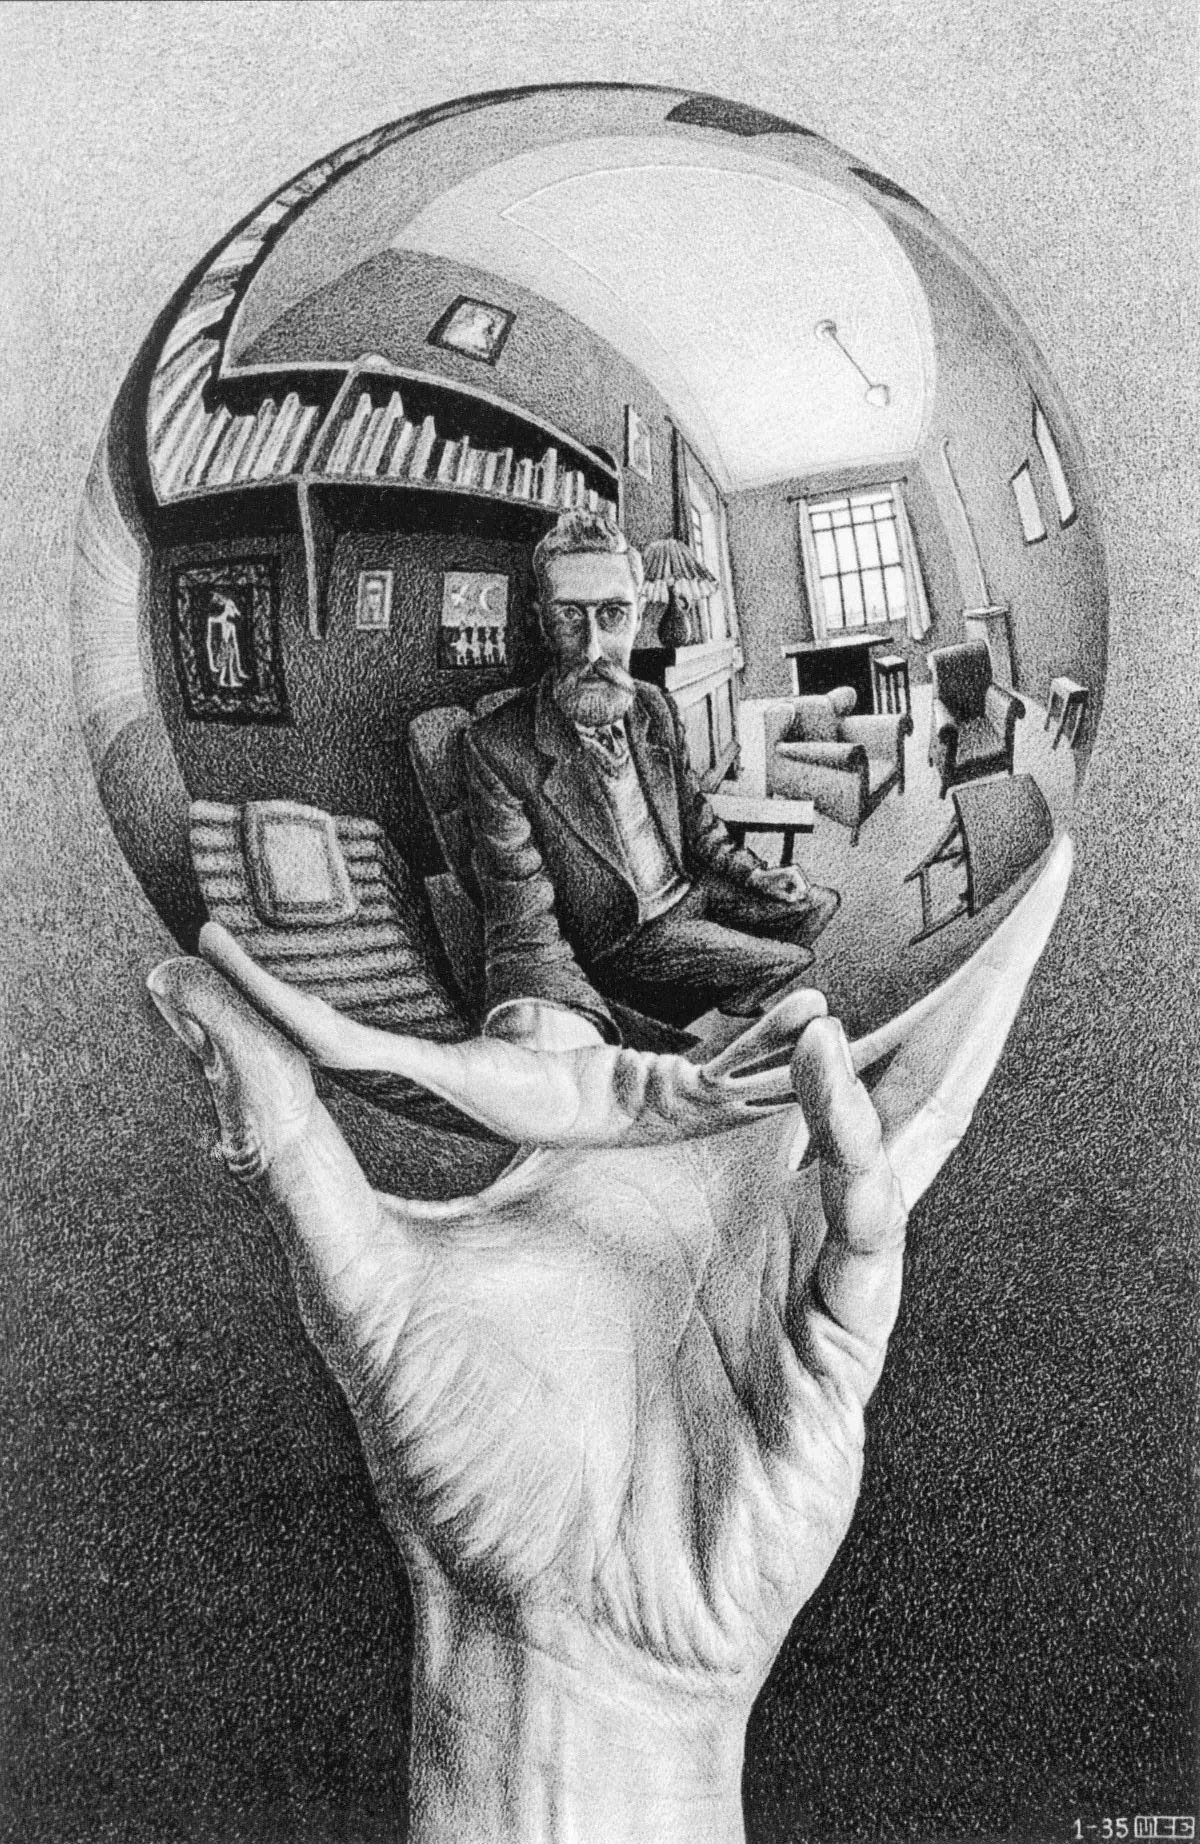
\includepdf[scale=.75]{escher_globe.pdf}
% \RaggedRight
% \backmatter

% \bibliography{sample-handout}
% \bibliographystyle{plain}

% \bibliography{\jobname}



% \printindex

\addcontentsline{toc}{chapter}{Bibliografia}
\renewcommand{\bibname}{\hspace{.05cm}\normalfont\textbf{Bibliografia}}%.55cm
\begin{thebibliography}{99}
% \begin{tcolorbox}[enhanced, breakable, colback=white, colframe=white, check odd page, toggle left and right, grow to left by=1cm, grow to right by=7.5cm, toggle enlargement=evenpage]
\begin{tcolorbox}[enhanced, breakable, colback=white, colframe=white, check odd page, toggle left and right, grow to left by=0.5cm, grow to right by=\marginparwidth+\marginparsep, toggle enlargement=evenpage]
  % \setlength{\parindent}{2ex}
  % \begin{thebibliography}{99}
    \markboth{Bibliografia}{}
    % \small
    % \begin{EmR}
    %   \raisebox{0ex}{1}
    %   \tcblower
    %   W. Diffie, M. Hellman.
    %   \href{https://www-ee.stanford.edu/~hellman/publications/24.pdf}{\textit{New Directions in Cryptography}}.
    %   \textit{IEEE Transactions on Information Theory, 1976}.
    % \end{EmR}

    \bibitem{diffie-hellman}
    W. Diffie, M. Hellman.
    % \textit{New Directions in Cryptography}.
    \href{https://www-ee.stanford.edu/~hellman/publications/24.pdf}{\textit{New Directions in Cryptography}}.
    % IEEE Trans. Inform. Theory IT-22, pag 644–654, 1976.
    \textit{IEEE Transactions on Information Theory, 1976}.
    % \url{https://www-ee.stanford.edu/~hellman/publications/24.pdf}
    

    \bibitem{rivest-shamir-edleman} 
    R.L. Rivest, A. Shamir, L. Edleman.
    \href{https://people.csail.mit.edu/rivest/Rsapaper.pdf}{\textit{A Method for Obtaining Digital Signature and Public-Key Cryptosystems}}.
    % Commun. ACM, 21(2):120–126, 1978.
    \textit{Commun. ACM, 1978}.
    

    \bibitem{superencryption} 
    G.J. Simmons, M.J. Norris.
    \href{http://www.tandfonline.com/doi/abs/10.1080/0161-117791833219}{\textit{Preliminary comments on the MIT public-key cryptosystem}}.
    % Cryptologia, 1(4):406-414, 1977.
    \textit{Cryptologia, 1977}.
    % \url{http://www.tandfonline.com/doi/abs/10.1080/0161-117791833219}
  

    \bibitem{wiener}
    M.J. Wiener.
    \href{https://sites.google.com/site/michaeljameswiener/}{\textit{Cryptanalysis of Short RSA Secret Exponents}}.
    % IEEE Transactions on Information Theory, 36(3):553–558, 1990.
    \textit{IEEE Transactions on Information Theory, 1990}.
  

    \bibitem{20y}
    D. Boneh.
    \href{https://crypto.stanford.edu/~dabo/papers/RSA-survey.pdf}{\textit{Twenty years of attacks on the RSA cryptosystem}}.
    % Notices of the American Mathematical Society, 46(2):203–213, 1999.
    \textit{Notices of the American Mathematical Society, 1999}.
  

    \bibitem{cinesi}
    M. Wu, C. Chen, Y. Lin, H. Sun.
    \href{https://www.researchgate.net/publication/263585403_On_the_Improvement_of_Wiener_Attack_on_RSA_with_Small_Private_Exponent}{\textit{On the Improvement of Wiener Attack on $RSA$ with Small Private Exponent}}.
    \textit{Scientific World Journal, 2014}.
    % \url{https://www.researchgate.net/publication/263585403_On_the_Improvement_of_Wiener_Attack_on_RSA_with_Small_Private_Exponent}
  

    \bibitem{verheul}
    E.R. Verheul, H.C.A. van Tilborg.
    \href{http://www.cs.ru.nl/~E.Verheul/papers/AiE1997/AiE1997.pdf}{\textit{Cryptanalysis of `less short' $RSA$ secret exponent}}.
    % Applicable Algebra in Engineering, Communications and Computing, vol 8, pag 425–435, 1997.
    \textit{Applicable Algebra in Engineering, Communications and Computing, 1997}.
    % \url{http://www.cs.ru.nl/~E.Verheul/papers/AiE1997/AiE1997.pdf}
  

    \bibitem{dujella}
    A. Dujella.
    \href{https://arxiv.org/pdf/cs/0402052.pdf}{\textit{Continued fractions and RSA with small secret exponent}}.
    % Tatra Mt. Math. Publ., 29:101–112, 2004.
    \textit{Tatra Mountains Mathematical Publications, 2004}.
  

    \bibitem{B-D}
    D. Boneh, G.Durfee.
    \href{http://citeseerx.ist.psu.edu/viewdoc/summary?doi=10.1.1.40.2636}{\textit{Cryptanalysis of RSA with Private Key $d$ Less Than $N^{0.292}$}}.
    \textit{Preprint, 1998}.
    % \url{http://citeseerx.ist.psu.edu/viewdoc/summary?doi=10.1.1.40.2636}
  

    \bibitem{pkcs}
    \href{https://tools.ietf.org/html/rfc8017}{\textit{PKCS $\#1$: RSA Cryptography Specifications Version 2.2}}.
    \textit{Internet Engineering Task Force, 2012}.
  

\begin{comment}
    \bibitem{knuth1} 
    D.E. Knuth.
    \textit{\color{blue} The art of computer programming, volume 1: fundamental algorithms}.
    \textit{Addison-Wesley, 3nd edition, 1997}.
  

    \bibitem{knuth2} 
    D.E. Knuth.
    \textit{\color{blue} The art of computer programming, volume 2: seminumerical algorithms}.
    \textit{Addison-Wesley, 3nd edition, 1997}.
\end{comment}


    \bibitem{hardy-apo}
    G.H. Hardy.
    \textit{A Mathematician’s Apology}.
    \textit{Cambridge University Press, 1940}.
  

    \bibitem{hardy}
    G.H. Hardy, E.M. Wright, J.H. Silverman.
    \textit{An Introduction to the Theory of Numbers}.
    \textit{Oxford University Press, 6th edition, 2008}.
  

    \bibitem{carmichael}
    R.D. Carmichael.
    \textit{The Theory of Numbers}.
    \textit{New York: John Wiley \& Sons, 1914}.
  

\begin{comment}
    \bibitem{math-crypt}
    J. Hoffstein, J. Pipher, J.H. Silverman.
    \textit{\color{blue} An Introduction to Mathematical Cryptography}.
    \textit{Springer, Undergraduate Text in Mathematics, 2th edition, 2014}.
\end{comment}
  

    \bibitem{aritmetica}
    W.M. Baldoni, C. Ciliberto, G.M. Piacentini Catteneo.
    \textit{Aritmetica, crittografia e codici}.
    \textit{Springer, 2006}.
  

    \bibitem{apostol}
    T.M. Apostol.
    \textit{Introduction to Analytic Number Theory}.
    \textit{Springer, Undergraduate Text in Mathematics, 5th edition, 1998}.
  

    \bibitem{riesel}
    H. Riesel.
    \textit{Prime Numbers and Computer Methods for Factorization}.
    \textit{Birkh\"auser, Progress in Mathematics, 1985}.
  

\begin{comment}
    \bibitem{koblitz}
    N. Koblitz.
    \textit{\color{blue} A course in number theory and cryptography}.
    \textit{Springer, Graduate Text in Mathematics, 2th edition, 1994}.
\end{comment}
  

    \bibitem{hinek}
    M.J. Hinek.
    \textit{Cryptanalysis of RSA and its variants}.
    \textit{Chapman \& Hall/CRC, Cryptography and Network Security, 2010}.
  

    \bibitem{yan}
    S.Y. Yan.
    \textit{Cryptanalytic Attacks on RSA}.
    \textit{Springer, 2008}.
  

\begin{comment}
    \bibitem{joux}
    A. Joux.
    \textit{\color{blue} Algorithmic Cryptanalysis}.
    \textit{Chapman \& Hall/CRC, 2009}.
\end{comment}


  % \end{thebibliography}
\end{tcolorbox}
\end{thebibliography}


\end{document}

